%&preformat-disser
\RequirePackage[l2tabu,orthodox]{nag} % Раскомментировав, можно в логе получать рекомендации относительно правильного использования пакетов и предупреждения об устаревших и нерекомендуемых пакетах
% Формат А4, 14pt (ГОСТ Р 7.0.11-2011, 5.3.6)
\documentclass[a4paper,14pt,oneside,openany]{memoir}

\newcommand{\diver}{\mathop{\mathrm{div}}\nolimits} % ...........
\newcommand{\rot}{\mathop{\mathrm{rot}}\nolimits}  

%%%%%%%%%%%%%%%%%%%%%%%%%%%%%%%%%%%%%%%%%%%%%%%%%%%%%%
%%%% Файл упрощённых настроек шаблона диссертации %%%%
%%%%%%%%%%%%%%%%%%%%%%%%%%%%%%%%%%%%%%%%%%%%%%%%%%%%%%

%%% Инициализирование переменных, не трогать!  %%%
\newcounter{tabcap}
\newcounter{tablaba}
\newcounter{tabtita}
\newcounter{showperssign}
\newcounter{showsecrsign}
\newcounter{showopplead}
\newcounter{usefootcite}
%%%%%%%%%%%%%%%%%%%%%%%%%%%%%%%%%%%%%%%%%%%%%%%%%%

%%% Область упрощённого управления оформлением %%%

%% Управление зазором между подрисуночной подписью и основным текстом
\setlength{\belowcaptionskip}{10pt plus 20pt minus 2pt}


%% Подпись таблиц
\setcounter{tabcap}{0}              % 0 --- по ГОСТ, номер таблицы и название разделены тире, выровнены по левому краю, при необходимости на нескольких строках; 1 --- подпись таблицы не по ГОСТ, на двух и более строках, дальнейшие настройки: 
%Выравнивание первой строки, с подписью и номером
\setcounter{tablaba}{2}             % 0 --- по левому краю; 1 --- по центру; 2 --- по правому краю
%Выравнивание строк с самим названием таблицы
\setcounter{tabtita}{1}             % 0 --- по левому краю; 1 --- по центру; 2 --- по правому краю
%Разделитель записи «Таблица #» и названия таблицы
\newcommand{\tablabelsep}{ }

%% Подпись рисунков
%Разделитель записи «Рисунок #» и названия рисунка
\newcommand{\figlabelsep}{~\cyrdash\ } % (ГОСТ 2.105, 4.3.1) % "--- здесь не работает

%Демонстрация подписи диссертанта на автореферате
\setcounter{showperssign}{1}        % 0 --- не показывать; 1 --- показывать
%Демонстрация подписи учёного секретаря на автореферате
\setcounter{showsecrsign}{1}        % 0 --- не показывать; 1 --- показывать
%Демонстрация информации об оппонентах и ведущей организации на автореферате
\setcounter{showopplead}{1}         % 0 --- не показывать; 1 --- показывать

%%% Цвета гиперссылок %%%
% Latex color definitions: http://latexcolor.com/
%\definecolor{linkcolor}{rgb}{0.9,0,0}
%\definecolor{citecolor}{rgb}{0,0.6,0}
%\definecolor{urlcolor}{rgb}{0,0,1}
\definecolor{linkcolor}{rgb}{0,0,0} %black
\definecolor{citecolor}{rgb}{0,0,0} %black
\definecolor{urlcolor}{rgb}{0,0,0} %black

%%% Библиография
\setcounter{usefootcite}{0}         % 0 --- два списка литературы, 1 --- список публикаций автора + цитирование других работ в сносках
            % общие настройки шаблона
%%% Проверка используемого TeX-движка %%%
\RequirePackage{ifxetex, ifluatex}
\newif\ifxetexorluatex   % определяем новый условный оператор (http://tex.stackexchange.com/a/47579)
\ifxetex
    \xetexorluatextrue
\else
    \ifluatex
        \xetexorluatextrue
    \else
        \xetexorluatexfalse
    \fi
\fi

\newif\ifsynopsis           % Условие, проверяющее, что документ --- автореферат

\RequirePackage{etoolbox}[2015/08/02]               % Для продвинутой проверки разных условий

%%% Поля и разметка страницы %%%
\usepackage{pdflscape}                              % Для включения альбомных страниц
\usepackage{geometry}                               % Для последующего задания полей

%%% Математические пакеты %%%
\usepackage{amsthm,amsmath,amscd}   % Математические дополнения от AMS
\usepackage{amsfonts,amssymb}       % Математические дополнения от AMS
\usepackage{mathtools}              % Добавляет окружение multlined

%%%% Установки для размера шрифта 14 pt %%%%
%% Формирование переменных и констант для сравнения (один раз для всех подключаемых файлов)%%
%% должно располагаться до вызова пакета fontspec или polyglossia, потому что они сбивают его работу
\newlength{\curtextsize}
\newlength{\bigtextsize}
\setlength{\bigtextsize}{13.9pt}

\usepackage{caption}

\usepackage{blindtext}

\makeatletter
%\show\f@size                                       % неплохо для отслеживания, но вызывает стопорение процесса, если документ компилируется без команды  -interaction=nonstopmode 
\setlength{\curtextsize}{\f@size pt}
\makeatother

%%% Кодировки и шрифты %%%
\ifxetexorluatex
    \usepackage{polyglossia}[2014/05/21]            % Поддержка многоязычности (fontspec подгружается автоматически)
\else
   %%% Решение проблемы копирования текста в буфер кракозябрами
    \ifnumequal{\value{usealtfont}}{0}{}{
        \input glyphtounicode.tex
        \input glyphtounicode-cmr.tex %from pdfx package
        \pdfgentounicode=1
    }
    \usepackage{cmap}                               % Улучшенный поиск русских слов в полученном pdf-файле
    \ifnumequal{\value{usealtfont}}{2}{}{
        \defaulthyphenchar=127                      % Если стоит до fontenc, то переносы не впишутся в выделяемый текст при копировании его в буфер обмена
    }
    \usepackage{textcomp}
    \usepackage[T1,T2A]{fontenc}                    % Поддержка русских букв
    \ifnumequal{\value{usealtfont}}{1}{% Используется pscyr, при наличии
        \IfFileExists{pscyr.sty}{\usepackage{pscyr}}{}  % Подключение pscyr
    }{}
    \usepackage[utf8]{inputenc}[2014/04/30]         % Кодировка utf8
    \usepackage[english, russian]{babel}[2014/03/24]% Языки: русский, английский
    \ifnumequal{\value{usealtfont}}{2}{
        % http://dxdy.ru/post1238763.html#p1238763
        \usepackage[scaled=0.960]{XCharter}[2017/12/19] % Подключение русифицированных шрифтов XCharter
        \usepackage[charter, vvarbb, scaled=1.048]{newtxmath}[2017/12/14]
        \setDisplayskipStretch{-0.078}
    }{}
\fi

%%% Оформление абзацев %%%
\usepackage{indentfirst}                            % Красная строка

%%% Цвета %%%
\usepackage[dvipsnames, table, hyperref, cmyk]{xcolor} % Совместимо с tikz. Конвертация всех цветов в cmyk заложена как удовлетворение возможного требования типографий. Возможно конвертирование и в rgb.

%%% Таблицы %%%
\usepackage{longtable,ltcaption}                    % Длинные таблицы
\usepackage{multirow,makecell}                      % Улучшенное форматирование таблиц

%%% Общее форматирование
\usepackage{soulutf8}                               % Поддержка переносоустойчивых подчёркиваний и зачёркиваний
\usepackage{icomma}                                 % Запятая в десятичных дробях

%%% Оптимизация расстановки переносов и длины последней строки абзаца
\ifluatex
    \ifnumequal{\value{draft}}{1}{% Черновик
        \usepackage[hyphenation, lastparline, nosingleletter, homeoarchy,
        rivers, draft]{impnattypo}
    }{% Чистовик
        \usepackage[hyphenation, lastparline, nosingleletter]{impnattypo}
    }
\else
    \usepackage[hyphenation, lastparline]{impnattypo}
\fi

%%% Гиперссылки %%%
\usepackage{hyperref}[2012/11/06]

%%% Изображения %%%
\usepackage{graphicx}[2014/04/25]                   % Подключаем пакет работы с графикой

%%% Списки %%%
\usepackage{enumitem}

%%% Счётчики %%%
\usepackage[figure,table]{totalcount}               % Счётчик рисунков и таблиц
\usepackage{totcount}                               % Пакет создания счётчиков на основе последнего номера подсчитываемого элемента (может требовать дважды компилировать документ)
\usepackage{totpages}                               % Счётчик страниц, совместимый с hyperref (ссылается на номер последней страницы). Желательно ставить последним пакетом в преамбуле

%%% Продвинутое управление групповыми ссылками (пока только формулами) %%%
\ifxetexorluatex
    \usepackage{cleveref}                           % cleveref корректно считывает язык из настроек polyglossia
\else
    \usepackage[russian]{cleveref}                  % cleveref имеет сложности со считыванием языка из babel. Такое решение русификации вывода выбрано вместо определения в documentclass из опасности что-то лишнее передать во все остальные пакеты, включая библиографию.
\fi
\creflabelformat{equation}{#2#1#3}                  % Формат по умолчанию ставил круглые скобки вокруг каждого номера ссылки, теперь просто номера ссылок без какого-либо дополнительного оформления
\crefrangelabelformat{equation}{#3#1#4\cyrdash#5#2#6}   % Интервалы в русском языке принято делать через тире, если иное не оговорено


\ifnumequal{\value{draft}}{1}{% Черновик
    \usepackage[firstpage]{draftwatermark}
    \SetWatermarkText{DRAFT}
    \SetWatermarkFontSize{14pt}
    \SetWatermarkScale{15}
    \SetWatermarkAngle{45}
}{}

%%% Цитата, не приводимая в автореферате:
% возможно, актуальна только для biblatex
%\newcommand{\citeinsynopsis}[1]{\ifsynopsis\else ~\cite{#1} \fi}
         % Пакеты общие для диссертации и автореферата
\synopsisfalse                      % Этот документ --- не автореферат
\input{Dissertation/dispackages}    % Пакеты для диссертации
\input{Dissertation/userpackages}   % Пакеты для специфических пользовательских задач

%%%%%%%%%%%%%%%%%%%%%%%%%%%%%%%%%%%%%%%%%%%%%%%%%%%%%%
%%%% Файл упрощённых настроек шаблона диссертации %%%%
%%%%%%%%%%%%%%%%%%%%%%%%%%%%%%%%%%%%%%%%%%%%%%%%%%%%%%

%%% Инициализирование переменных, не трогать!  %%%
\newcounter{intvl}
\newcounter{otstup}
\newcounter{contnumeq}
\newcounter{contnumfig}
\newcounter{contnumtab}
\newcounter{pgnum}
\newcounter{chapstyle}
\newcounter{headingdelim}
\newcounter{headingalign}
\newcounter{headingsize}
\newcounter{tabcap}
\newcounter{tablaba}
\newcounter{tabtita}
\newcounter{usefootcite}
%%%%%%%%%%%%%%%%%%%%%%%%%%%%%%%%%%%%%%%%%%%%%%%%%%

%%% Область упрощённого управления оформлением %%%

%% Интервал между заголовками и между заголовком и текстом
% Заголовки отделяют от текста сверху и снизу тремя интервалами (ГОСТ Р 7.0.11-2011, 5.3.5)
\setcounter{intvl}{3}               % Коэффициент кратности к размеру шрифта

%% Отступы у заголовков в тексте
\setcounter{otstup}{0}              % 0 --- без отступа; 1 --- абзацный отступ

%% Нумерация формул, таблиц и рисунков
\setcounter{contnumeq}{0}           % Нумерация формул: 0 --- пораздельно (во введении подряд, без номера раздела); 1 --- сквозная нумерация по всей диссертации
\setcounter{contnumfig}{0}          % Нумерация рисунков: 0 --- пораздельно (во введении подряд, без номера раздела); 1 --- сквозная нумерация по всей диссертации
\setcounter{contnumtab}{1}          % Нумерация таблиц: 0 --- пораздельно (во введении подряд, без номера раздела); 1 --- сквозная нумерация по всей диссертации

%% Оглавление
\setcounter{pgnum}{1}               % 0 --- номера страниц никак не обозначены; 1 --- Стр. над номерами страниц (дважды компилировать после изменения)
\settocdepth{subsection}            % до какого уровня подразделов выносить в оглавление
\setsecnumdepth{subsection}         % до какого уровня нумеровать подразделы


%% Текст и форматирование заголовков
\setcounter{chapstyle}{1}           % 0 --- разделы только под номером; 1 --- разделы с названием "Глава" перед номером
\setcounter{headingdelim}{1}        % 0 --- номер отделен пропуском в 1em или \quad; 1 --- номера разделов и приложений отделены точкой с пробелом, подразделы пропуском без точки; 2 --- номера разделов, подразделов и приложений отделены точкой с пробелом.

%% Выравнивание заголовков в тексте
\setcounter{headingalign}{0}        % 0 --- по центру; 1 --- по левому краю

%% Размеры заголовков в тексте
\setcounter{headingsize}{0}         % 0 --- по ГОСТ, все всегда 14 пт; 1 --- пропорционально изменяющийся размер в зависимости от базового шрифта

%% Подпись таблиц
\setcounter{tabcap}{0}              % 0 --- по ГОСТ, номер таблицы и название разделены тире, выровнены по левому краю, при необходимости на нескольких строках; 1 --- подпись таблицы не по ГОСТ, на двух и более строках, дальнейшие настройки: 
%Выравнивание первой строки, с подписью и номером
\setcounter{tablaba}{2}             % 0 --- по левому краю; 1 --- по центру; 2 --- по правому краю
%Выравнивание строк с самим названием таблицы
\setcounter{tabtita}{1}             % 0 --- по левому краю; 1 --- по центру; 2 --- по правому краю
%Разделитель записи «Таблица #» и названия таблицы
\newcommand{\tablabelsep}{ }

%% Подпись рисунков
%Разделитель записи «Рисунок #» и названия рисунка
\newcommand{\figlabelsep}{~\cyrdash\ } % (ГОСТ 2.105, 4.3.1) % "--- здесь не работает

%%% Цвета гиперссылок %%%
% Latex color definitions: http://latexcolor.com/
%\definecolor{linkcolor}{rgb}{0.9,0,0}
%\definecolor{citecolor}{rgb}{0,0.6,0}
%\definecolor{urlcolor}{rgb}{0,0,1}
\definecolor{linkcolor}{rgb}{0,0,0} %black
\definecolor{citecolor}{rgb}{0,0,0} %black
\definecolor{urlcolor}{rgb}{0,0,0} %black
      % Упрощённые настройки шаблона

% Новые переменные, которые могут использоваться во всём проекте
% ГОСТ 7.0.11-2011
% 9.2 Оформление текста автореферата диссертации
% 9.2.1 Общая характеристика работы включает в себя следующие основные структурные
% элементы:
% актуальность темы исследования;
\newcommand{\actualityTXT}{Актуальность темы.}
% степень ее разработанности;
\newcommand{\progressTXT}{Степень разработанности темы.}
% цели и задачи;
\newcommand{\aimTXT}{Целью}
\newcommand{\tasksTXT}{задачи}
% научную новизну;
\newcommand{\noveltyTXT}{Научная новизна:}
% теоретическую и практическую значимость работы;
%\newcommand{\influenceTXT}{Теоретическая и практическая значимость}
% или чаще используют просто
\newcommand{\influenceTXT}{Теоретическая и практическая значимость}
% методологию и методы исследования;
\newcommand{\methodsTXT}{Mетодология и методы исследования.}
% положения, выносимые на защиту;
\newcommand{\defpositionsTXT}{Основные положения, выносимые на~защиту:}
% степень достоверности и апробацию результатов.
\newcommand{\reliabilityTXT}{Достоверность}
\newcommand{\probationTXT}{Апробация работы.}

\newcommand{\contributionTXT}{Личный вклад.}
\newcommand{\publicationsTXT}{Публикации.}


\newcommand{\authorbibtitle}{Публикации автора по теме диссертации}
\newcommand{\vakbibtitle}{В изданиях из списка ВАК РФ}
\newcommand{\notvakbibtitle}{В прочих изданиях}
\newcommand{\confbibtitle}{В сборниках трудов конференций}
\newcommand{\fullbibtitle}{Список литературы} % (ГОСТ Р 7.0.11-2011, 4)
         % Новые переменные, для всего проекта

%%% Основные сведения %%%
\newcommand{\thesisAuthorLastName}{\todo{Снытников}}
\newcommand{\thesisAuthorOtherNames}{\todo{Алексей Владимирович}}
\newcommand{\thesisAuthorInitials}{\todo{А.\,В.}}
\newcommand{\thesisAuthor}             % Диссертация, ФИО автора
{%
    \texorpdfstring{% \texorpdfstring takes two arguments and uses the first for (La)TeX and the second for pdf
        \thesisAuthorLastName~\thesisAuthorOtherNames% так будет отображаться на титульном листе или в тексте, где будет использоваться переменная
    }{%
        \thesisAuthorLastName, \thesisAuthorOtherNames% эта запись для свойств pdf-файла. В таком виде, если pdf будет обработан программами для сбора библиографических сведений, будет правильно представлена фамилия.
    }
}
\newcommand{\thesisAuthorShort}        % Диссертация, ФИО автора инициалами
{\thesisAuthorInitials~\thesisAuthorLastName}
%\newcommand{\thesisUdk}                % Диссертация, УДК
%{\todo{xxx.xxx}}
\newcommand{\thesisTitle}              % Диссертация, название
{\todo{Комплексное тестирование высокопроизводительных вычислительных систем  на основе программы для моделирования плазмы методом частиц в ячейках}}
\newcommand{\thesisSpecialtyNumber}    % Диссертация, специальность, номер
{\todo{05.13.15}}
\newcommand{\thesisSpecialtyTitle}     % Диссертация, специальность, название
{\todo{Вычислительные машины, комплексы и компьютерные сети}}
\newcommand{\thesisDegree}             % Диссертация, ученая степень
{\todo{доктора технических наук}}
\newcommand{\thesisDegreeShort}        % Диссертация, ученая степень, краткая запись
{\todo{д.т.н.}}
\newcommand{\thesisCity}               % Диссертация, город написания диссертации
{\todo{Новосибирск}}
\newcommand{\thesisYear}               % Диссертация, год написания диссертации
{\todo{2018}}
\newcommand{\thesisOrganization}       % Диссертация, организация
{\todo{Институт Вычислительной Математики и Математической Геофизики СО РАН}}
\newcommand{\thesisOrganizationShort}  % Диссертация, краткое название организации для доклада
{\todo{ИВМиМГ СО РАН}}

\newcommand{\thesisInOrganization}     % Диссертация, организация в предложном падеже: Работа выполнена в ...
{\todo{Институте Вычислительной Математики и Математической Геофизики СО РАН}}

\newcommand{\supervisorFio}            % Научный руководитель, ФИО
{\todo{Соколинский Леонид Борисович}}
\newcommand{\supervisorRegalia}        % Научный руководитель, регалии
{\todo{уч. степень, уч. звание}}
\newcommand{\supervisorFioShort}       % Научный руководитель, ФИО
{\todo{И.\,О.~Фамилия}}
\newcommand{\supervisorRegaliaShort}   % Научный руководитель, регалии
{\todo{уч.~ст.,~уч.~зв.}}


\newcommand{\opponentOneFio}           % Оппонент 1, ФИО
{\todo{Жуков Виктор Тимофеевич}}
\newcommand{\opponentOneRegalia}       % Оппонент 1, регалии
{\todo{доктор физико-математических наук, профессор}}
\newcommand{\opponentOneJobPlace}      % Оппонент 1, место работы
{\todo{ИПМ им. М.В. Келдыша РАН}}
\newcommand{\opponentOneJobPost}       % Оппонент 1, должность
{\todo{заведующий отделом}}

\newcommand{\opponentTwoFio}           % Оппонент 2, ФИО
{\todo{Швейгерт Ирина Вячеславовна}}
\newcommand{\opponentTwoRegalia}       % Оппонент 2, регалии
{\todo{доктор физико-математических наук}}
\newcommand{\opponentTwoJobPlace}      % Оппонент 2, место работы
{\todo{ИТПМ СО РАН}}
\newcommand{\opponentTwoJobPost}       % Оппонент 2, должность
{\todo{ведущий научный сотрудник}}

\newcommand{\opponentThreeFio}           % Оппонент 3, ФИО
{\todo{Соколинский Леонид Борисович}}
\newcommand{\opponentThreeRegalia}       % Оппонент 3, регалии
{\todo{доктор физико-математических наук, профессор}}
\newcommand{\opponentThreeJobPlace}      % Оппонент 3, место работы
{\todo{Южно-Уральский Государственный Университет}}
\newcommand{\opponentThreeJobPost}       % Оппонент 3, должность
{\todo{проректор по информатизации}}



\newcommand{\leadingOrganizationTitle} % Ведущая организация, дополнительные строки
{\todo{Научно-Исследовательский Вычислительный Центр Московского Государственного Университета}}

\newcommand{\defenseDate}              % Защита, дата
{\todo{DD mmmmmmmm YYYY~г.~в~XX часов}}
\newcommand{\defenseCouncilNumber}     % Защита, номер диссертационного совета
{\todo{Д\,219.005.02}}
\newcommand{\defenseCouncilTitle}      % Защита, учреждение диссертационного совета
{\todo{ри федеральном государственном бюджетном образовательном учреждении высшего образования «Сибирский государственный университет телекоммуникаций и информатики»}}
\newcommand{\defenseCouncilAddress}    % Защита, адрес учреждение диссертационного совета
{\todo{630102, г. Новосибирск, ул. Кирова, д. 86, ауд. 625}}
\newcommand{\defenseCouncilPhone}      % Телефон для справок
{\todo{+7 (383) 269-82-75}}

\newcommand{\defenseSecretaryFio}      % Секретарь диссертационного совета, ФИО
{\todo{Нечта Иван Васильевич}}
\newcommand{\defenseSecretaryRegalia}  % Секретарь диссертационного совета, регалии
{\todo{канд. техн. наук}}            % Для сокращений есть ГОСТы, например: ГОСТ Р 7.0.12-2011 + http://base.garant.ru/179724/#block_30000

\newcommand{\synopsisLibrary}          % Автореферат, название библиотеки
{\todo{СибГУТИ}}
\newcommand{\synopsisDate}             % Автореферат, дата рассылки
{\todo{DD mmmmmmmm YYYY года}}

% To avoid conflict with beamer class use \providecommand
\providecommand{\keywords}%            % Ключевые слова для метаданных PDF диссертации и автореферата
{}
             % Основные сведения
\input{common/fonts}            % Определение шрифтов (частичное)
%%% Шаблон %%%
\DeclareRobustCommand{\todo}{\textcolor{black}}       % решаем проблему превращения названия цвета в результате \MakeUppercase, http://tex.stackexchange.com/a/187930, \DeclareRobustCommand protects \todo from expanding inside \MakeUppercase
\AtBeginDocument{%
    \setlength{\parindent}{2.5em}                   % Абзацный отступ. Должен быть одинаковым по всему тексту и равен пяти знакам (ГОСТ Р 7.0.11-2011, 5.3.7).
}

%%% Подписи %%%
\setlength{\abovecaptionskip}{0pt}   % Отбивка над подписью
\setlength{\belowcaptionskip}{0pt}   % Отбивка под подписью
\captionwidth{\linewidth}
\normalcaptionwidth

%%% Таблицы %%%
\ifnumequal{\value{tabcap}}{0}{%
    \newcommand{\tabcapalign}{\raggedright}  % по левому краю страницы или аналога parbox
    \renewcommand{\tablabelsep}{~\cyrdash\ } % тире как разделитель идентификатора с номером от наименования
    \newcommand{\tabtitalign}{}
}{%
    \ifnumequal{\value{tablaba}}{0}{%
        \newcommand{\tabcapalign}{\raggedright}  % по левому краю страницы или аналога parbox
    }{}

    \ifnumequal{\value{tablaba}}{1}{%
        \newcommand{\tabcapalign}{\centering}    % по центру страницы или аналога parbox
    }{}

    \ifnumequal{\value{tablaba}}{2}{%
        \newcommand{\tabcapalign}{\raggedleft}   % по правому краю страницы или аналога parbox
    }{}

    \ifnumequal{\value{tabtita}}{0}{%
        \newcommand{\tabtitalign}{\par\raggedright}  % по левому краю страницы или аналога parbox
    }{}

    \ifnumequal{\value{tabtita}}{1}{%
        \newcommand{\tabtitalign}{\par\centering}    % по центру страницы или аналога parbox
    }{}

    \ifnumequal{\value{tabtita}}{2}{%
        \newcommand{\tabtitalign}{\par\raggedleft}   % по правому краю страницы или аналога parbox
    }{}
}

\precaption{\tabcapalign} % всегда идет перед подписью или \legend
\captionnamefont{\normalfont\normalsize} % Шрифт надписи «Таблица #»; также определяет шрифт у \legend
\captiondelim{\tablabelsep} % разделитель идентификатора с номером от наименования
\captionstyle[\tabtitalign]{\tabtitalign}
\captiontitlefont{\normalfont\normalsize} % Шрифт с текстом подписи

%%% Рисунки %%%
\setfloatadjustment{figure}{%
    \setlength{\abovecaptionskip}{0pt}   % Отбивка над подписью
    \setlength{\belowcaptionskip}{0pt}   % Отбивка под подписью
    \precaption{} % всегда идет перед подписью или \legend
    \captionnamefont{\normalfont\normalsize} % Шрифт надписи «Рисунок #»; также определяет шрифт у \legend
    \captiondelim{\figlabelsep} % разделитель идентификатора с номером от наименования
    \captionstyle[\centering]{\centering} % Центрирование подписей, заданных командой \caption и \legend
    \captiontitlefont{\normalfont\normalsize} % Шрифт с текстом подписи
    \postcaption{} % всегда идет после подписи или \legend, и с новой строки
}

%%% Подписи подрисунков %%%
\newsubfloat{figure} % Включает возможность использовать подрисунки у окружений figure
\renewcommand{\thesubfigure}{\asbuk{subfigure}}           % Буквенные номера подрисунков
\subcaptionsize{\normalsize} % Шрифт подписи названий подрисунков (не отличается от основного)
\subcaptionlabelfont{\normalfont}
\subcaptionfont{\!\!) \normalfont} % Вот так тут добавили скобку после буквы.
\subcaptionstyle{\centering}
%\subcaptionsize{\fontsize{12pt}{13pt}\selectfont} % объявляем шрифт 12pt для использования в подписях, тут же надо интерлиньяж объявлять, если не наследуется

%%% Настройки гиперссылок %%%
\ifluatex
    \hypersetup{
        unicode,                % Unicode encoded PDF strings
    }
\fi

\hypersetup{
    linktocpage=true,           % ссылки с номера страницы в оглавлении, списке таблиц и списке рисунков
%    linktoc=all,                % both the section and page part are links
%    pdfpagelabels=false,        % set PDF page labels (true|false)
    plainpages=false,           % Forces page anchors to be named by the Arabic form  of the page number, rather than the formatted form
    colorlinks,                 % ссылки отображаются раскрашенным текстом, а не раскрашенным прямоугольником, вокруг текста
    linkcolor={linkcolor},      % цвет ссылок типа ref, eqref и подобных
    citecolor={citecolor},      % цвет ссылок-цитат
    urlcolor={urlcolor},        % цвет гиперссылок
%    hidelinks,                  % Hide links (removing color and border)
    pdftitle={\thesisTitle},    % Заголовок
    pdfauthor={\thesisAuthor},  % Автор
    pdfsubject={\thesisSpecialtyNumber\ \thesisSpecialtyTitle},      % Тема
%    pdfcreator={Создатель},     % Создатель, Приложение
%    pdfproducer={Производитель},% Производитель, Производитель PDF
    pdfkeywords={\keywords},    % Ключевые слова
    pdflang={ru},
}
\ifnumequal{\value{draft}}{1}{% Черновик
    \hypersetup{
        draft,
    }
}{}

%%% Списки %%%
% Используем короткое тире (endash) для ненумерованных списков (ГОСТ 2.105-95, пункт 4.1.7, требует дефиса, но так лучше смотрится)
\renewcommand{\labelitemi}{\normalfont\bfseries{--}}

% Перечисление строчными буквами латинского алфавита (ГОСТ 2.105-95, 4.1.7)
%\renewcommand{\theenumi}{\alph{enumi}}
%\renewcommand{\labelenumi}{\theenumi)} 

% Перечисление строчными буквами русского алфавита (ГОСТ 2.105-95, 4.1.7)
\makeatletter
\AddEnumerateCounter{\asbuk}{\russian@alph}{щ}      % Управляем списками/перечислениями через пакет enumitem, а он 'не знает' про asbuk, потому 'учим' его
\makeatother
%\renewcommand{\theenumi}{\asbuk{enumi}} %первый уровень нумерации
%\renewcommand{\labelenumi}{\theenumi)} %первый уровень нумерации 
\renewcommand{\theenumii}{\asbuk{enumii}} %второй уровень нумерации
\renewcommand{\labelenumii}{\theenumii)} %второй уровень нумерации 
\renewcommand{\theenumiii}{\arabic{enumiii}} %третий уровень нумерации
\renewcommand{\labelenumiii}{\theenumiii)} %третий уровень нумерации 

\setlist{nosep,%                                    % Единый стиль для всех списков (пакет enumitem), без дополнительных интервалов.
    labelindent=\parindent,leftmargin=*%            % Каждый пункт, подпункт и перечисление записывают с абзацного отступа (ГОСТ 2.105-95, 4.1.8)
}
           % Стили общие для диссертации и автореферата
\input{Dissertation/disstyles}  % Стили для диссертации
\input{Dissertation/userstyles} % Стили для специфических пользовательских задач

%%% Библиография. Выбор движка для реализации %%%
\ifnumequal{\value{bibliosel}}{0}{%
    \input{biblio/predefined}   % Встроенная реализация с загрузкой файла через движок bibtex8
}{
    %%% Реализация библиографии пакетами biblatex и biblatex-gost с использованием движка biber %%%

\usepackage{csquotes} % biblatex рекомендует его подключать. Пакет для оформления сложных блоков цитирования.
%%% Загрузка пакета с основными настройками %%%
\makeatletter
\ifnumequal{\value{draft}}{0}{% Чистовик
\usepackage[%
backend=biber,% движок
bibencoding=utf8,% кодировка bib файла
sorting=none,% настройка сортировки списка литературы
style=gost-numeric,% стиль цитирования и библиографии (по ГОСТ)
language=autobib,% получение языка из babel/polyglossia, default: autobib % если ставить autocite или auto, то цитаты в тексте с указанием страницы, получат указание страницы на языке оригинала
autolang=other,% многоязычная библиография
clearlang=true,% внутренний сброс поля language, если он совпадает с языком из babel/polyglossia
defernumbers=true,% нумерация проставляется после двух компиляций, зато позволяет выцеплять библиографию по ключевым словам и нумеровать не из большего списка
sortcites=true,% сортировать номера затекстовых ссылок при цитировании (если в квадратных скобках несколько ссылок, то отображаться будут отсортированно, а не абы как)
doi=false,% Показывать или нет ссылки на DOI
isbn=false,% Показывать или нет ISBN, ISSN, ISRN
]{biblatex}[2016/09/17]
\ltx@iffilelater{biblatex-gost.def}{2017/05/03}%
{\toggletrue{bbx:gostbibliography}%
\renewcommand*{\revsdnamepunct}{\addcomma}}{}
}{%Черновик
\usepackage[%
backend=biber,% движок
bibencoding=utf8,% кодировка bib файла
sorting=none,% настройка сортировки списка литературы
]{biblatex}[2016/09/17]%
}
\makeatother

\ifnumgreater{\value{usefootcite}}{0}{
    \ExecuteBibliographyOptions{autocite=footnote}
    \newbibmacro*{cite:full}{%
        \printtext[bibhypertarget]{%
            \usedriver{%
                \DeclareNameAlias{sortname}{default}%
            }{%
                \thefield{entrytype}%
            }%
        }%
        \usebibmacro{shorthandintro}%
    }
    \DeclareCiteCommand{\smartcite}[\mkbibfootnote]{%
        \usebibmacro{prenote}%
    }{%
        \usebibmacro{citeindex}%
        \usebibmacro{cite:full}%
    }{%
        \multicitedelim%
    }{%
        \usebibmacro{postnote}%
    }
}{}

%%% Подключение файлов bib %%%
\addbibresource[label=other]{biblio/othercites.bib}
\addbibresource[label=vak]{biblio/authorpapersVAK.bib}
\addbibresource[label=papers]{biblio/authorpapers.bib}
\addbibresource[label=conf]{biblio/authorconferences.bib}
\addbibresource[label=conf]{biblio/exaflops.bib}


%http://tex.stackexchange.com/a/141831/79756
%There is a way to automatically map the language field to the langid field. The following lines in the preamble should be enough to do that.
%This command will copy the language field into the langid field and will then delete the contents of the language field. The language field will only be deleted if it was successfully copied into the langid field.
\DeclareSourcemap{ %модификация bib файла перед тем, как им займётся biblatex 
    \maps{
        \map{% перекидываем значения полей language в поля langid, которыми пользуется biblatex
            \step[fieldsource=language, fieldset=langid, origfieldval, final]
            \step[fieldset=language, null]
        }
        \map[overwrite]{% перекидываем значения полей shortjournal, если они есть, в поля journal, которыми пользуется biblatex
            \step[fieldsource=shortjournal, final]
            \step[fieldset=journal, origfieldval]
        }
        \map[overwrite]{% перекидываем значения полей shortbooktitle, если они есть, в поля booktitle, которыми пользуется biblatex
            \step[fieldsource=shortbooktitle, final]
            \step[fieldset=booktitle, origfieldval]
        }
        \map[overwrite, refsection=0]{% стираем значения всех полей addendum
            \perdatasource{biblio/authorpapersVAK.bib}
            \perdatasource{biblio/authorpapers.bib}
            \perdatasource{biblio/authorconferences.bib}
            \step[fieldsource=addendum, final]
            \step[fieldset=addendum, null] %чтобы избавиться от информации об объёме авторских статей, в отличие от автореферата
        }
        \map{% перекидываем значения полей numpages в поля pagetotal, которыми пользуется biblatex
            \step[fieldsource=numpages, fieldset=pagetotal, origfieldval, final]
            \step[fieldset=pagestotal, null]
        }
        \map{% если в поле medium написано "Электронный ресурс", то устанавливаем поле media, которым пользуется biblatex, в значение eresource.
            \step[fieldsource=medium,
            match=\regexp{Электронный\s+ресурс},
            final]
            \step[fieldset=media, fieldvalue=eresource]
        }
        \map[overwrite]{% стираем значения всех полей issn
            \step[fieldset=issn, null]
        }
        \map[overwrite]{% стираем значения всех полей abstract, поскольку ими не пользуемся, а там бывают "неприятные" латеху символы
            \step[fieldsource=abstract]
            \step[fieldset=abstract,null]
        }
        \map[overwrite]{ % переделка формата записи даты
            \step[fieldsource=urldate,
            match=\regexp{([0-9]{2})\.([0-9]{2})\.([0-9]{4})},
            replace={$3-$2-$1$4}, % $4 вставлен исключительно ради нормальной работы программ подсветки синтаксиса, которые некорректно обрабатывают $ в таких конструкциях
            final]
        }
        \map[overwrite]{ % добавляем ключевые слова, чтобы различать источники
            \perdatasource{biblio/othercites.bib}
            \step[fieldset=keywords, fieldvalue={biblioother,bibliofull}]
        }
        \map[overwrite]{ % добавляем ключевые слова, чтобы различать источники
            \perdatasource{biblio/authorpapersVAK.bib}
            \step[fieldset=keywords, fieldvalue={biblioauthorvak,biblioauthor,bibliofull}]
        }
        \map[overwrite]{ % добавляем ключевые слова, чтобы различать источники
            \perdatasource{biblio/authorpapers.bib}
            \step[fieldset=keywords, fieldvalue={biblioauthornotvak,biblioauthor,bibliofull}]
        }
        \map[overwrite]{ % добавляем ключевые слова, чтобы различать источники
            \perdatasource{biblio/authorconferences.bib}
            \step[fieldset=keywords, fieldvalue={biblioauthorconf,biblioauthor,bibliofull}]
        }
%        \map[overwrite]{% стираем значения всех полей series
%            \step[fieldset=series, null]
%        }
        \map[overwrite]{% перекидываем значения полей howpublished в поля organization для типа online
            \step[typesource=online, typetarget=online, final]
            \step[fieldsource=howpublished, fieldset=organization, origfieldval]
            \step[fieldset=howpublished, null]
        }
        % Так отключаем [Электронный ресурс]
%        \map[overwrite]{% стираем значения всех полей media=eresource
%            \step[fieldsource=media,
%            match={eresource},
%            final]
%            \step[fieldset=media, null]
%        }
    }
}

%%% Убираем неразрывные пробелы перед двоеточием и точкой с запятой %%%
%\makeatletter
%\ifnumequal{\value{draft}}{0}{% Чистовик
%    \renewcommand*{\addcolondelim}{%
%      \begingroup%
%      \def\abx@colon{%
%        \ifdim\lastkern>\z@\unkern\fi%
%        \abx@puncthook{:}\space}%
%      \addcolon%
%      \endgroup}
%
%    \renewcommand*{\addsemicolondelim}{%
%      \begingroup%
%      \def\abx@semicolon{%
%        \ifdim\lastkern>\z@\unkern\fi%
%        \abx@puncthook{;}\space}%
%      \addsemicolon%
%      \endgroup}
%}{}
%\makeatother

%%% Правка записей типа thesis, чтобы дважды не писался автор
%\ifnumequal{\value{draft}}{0}{% Чистовик
%\DeclareBibliographyDriver{thesis}{%
%  \usebibmacro{bibindex}%
%  \usebibmacro{begentry}%
%  \usebibmacro{heading}%
%  \newunit
%  \usebibmacro{author}%
%  \setunit*{\labelnamepunct}%
%  \usebibmacro{thesistitle}%
%  \setunit{\respdelim}%
%  %\printnames[last-first:full]{author}%Вот эту строчку нужно убрать, чтобы автор диссертации не дублировался
%  \newunit\newblock
%  \printlist[semicolondelim]{specdata}%
%  \newunit
%  \usebibmacro{institution+location+date}%
%  \newunit\newblock
%  \usebibmacro{chapter+pages}%
%  \newunit
%  \printfield{pagetotal}%
%  \newunit\newblock
%  \usebibmacro{doi+eprint+url+note}%
%  \newunit\newblock
%  \usebibmacro{addendum+pubstate}%
%  \setunit{\bibpagerefpunct}\newblock
%  \usebibmacro{pageref}%
%  \newunit\newblock
%  \usebibmacro{related:init}%
%  \usebibmacro{related}%
%  \usebibmacro{finentry}}
%}{}

%\newbibmacro{string+doi}[1]{% новая макрокоманда на простановку ссылки на doi
%    \iffieldundef{doi}{#1}{\href{http://dx.doi.org/\thefield{doi}}{#1}}}

%\ifnumequal{\value{draft}}{0}{% Чистовик
%\renewcommand*{\mkgostheading}[1]{\usebibmacro{string+doi}{#1}} % ссылка на doi с авторов. стоящих впереди записи
%\renewcommand*{\mkgostheading}[1]{#1} % только лишь убираем курсив с авторов
%}{}
%\DeclareFieldFormat{title}{\usebibmacro{string+doi}{#1}} % ссылка на doi с названия работы
%\DeclareFieldFormat{journaltitle}{\usebibmacro{string+doi}{#1}} % ссылка на doi с названия журнала
%%% Тире как разделитель в библиографии традиционной руской длины:
\renewcommand*{\newblockpunct}{\addperiod\addnbspace\cyrdash\space\bibsentence}
%%% Убрать тире из разделителей элементов в библиографии:
%\renewcommand*{\newblockpunct}{%
%    \addperiod\space\bibsentence}%block punct.,\bibsentence is for vol,etc.

%%% Возвращаем запись «Режим доступа» %%%
%\DefineBibliographyStrings{english}{%
%    urlfrom = {Mode of access}
%}
%\DeclareFieldFormat{url}{\bibstring{urlfrom}\addcolon\space\url{#1}}

%%% В списке литературы обозначение одной буквой диапазона страниц англоязычного источника %%%
\DefineBibliographyStrings{english}{%
    pages = {p\adddot} %заглавность буквы затем по месту определяется работой самого biblatex
}

%%% В ссылке на источник в основном тексте с указанием конкретной страницы обозначение одной большой буквой %%%
%\DefineBibliographyStrings{russian}{%
%    page = {C\adddot}
%}

%%% Исправление длины тире в диапазонах %%%
% \cyrdash --- тире «русской» длины, \textendash --- en-dash
\DefineBibliographyExtras{russian}{%
  \protected\def\bibrangedash{%
    \cyrdash\penalty\value{abbrvpenalty}}% almost unbreakable dash
  \protected\def\bibdaterangesep{\bibrangedash}%тире для дат
}
\DefineBibliographyExtras{english}{%
  \protected\def\bibrangedash{%
    \cyrdash\penalty\value{abbrvpenalty}}% almost unbreakable dash
  \protected\def\bibdaterangesep{\bibrangedash}%тире для дат
}

%Set higher penalty for breaking in number, dates and pages ranges
\setcounter{abbrvpenalty}{10000} % default is \hyphenpenalty which is 12

%Set higher penalty for breaking in names
\setcounter{highnamepenalty}{10000} % If you prefer the traditional BibTeX behavior (no linebreaks at highnamepenalty breakpoints), set it to ‘infinite’ (10 000 or higher).
\setcounter{lownamepenalty}{10000}

%%% Set low penalties for breaks at uppercase letters and lowercase letters
%\setcounter{biburllcpenalty}{500} %управляет разрывами ссылок после маленьких букв RTFM biburllcpenalty
%\setcounter{biburlucpenalty}{3000} %управляет разрывами ссылок после больших букв, RTFM biburlucpenalty

%%% Список литературы с красной строки (без висячего отступа) %%%
%\defbibenvironment{bibliography} % переопределяем окружение библиографии из gost-numeric.bbx пакета biblatex-gost
%  {\list
%     {\printtext[labelnumberwidth]{%
%	\printfield{prefixnumber}%
%	\printfield{labelnumber}}}
%     {%
%      \setlength{\labelwidth}{\labelnumberwidth}%
%      \setlength{\leftmargin}{0pt}% default is \labelwidth
%      \setlength{\labelsep}{\widthof{\ }}% Управляет длиной отступа после точки % default is \biblabelsep
%      \setlength{\itemsep}{\bibitemsep}% Управление дополнительным вертикальным разрывом между записями. \bibitemsep по умолчанию соответствует \itemsep списков в документе.
%      \setlength{\itemindent}{\bibhang}% Пользуемся тем, что \bibhang по умолчанию принимает значение \parindent (абзацного отступа), который переназначен в styles.tex
%      \addtolength{\itemindent}{\labelwidth}% Сдвигаем правее на величину номера с точкой
%      \addtolength{\itemindent}{\labelsep}% Сдвигаем ещё правее на отступ после точки
%      \setlength{\parsep}{\bibparsep}%
%     }%
%      \renewcommand*{\makelabel}[1]{\hss##1}%
%  }
%  {\endlist}
%  {\item}

%% Счётчик использованных ссылок на литературу, обрабатывающий с учётом неоднократных ссылок
%http://tex.stackexchange.com/a/66851/79756
%\newcounter{citenum}
\newtotcounter{citenum}
\makeatletter
\defbibenvironment{counter} %Env of bibliography
  {\setcounter{citenum}{0}%
  \renewcommand{\blx@driver}[1]{}%
  } %what is doing at the beginining of bibliography. In your case it's : a. Reset counter b. Say to print nothing when a entry is tested.
  {} %Здесь то, что будет выводиться командой \printbibliography. \thecitenum сюда писать не надо
  {\stepcounter{citenum}} %What is printing / executed at each entry.
\makeatother
\defbibheading{counter}{}



\newtotcounter{citeauthorvak}
\makeatletter
\defbibenvironment{countauthorvak} %Env of bibliography
{\setcounter{citeauthorvak}{0}%
    \renewcommand{\blx@driver}[1]{}%
} %what is doing at the beginining of bibliography. In your case it's : a. Reset counter b. Say to print nothing when a entry is tested.
{} %Здесь то, что будет выводиться командой \printbibliography. Обойдёмся без \theciteauthorvak в нашей реализации
{\stepcounter{citeauthorvak}} %What is printing / executed at each entry.
\makeatother
\defbibheading{countauthorvak}{}

\newtotcounter{citeauthornotvak}
\makeatletter
\defbibenvironment{countauthornotvak} %Env of bibliography
{\setcounter{citeauthornotvak}{0}%
    \renewcommand{\blx@driver}[1]{}%
} %what is doing at the beginining of bibliography. In your case it's : a. Reset counter b. Say to print nothing when a entry is tested.
{} %Здесь то, что будет выводиться командой \printbibliography. Обойдёмся без \theciteauthornotvak в нашей реализации
{\stepcounter{citeauthornotvak}} %What is printing / executed at each entry.
\makeatother
\defbibheading{countauthornotvak}{}

\newtotcounter{citeauthorconf}
\makeatletter
\defbibenvironment{countauthorconf} %Env of bibliography
{\setcounter{citeauthorconf}{0}%
    \renewcommand{\blx@driver}[1]{}%
} %what is doing at the beginining of bibliography. In your case it's : a. Reset counter b. Say to print nothing when a entry is tested.
{} %Здесь то, что будет выводиться командой \printbibliography. Обойдёмся без \theciteauthorconf в нашей реализации
{\stepcounter{citeauthorconf}} %What is printing / executed at each entry.
\makeatother
\defbibheading{countauthorconf}{}

\newtotcounter{citeauthor}
\makeatletter
\defbibenvironment{countauthor} %Env of bibliography
{\setcounter{citeauthor}{0}%
    \renewcommand{\blx@driver}[1]{}%
} %what is doing at the beginining of bibliography. In your case it's : a. Reset counter b. Say to print nothing when a entry is tested.
{} %Здесь то, что будет выводиться командой \printbibliography. Обойдёмся без \theciteauthor в нашей реализации
{\stepcounter{citeauthor}} %What is printing / executed at each entry.
\makeatother
\defbibheading{countauthor}{}

\defbibheading{authorpublications}[\authorbibtitle]{\section*{#1}}
\defbibheading{pubsubgroup}{\noindent\textbf{#1}}
\defbibheading{otherpublications}{\section*{#1}}


%%% Создание команд для вывода списка литературы %%%
\newcommand*{\insertbibliofull}{
\printbibliography[keyword=bibliofull,section=0]
\printbibliography[heading=counter,env=counter,keyword=bibliofull,section=0]
}

\newcommand*{\insertbiblioauthorcited}{
\printbibliography[heading=authorpublications,keyword=biblioauthor,section=0,title=\authorbibtitle]
}
\newcommand*{\insertbiblioauthor}{
\printbibliography[heading=authorpublications,keyword=biblioauthor,section=1,title=\authorbibtitle]
}
\newcommand*{\insertbiblioauthorimportant}{
\printbibliography[heading=authorpublications,keyword=biblioauthor,section=2,title={Наиболее значимые \MakeLowercase{\protect\authorbibtitle{}}}]
}
\newcommand*{\insertbiblioauthorgrouped}{% Заготовка для вывода сгруппированных печатных работ автора. Порядок нумерации определяется в соответствующих счетчиках внутри окружения refsection в файле common/characteristic.tex
\section*{\authorbibtitle}
\printbibliography[heading=pubsubgroup, keyword=biblioauthorvak, section=1,title=\vakbibtitle]%
\printbibliography[heading=pubsubgroup, keyword=biblioauthorconf, section=1,title=\confbibtitle]%
\printbibliography[heading=pubsubgroup, keyword=biblioauthornotvak, section=1,title=\notvakbibtitle]%
}

\newcommand*{\insertbiblioother}{
\printbibliography[heading=otherpublications,keyword=biblioother]
}

     % Реализация пакетом biblatex через движок biber
}

%%% Управление компиляцией отдельных частей диссертации %%%
% Необходимо сначала иметь полностью скомпилированный документ, чтобы все
% промежуточные файлы были в наличии
% Затем, для вывода отдельных частей можно воспользоваться командой \includeonly
% Ниже примеры использования команды:
%
%\includeonly{Dissertation/part2}
%\includeonly{Dissertation/contents,Dissertation/appendix,Dissertation/conclusion}
%
% Если все команды закомментированы, то документ будет выведен в PDF файл полностью



\begin{document}

\input{common/renames}                 % Переопределение именований

%%% Структура диссертации (ГОСТ Р 7.0.11-2011, 4)
% Титульный лист (ГОСТ Р 7.0.11-2001, 5.1)
\thispagestyle{empty}
\begin{center}
\thesisOrganization
\end{center}
%
\vspace{0pt plus4fill} %число перед fill = кратность относительно некоторого расстояния fill, кусками которого заполнены пустые места
\IfFileExists{images/logo.pdf}{
  \begin{minipage}[b]{0.5\linewidth}
    \begin{flushleft}
      
\includegraphics[height=3.5cm]{logo}
    \end{flushleft}
  \end{minipage}%
  \begin{minipage}[b]{0.5\linewidth}
    \begin{flushright}
      На правах рукописи\\
%      \textsl {УДК \thesisUdk}
    \end{flushright}
  \end{minipage}
}{
\begin{flushright}
На правах рукописи

%\textsl {УДК \thesisUdk}
\end{flushright}
}
%
\vspace{0pt plus6fill} %число перед fill = кратность относительно некоторого расстояния fill, кусками которого заполнены пустые места
\begin{center}
{\large \thesisAuthor}
\end{center}
%
\vspace{0pt plus1fill} %число перед fill = кратность относительно некоторого расстояния fill, кусками которого заполнены пустые места
\begin{center}
\textbf {\large %\MakeUppercase
\thesisTitle}

\vspace{0pt plus2fill} %число перед fill = кратность относительно некоторого расстояния fill, кусками которого заполнены пустые места
{%\small
Специальность \thesisSpecialtyNumber\ "---

<<\thesisSpecialtyTitle>>
}

\vspace{0pt plus2fill} %число перед fill = кратность относительно некоторого расстояния fill, кусками которого заполнены пустые места
Диссертация на соискание учёной степени

\thesisDegree
\end{center}
%
\vspace{0pt plus4fill} %число перед fill = кратность относительно некоторого расстояния fill, кусками которого заполнены пустые места
\begin{flushright}
%Научный руководитель:

%\supervisorRegalia

%\supervisorFio
\end{flushright}
%
\vspace{0pt plus4fill} %число перед fill = кратность относительно некоторого расстояния fill, кусками которого заполнены пустые места
{\centering\thesisCity\ "--- \thesisYear\par}
           % Титульный лист
\include{Dissertation/contents}        % Оглавление
\chapter*{Введение}                         % Заголовок
\addcontentsline{toc}{chapter}{Введение}    % Добавляем его в оглавление

\newcommand{\actuality}{}
\newcommand{\progress}{}
\newcommand{\aim}{{\textbf\aimTXT}}
\newcommand{\tasks}{\textbf{\tasksTXT}}
\newcommand{\novelty}{\textbf{\noveltyTXT}}
\newcommand{\influence}{\textbf{\influenceTXT}}
\newcommand{\methods}{\textbf{\methodsTXT}}
\newcommand{\defpositions}{\textbf{\defpositionsTXT}}
\newcommand{\reliability}{\textbf{\reliabilityTXT}}
\newcommand{\probation}{\textbf{\probationTXT}}
\newcommand{\contribution}{\textbf{\contributionTXT}}
\newcommand{\publications}{\textbf{\publicationsTXT}}


{\actuality} Круг задач, решаемых на высокопризводительных вычислительных системах, очень обширен. Он включает в себя множество исследовательских, оборонных и промышленных задач, в частности моделирование астрофизических процессов и физических процессов в плазменных установках, моделирование поведения вещества при сверхвысоких температурах и давлениях, разработка новых материалов, расчеты аэродинамики первспективных самолетов и автомобилей, преджсказание погоды и задачи биоинформатики.

Все эти очень различные задачи объединяет одно: они предъявляют очень высокие требования к оборудованию и системному программному обеспечению вычислительной системы (ВС). При этом одни задачи  отличаются повышенными требованиями апежде всего к скорости вычислений, другие к быстродействию сетевого оборудования, третьи  к скорости работы файловой системы. Таким образом, возникает вопрос об о расчете быстродействия ВС, отдельной ее подсистемы, или в комплексе, и об определении степени пригодности данной ВС для решения того или иного типа задач. 

Это означает необходимость создания специализированных программ-тестов для определения быстродействия конкретной ВС. В настоящее время существует большое количество подобных программ: Linpack, HPCG, NAS parallel benchmark, SPEChpc96.
Все это многообразие показывает что задача создания теста производительности ВС остается актуальной.


Желательно, чтобы тесты создавались на базе программ, используемых для решения реальных задач для того, чтобы результатом работы теста были бы не только числовые показатели, но и конкретное подтвержение способности тестируемой ВС решать сложные задачи, актуальные с научной или производственной точки зрения. Так, тест Lapack создан на основе методов решения системы линейных уравнений с помощью LU-факторизации, тест HPCG - на основе метода сопряженных градиентов, NAS parallel benchmark ориентирован на задачи гидро и газодинамики.



Кроме тестирования скорости выполнения арифметических операций очень важное значение имеет произвоительность системы ввода-вывода. Это проблема, имеющая самостоятельное научное значение. о чем свидетельствует, в частности, доклад  <<Do you know what your I/O is doing>>. В приложении к конкретным задачам математического моделирования время собственно решения задачи на высокопроизводительной ВС иногда оказывается меньше, чем время записи результатов на жесткие диски.
Таким образом анализ производительность системы ввода-вывода должен быть включен в тест производительности.
Одним из немногих тестовых пакетов, решающих эту задачу, является Intel Cluster Checker - набор программ, производящий всестороннее тестирование кластерной системы, и каждой отдельной подсистемы, и вопросы совместного функционирования подсистем. 

Для сокращения временных и ресурсных затрат на проведение тестирования необходимо создавать тесты на базе программ, реализующих такие математические методы, которые предъявляют высокие требования сразу к нескольким, в идеале - ко всем подсистемам тестируемой ВС. 

Одним из таких методов является метод частиц в ячейках.Его достоинством является, с одной стороны, использование в качестве инструментов нескольких существенно различных вычислительных методов, что позволяет исходя из тестированияна методе частиц в ячейках достоверно прогнозировать производительность данной ВС на многих других задачах. С другой стороны, достоинством метода частиук как теста является трудность его эффективной реализации на высокопроизводительных ВС, в частности нерегулярный доступ к памяти, недетерминированный объем и частнота межпроцессорных пересылок и очень больший объем выдач - проблемы с которыми е всегда и не в полном обеме удается справлятся на уровне прикладного ПО. Фактическая эффективность работы ВС с таким сложным приложением является хорошей характеристикой качества оборудования и системного ПО.

Таким образом, \textbf{актуальность работы} заключается в необходимости создания именно комплексного теста производительнсти вычислительных систем, охватывающего все аспекты, влияющие на быстродействие: процессорные элементы, шину памяти, модули памяти, параллельную файловую систему, жесткие диски, позволяющего определить  реальную скорость счета с учетом того, что данные находятся не в регистрах процессора и должны быть туда загружены таким образом выяснить реальное быстродействие системы на широком спектре задач математического моделирования на высокопроизводительных вычислительных системах. 

% {\progress} 
% Этот раздел должен быть отдельным структурным элементом по
% ГОСТ, но он, как правило, включается в описание актуальности
% темы. Нужен он отдельным структурынм элемементом или нет ---
% смотрите другие диссертации вашего совета, скорее всего не нужен.

{\aim} данной работы является 

 разработка методики и создание реализующей ее программы для комплекспой оценки производительности ВС с учетом функционирования всех подсистем  и выявления скорости решения реальных задач. Таким образом предполагается представить альтернативу традиционной методике оценки производительности ВВС, основанной только лишь на количестве операций в секунду.  


Для~достижения поставленной цели необходимо было решить следующие {\tasks}:
\begin{enumerate}
  \item Исследовать, разработать, вычислить и~т.\:д. и~т.\:п.
  \item Исследовать, разработать, вычислить и~т.\:д. и~т.\:п.
  \item Исследовать, разработать, вычислить и~т.\:д. и~т.\:п.
  \item Исследовать, разработать, вычислить и~т.\:д. и~т.\:п.
\end{enumerate}


{\novelty}
\begin{enumerate}
  \item Впервые \ldots
  \item Впервые \ldots
  \item Было выполнено оригинальное исследование \ldots
\end{enumerate}

{\influence} \ldots

{\methods} \ldots

{\defpositions}
\begin{enumerate}
  \item Первое положение
  \item Второе положение
  \item Третье положение
  \item Четвертое положение
\end{enumerate}
В папке Documents можно ознакомиться в решением совета из Томского ГУ
в~файле \verb+Def_positions.pdf+, где обоснованно даются рекомендации
по~формулировкам защищаемых положений. 

{\reliability} полученных результатов обеспечивается \ldots \ Результаты находятся в соответствии с результатами, полученными другими авторами.


{\probation}
Основные результаты работы докладывались~на:
перечисление основных конференций, симпозиумов и~т.\:п.

{\contribution} Автор принимал активное участие \ldots

%\publications\ Основные результаты по теме диссертации изложены в ХХ печатных изданиях~\cite{Sokolov,Gaidaenko,Lermontov,Management},
%Х из которых изданы в журналах, рекомендованных ВАК~\cite{Sokolov,Gaidaenko}, 
%ХХ --- в тезисах докладов~\cite{Lermontov,Management}.

\ifnumequal{\value{bibliosel}}{0}{% Встроенная реализация с загрузкой файла через движок bibtex8
    \publications\ Основные результаты по теме диссертации изложены в XX печатных изданиях, 
    X из которых изданы в журналах, рекомендованных ВАК, 
    X "--- в тезисах докладов.%
}{% Реализация пакетом biblatex через движок biber
%Сделана отдельная секция, чтобы не отображались в списке цитированных материалов
    \begin{refsection}[vak,papers,conf]% Подсчет и нумерация авторских работ. Засчитываются только те, которые были прописаны внутри \nocite{}.
        %Чтобы сменить порядок разделов в сгрупированном списке литературы необходимо перетасовать следующие три строчки, а также команды в разделе \newcommand*{\insertbiblioauthorgrouped} в файле biblio/biblatex.tex
        \printbibliography[heading=countauthorvak, env=countauthorvak, keyword=biblioauthorvak, section=1]%
        \printbibliography[heading=countauthorconf, env=countauthorconf, keyword=biblioauthorconf, section=1]%
        \printbibliography[heading=countauthornotvak, env=countauthornotvak, keyword=biblioauthornotvak, section=1]%
        \printbibliography[heading=countauthor, env=countauthor, keyword=biblioauthor, section=1]%
        \nocite{%Порядок перечисления в этом блоке определяет порядок вывода в списке публикаций автора
                vakbib1,vakbib2,%
                confbib1,confbib2,%
                bib1,bib2,%
        }%
        \publications\ Основные результаты по теме диссертации изложены в~\arabic{citeauthor}~печатных изданиях, 
        \arabic{citeauthorvak} из которых изданы в журналах, рекомендованных ВАК, 
        \arabic{citeauthorconf} "--- в~тезисах докладов.
    \end{refsection}
    \begin{refsection}[vak,papers,conf]%Блок, позволяющий отобрать из всех работ автора наиболее значимые, и только их вывести в автореферате, но считать в блоке выше общее число работ
        \printbibliography[heading=countauthorvak, env=countauthorvak, keyword=biblioauthorvak, section=2]%
        \printbibliography[heading=countauthornotvak, env=countauthornotvak, keyword=biblioauthornotvak, section=2]%
        \printbibliography[heading=countauthorconf, env=countauthorconf, keyword=biblioauthorconf, section=2]%
        \printbibliography[heading=countauthor, env=countauthor, keyword=biblioauthor, section=2]%
        \nocite{vakbib2}%vak
        \nocite{bib1}%notvak
        \nocite{confbib1}%conf
    \end{refsection}
}
При использовании пакета \verb!biblatex! для автоматического подсчёта
количества публикаций автора по теме диссертации, необходимо
их~здесь перечислить с использованием команды \verb!\nocite!.
 % Характеристика работы по структуре во введении и в автореферате не отличается (ГОСТ Р 7.0.11, пункты 5.3.1 и 9.2.1), потому её загружаем из одного и того же внешнего файла, предварительно задав форму выделения некоторым параметрам

\textbf{Объем и структура работы.} Диссертация состоит из~введения, пяти глав,
заключения и~двух приложений.
%% на случай ошибок оставляю исходный кусок на месте, закомментированным
%Полный объём диссертации составляет  \ref*{TotPages}~страницу
%с~\totalfigures{}~рисунками и~\totaltables{}~таблицами. Список литературы
%содержит \total{citenum}~наименований.
%
Полный объём диссертации составляет
\formbytotal{TotPages}{страниц}{у}{ы}{}, включая
\formbytotal{totalcount@figure}{рисун}{ок}{ка}{ков} и
\formbytotal{totalcount@table}{таблиц}{у}{ы}{}.   Список литературы содержит
\formbytotal{citenum}{наименован}{ие}{ия}{ий}.
    % Введение
\chapter{Описание реализации метода частиц в ячейках для высокопроизводительных ВС}
\label{chapt1}

\section{Краткое описание метода частиц в ячейках}
\label{beam-plasma-methods}


Основываясь на
\cite{VshivkovPICbook}, приведем описание основной идеи метода. Пусть задача записана 
в абстрактной операторной форме:
\begin{equation}
\label{Abs1}
\frac{\partial \textbf{q}}{\partial t} + A\textbf{q} = 0.
\end{equation}

Решение задачи (\ref{Abs1}) представляется в виде следующей интерполяционной 
формулы:
\begin{equation}
\label{AbsInt}
\textbf{q} = \sum\limits^{N}_{j=1}\textbf{Q}_j R(\textbf{u},\textbf{u}_j(t)).
\end{equation}
Этот переход называют разбиением среды на модельные частицы. Функция 
$R(\textbf{u},\textbf{v})$ называется ядром модельной частицы. Представление
(\ref{AbsInt}) позволяет свести решение задачи 
(\ref{Abs1}) к интегрированию динамической системы частиц.


\quad Система уравнений движения модельных частиц получается
\cite{VshivkovPICbook} из уравнения Власова подстановкой функции
распределения в виде
\begin{equation}\label{fr}
f(t,x,u)=\sum_{j=1}^m R(x-x_j(t))\delta(u-u_j(t))
\end{equation}
где $R$ -- произвольное сеточное ядро,  %ядро модельной частицы,
$\delta$ -- дельта-функция, $m$ -- полное число модельных частиц.

Для удобства будем рассматривать наши уравнения в безразмерных
величинах
\begin{equation}\label{dx}
\frac{dx_j(t)}{dt}=u_j(t),
\end{equation}
\begin{equation}\label{du}
\frac{du_j(t)}{dt}=E(x_j),
\end{equation}
\begin{displaymath}
j=1,\ldots, m
\end{displaymath}
- уравнения движения частиц (совпадают с уравнениями характеристик
кинетического уравнения Власова).

\section{Модель высокотемпературной бесстолкновительной плазмы}

Математическая модель высокотемпературной бесстолкновительной плазмы
представляется кинетическим уравнением Власова и системой
уравнений Максвелла \cite{VshivkovPICbook,birdsall2004plasma}, которые в безразмерной форме имеют
следующий вид:

\begin{equation}\label{eq:Vlas}
\frac{\partial f_{i,e}}{\partial t}+{\textbf{v}} \frac{\partial f_{i,e}}{\partial \textbf{r}}+q_{i,e}({\textbf{E}}+[{\textbf{v}},{\textbf{B}}])\frac{\partial f_{i,e}}{\partial \textbf{v}}=0, 
\end{equation}

\begin{eqnarray}
& \frac{\partial \textbf{E}}{\partial t}=rot \textbf{B} - \textbf{j}, & \label{eq:dE}
\\
& \frac{\partial \textbf{B}}{\partial t}=-rot \textbf{E}, & \label{eq:dB}
\\
& div \textbf{E} = \rho, & \label{eq:divE}
\\
& div \textbf{B} = 0. & \label{eq:divB}
\end{eqnarray}

Здесь индексами $i$ и $e$ помечены величины, относящиеся к ионам и
электронам, со\-от\-ветст\-вен\-но; $q_e=-1, \quad q_i=m_e/m_i$; $f_{i,e}(t,\textbf{r},\textbf{p})$ --
функция распределения частиц; $m_{i,e}, \textbf{p}_{i,e},
\textbf{r}_{i,e}$ -- масса, импульс, положение иона или электрона;
$\textbf{E}$, $\textbf{B}$ -- напряженности электрического и магнитного
полей. Для перехода к безразмерному виду в качестве единиц
используются следующие базовые величины:(скорость света $c$, масса электрона,
\begin{itemize}
\item плотность плазмы $n_0=10^{14}$ см $^{-3}$,
\item время $t=\omega _{pe}^{-1}$, где плазменная электронная частота $\omega_{pe} =5,6 \cdot 10^{11}$c$^{-1}$)
\end{itemize}

%\bibliographystyle{gost2008}
%\bibliography{biblio/snytav_othercites,biblio/lotov_plasma,biblio/exaflops_related1,biblio/snytav_papersVAK,biblio/snytav_review,biblio/exaflops_related}
%\end{document} 	

%Все уравнения приводятся в безразмерном виде.

В начальный момент времени в трехмерной области
решения, имеющей форму прямоугольного параллелепипеда $$
x\in[0,L],\quad y,z\in[0,L_\bot], $$ находится плазма, состоящая из
электронов и ионов водорода, и пучок электронов. Заданы плотности электронов пучка $n_b$ и электронов плазмы $n_e = 1-n_b$. Плотность ионов плазмы равна сумме плотностей электронов пучка и электронов плазмы. Температура электронов плазмы $T_e$ и пучка $T_b$; температура ионов считается нулевой $T_i=0$. Начальное распределение частиц по скоростям макс\-вел\-ловс\-кое с плотностью распределения

$$
f(v)=\frac{1}{\Delta v \sqrt{2
		\pi}}\exp \left( {-\frac{(v-v_0)^2}{2 \Delta v^2}}\right) ,
$$
где $\Delta v$ -- разброс частиц по скоростям ($T_b=\Delta v^2$), $v_0$ -- средняя
скорость пучка. Средняя скорость ионов и электронов фона нулевая. Все частицы распределены по области равномерно, начальная средняя скорость пучка направлена по $x$ и равна $v_0=0.2$. Граничные условия периодические. 





%В зависимости от разброса электронов пучка по скоростям различают несколько режимов неустойчивости, как показано в таблице \ref{tab_regimes}. Здесь $\gamma$ --  инкремент развивающейся неустойчивости, $\Delta v $ -- разброс электронов пучка по скоростям. Требуется найти распределение ионов и электронов по энергиям и инкременты плазменной неустойчивости для физических параметров, соответствующих этим трем режимам.



\section{Решение уравнений Максвелла и Власова}

Решение уравнения Власова проводится методом
частиц-в-ячейках \cite{hockney, birdsall2004plasma}. Плазма представляется набором модельных частиц, траекториями движения которых являются характеристики урав\-не\-ния Власова

\begin{equation}\label{eq:char}
\begin{array}{c}
\frac{d {\textbf{p}} _{e}}{d t}=-(\textbf{E}+[\textbf{v},\textbf{B}]), \\
\frac{d {\textbf{p}} _{i}}{d t}=k(\textbf{E}+[\textbf{v},\textbf{B}]), \\
\frac{d {\textbf{r}} _{i}}{d t}={\textbf{v}}_{i}.
\end{array}
\end{equation}


Для решения системы уравнений (\ref{eq:char}) используется схема
$$
\frac{{\textbf{p}}^{m+1/2}_{i}-{\textbf{p}}^{m-1/2}_{i}}{\tau}=q_{i}\left({\textbf{E}}^m+\left[\frac{{\textbf{v}}^{m+1/2}_{i}+{\textbf{v}}^{m-1/2}_{i}}{2},{\textbf{B}}^m \right] \right),
$$
$$
\frac{{\textbf{r}}_{i}^{m+1}-{\textbf{r}}_{i}^{m}}{\tau}={\textbf{v}}^{m+1/2}_{i}.
$$


Плотность заряда вычисляется по положениям частиц ${\textbf{r}}_\alpha=(x_\alpha,y_\alpha,z_\alpha)$ с использованием PIC-ядра 
$$
\rho({\textbf{r}}, t)=\sum_{j=1}^J q_{j} R({\textbf{r}}, {\textbf{r}}_{j}(t)),
$$

\begin{equation}
R(x)=\left\{
\begin{array}{ll}
\displaystyle \frac{1}{h}\left(1-\frac{|x|}{h}\right), & |x|\leq h, \\ 0, & |x|>h.
\end{array} \right.
\end{equation}

Для решения системы уравнений Максвелла используется метод Лэнгдона-Лазинского, описанный в работе \cite{lasin}, в котором поля определяются из разностных аналогов законов Фарадея и Ампера:

\begin{equation}
\begin{array}{c}
\frac{{\textbf{B}}^{m+1/2}-{\textbf{B}}^{m-1/2}}{\tau}=-\rot_h {\textbf{E}}^m,
\\
\frac{{\textbf{E}}^{m+1}-{\textbf{E}}^m}{\tau}=\rot_h {\textbf{B}}^{m+1/2} - {\textbf{j}}^{m+1/2}.
\end{array}
\label{FDTD}
\end{equation}
Значения компонент напряженностей электрического и магнитного полей вычисляются в узлах сеток, смещенных относительно друг друга по времени и пространству:
\begin{equation}
\label{eq:BE}
\begin{array}{c}


{\textbf{B}}^{m+1/2}=(B^1_{i+1/2,j,l}, B^2_{i,j+1/2,l}, B^3_{i,j,l+1/2})^{m+1/2},
\\
{\textbf{E}}^{m}=(E^1_{i,j+1/2,l+1/2}, E^2_{i+1/2,j,l+1/2}, E^3_{i+1/2,j+1/2,l})^m,
\\
{\textbf{j}}^{m+1/2}=(j^1_{i,j+1/2,l+1/2},j^2_{i+1/2,j,l+1/2},j^3_{i+1/2,j+1/2,l})^{m+1},
\\
\rho^m=\rho^m_{i+1/2,j+1/2,l+1/2}. 
\end{array}
\end{equation}

Разностные операторы $\rot_h$ и $\diver_h$ на такой сетке имеют следующий вид (в индексах опустим $1/2$)
\begin{equation}
\label{eq:rotdiv}
\rot_h { \textbf{H}} =  \left(\begin{array}{c}  \frac{H^3_{i,j,l}-H^3_{i,j-1,l}}{h_y}-\frac{H^2_{i,j,l}-H^2_{i,j,l-1}}{h_z}, 
\\
\frac{H^1_{i,j,l}-H^1_{i,j,l-1}}{h_z}-\frac{H^3_{i,j,l}-H^3_{i-1,j,l}}{h_x},  
\\
\frac{H^2_{i,j,l}-H^2_{i-1,j,l}}{h_x}-\frac{H^1_{i,j,l}-H^1_{i,j-1,l}}{h_y} \end{array} \right) 
\\
\end{equation}
\begin{equation}
\diver_h { \textbf{H}} =  \frac{H^1_{i+1,j,l}-H^1_{i,j-1,l}}{h_x}+\frac{H^2_{i,j+1,l}-H^2_{i,j,l}}{h_y}+\frac{H^3_{i,j,l+1}-H^3_{i,j,l}}{h_z}. 
\end{equation}

Эта схема имеет порядок аппроксимации $O(\tau^2+h^2)$. Если в начальный момент времени $\diver_h{\textbf{B}}^0=0$, а токи вычисляются таким образом, что выполнено уравнение неразрывности 

\begin{equation}
\frac{\rho^{m+1}-\rho^m}{\tau}+\diver_h {\textbf{j}}^{m+1/2}=0,
\end{equation}
то разностные аналоги уравнений (\ref{eq:divE}) и (\ref{eq:divB}) выполняются автоматически.
Для того, чтобы удовлетворить этим условиям, токи вычисляются по схеме, приведенной в работах \cite{VshivkovPICbook, laser}, ${\textbf{B}}^0=0$. 

Компоненты плотности тока \textbf{j}
\begin{equation}
\begin{array}{c}
%\begin{center}
j_{x,i,l-1/2,k-1/2}^{m+1/2}=q\frac{\Delta x}{\tau}\left[(1-\delta_{y})(1-\delta_{z})+\dfrac{\Delta y \Delta z}{12 h_{y}h_{z}}
\right], \\
j_{x,i,l-1/2,k+1/2}^{m+1/2}=q\frac{\Delta x}{\tau}\left[(1-\delta_{y})\delta_{z}-\dfrac{\Delta y \Delta z}{12 h_{y}h_{z}}
\right], \\
j_{x,i,l+1/2,k-1/2}^{m+1/2}=q\frac{\Delta x}{\tau}\left[\delta_{y}(1-\delta_{z})-\dfrac{\Delta y \Delta z}{12 h_{y}h_{z}}
\right], \\
j_{x,i,l+1/2,k+1/2}^{m+1/2}=q\frac{\Delta x}{\tau}\left[\delta_{y}\delta_{z}+\dfrac{\Delta y \Delta z}{12 h_{y}h_{z}}
\right], \\
j_{y,i-1/2,l,k-1/2}^{m+1/2}=q\frac{\Delta y}{\tau}\left[(1-\delta_{x})(1-\delta_{z})+\dfrac{\Delta x \Delta z}{12 h_{x}h_{z}}
\right], \\
j_{y,i-1/2,l,k+1/2}^{m+1/2}=q\frac{\Delta y}{\tau}\left[(1-\delta_{x})\delta_{z}-\dfrac{\Delta x \Delta z}{12 h_{x}h_{z}}
\right], \\
j_{y,i+1/2,l,k-1/2}^{m+1/2}=q\frac{\Delta y}{\tau}\left[\delta_{x}(1-\delta_{z})-\dfrac{\Delta x \Delta z}{12 h_{x}h_{z}}
\right], \\
j_{y,i+1/2,l,k+1/2}^{m+1/2}=q\frac{\Delta y}{\tau}\left[\delta_{x}\delta_{z}+\dfrac{\Delta x \Delta z}{12 h_{x}h_{z}}
\right] \\
j_{z,i-1/2,l-1/2,k}^{m+1/2}=q\frac{\Delta z}{\tau}\left[(1-\delta_{x})(1-\delta_{y})+\dfrac{\Delta x \Delta y}{12 h_{x}h_{y}}
\right], \\
j_{z,i-1/2,l+1/2,k}^{m+1/2}=q\frac{\Delta z}{\tau}\left[(1-\delta_{x})\delta_{y}-\dfrac{\Delta x \Delta y}{12 h_{x}h_{y}}
\right], \\
j_{z,i+1/2,l-1/2,k}^{m+1/2}=q\frac{\Delta z}{\tau}\left[\delta_{x}(1-\delta_{y})-\dfrac{\Delta x \Delta y}{12 h_{x}h_{y}}
\right], \\
j_{z,i+1/2,l+1/2,k}^{m+1/2}=q\frac{\Delta z}{\tau}\left[\delta_{x}\delta_{y}+\dfrac{\Delta x \Delta y}{12 h_{x}h_{y}}
\right], \\
\end{array}
\end{equation}
где $\Delta x=x_{2}-х_{1};$ $\Delta y=y_{2}-y_{1};$ $\Delta z=z_{2}-z_{1};$ -- приращение координат, индексом 1 обозначена координата частицы до сдвига, индексом 2 - после; 

Более подробно эти вычисления описаны в \cite{VychMetPlasma,MatMod,LotovPoP}


\section{ Параллельная реализация} 


\subsection{Декомпозиция расчетной области}

Были рассмотрены и реализованы следующие три варианта декомпозиции:

\begin{itemize}
\item \textbf{Эйлерова} декомпозиция: разделение расчетной области (пространства моделирования) между процессорными элементами (ПЭ) на части по координате (ячейки сетки и \textbf{находящиеся в них частицы}, схематически эйлерова декомпозиция показана на рис. \ref{Euler_dec}.

\item \textbf{Лагранжева} декомпозиция: разделение расчетной области (пространства моделирования) между процессорными элементами (ПЭ) на части по количеству подвижных элементов
(разделяются \textbf{частицы}, независимо от координаты) , схематически лагранжева декомпозиция показана на рис. \ref{Lag_dec}.

\item Смешанная \textbf{Эйлерово-лагранжева} декомпозиция \cite{VychMethProgExa}. Расчетная область разделяется на подобласти для решения уравнений Максвелла, и на каждую подобласть назначается группа из $M$ ПЭ, далее частицы каждой подобласти разделяются дополнительно между этими $M$ ПЭ. Этот вариант декомпозиции показан на рис. \ref{decomp_all}.



\end{itemize}

\begin{figure}[ht]
	\begin{center}
		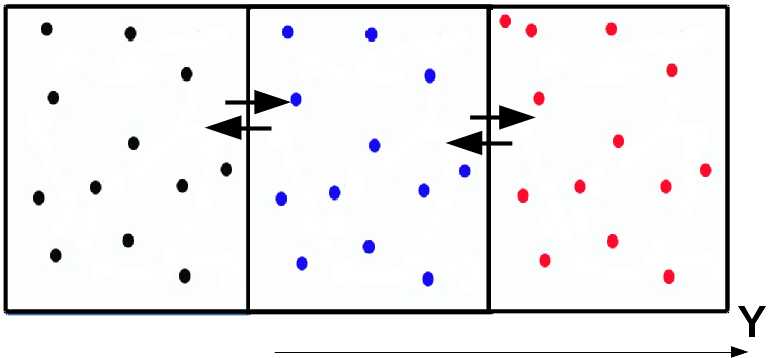
\includegraphics[height=4cm,keepaspectratio]{images/decomp_Eu.png}
	\end{center}
	\caption{Эйлерова декомпозиция расчетной области. На рисунке показано разделение расчетной области на подобласти вдоль одной из координат. Точки разных цветов показывают модельные частицы, находящиеся на разных процессорных  элементах. Маленькие черные стрелки означают обмен граничными значениями полей и токов между подобластями. Используются парные операции MPI (MPI\_Send и MPI\_Recv).}
	\label{Lag_dec}
\end{figure}





\begin{table}[ht]
\begin{center}
\caption{Эффективность в слабом смысле, достигнутая при различных вариантах декомпозиции.}
\begin{tabular}{|c|c|c|}
\hline
Декомпозиция & тип коммуникаций        &  эффективность (МСЦ РАН) \\
             &                         &  на 100 ПЭ\\ \hline
эйлерова     & <<точка-точка>>         &   77 \%  \\ \hline
 лагранжева  & коллективные            &   15 \%  \\
             &  по всем ПЭ             &        \\ \hline
 смешанная   & <<точка-точка>> и       &   92 \%  \\ 
             & коллективные            &       \\
             & по небольшим            &        \\ 
             & группам ПЭ              &      \\ \hline 
\end{tabular}
\end{center}
\end{table}


\begin{figure}[ht]
	\begin{center}
		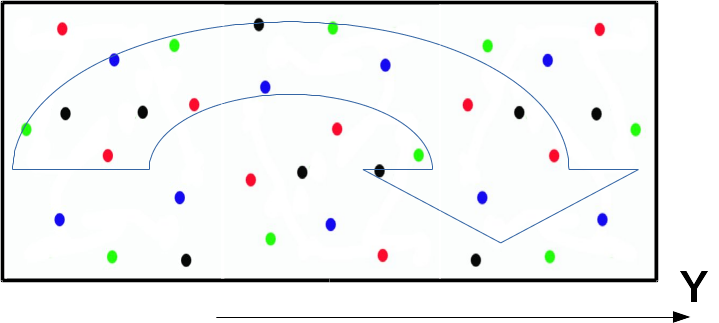
\includegraphics[height=4cm,keepaspectratio]{images/decomp_Lag.png}
	\end{center}
	\caption{Лагранжева декомпозиция расчетной области. Геометрически область не разделяется на подобласти. Точки разных цветов показывают модельные частицы, находящиеся на разных процессорных  элементах. Большая полая стрелка означает сборку значений тока, вычисленных каждым ПЭ по имеющимся у него частицам. Используются коллективные операции MPI (MPI\_Allreduce)}
	\label{Euler_dec}
\end{figure}




%\subsubsection{Декомпозиция расчетной области}



Для параллельной реализации метода частиц в ячейках в данной работе используется эйлерово-лагранжева декомпозиция расчетной области. Такой вариант выбран из соображений наилучшей масштабируемости вычислительного алгоритма.
При этом расчетная область разделяется на подобласти для решения уравнений Максвелла, и на каждую подобласть назначается группа из $M$ ПЭ, далее частицы каждой подобласти разделяются дополнительно между этими $M$ ПЭ. Такой вариант декомпозиции одновременно обеспечивает минимизацию фрагмента вычислительного алгоритма и также соответствует условию линейности алгоритма, необходимому для достижения высокой масштабируемости. Этот подход близок к виртуальным слоям (Malyshkin, Kraeva, 2001).



Наилучшим достигнутым результатом в рамках диссертационной работы является эффективность в слабом смысле 92 \%, полученная на суперкомпьютере <<Ломоносов>>, НИВЦ МГУ с использованием 500 графических ускорителей Nvidia Tesla. 
В пользу именно такого, смешанного варианта декомпозиции можно высказать следующие теортические соображения:
\begin{itemize}
	\item Для эйлеровой декомпозиции минимальным фрагментом (Понятие минимального фрагмент было введено В.Э.Малышкиным, 2001) является слой сетки вместе с частицами
	\item Для лагранжевой декомпозиции минимальный фрагмент - одна частица
	\item Тем не менее, для лагранжевой декомпозиции (из-за необходимости осуществлять коллективные коммуникации по всем ПЭ) нарушается критерий линейности алгоритма (В.Э.Малышкин, 1991)
	\item Эйлерово-лагранжева декомпозиция позволяет одновременно минимизировать размер фрагмента и обеспечить линейность
	
\end{itemize}

{\small Снытников А.В."Моделирование на суперЭВМ аномальной  теплопроводности в плазме термоядерной ловушки"// Труды всероссийской суперкомпьютерной конференции <<Научный сервис в сети Интернет: масштабируемость, параллельность, эффективность>>, 21-26 сентября \textbf{2009}}


\begin{figure}[ht]
\begin{center}
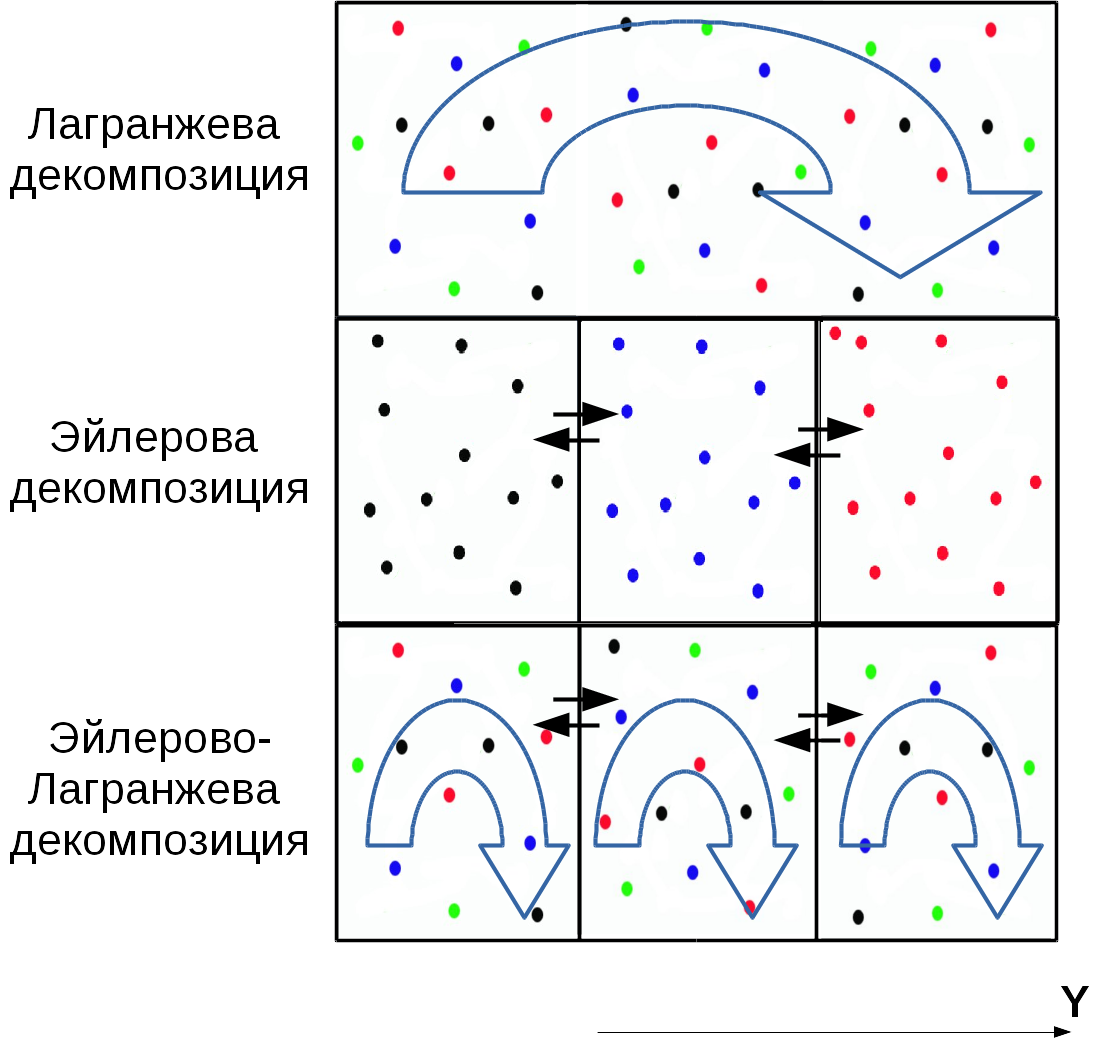
\includegraphics[height=10cm,keepaspectratio]{images/decomp_all.png}
\end{center}
\caption{Сравнение всех рассмотренных видов декомпозиции.На рисунке показано разделение расчетной области на подобласти вдоль одной из координат. Точки разных цветов показывают модельные частицы, находящиеся на разных процессорных  элементах. Маленькие черные стрелки означают обмен граничными значениями полей и токов между подобластями. Большая полая стрелка означает сборку значений тока, вычисленных каждым ПЭ по имеющимся у него частицам. Используются как  парные (MPI\_Send и MPI\_Recv), так и коллективные операции MPI (MPI\_Allreduce).}
\label{decomp_all}
\end{figure}



\clearpage

\section{Ход вычислений в программе}


\section{Программная реализация вычислительных методов}
   В этом разделе подробно описывается ход вычислений в программе-тесте, созданной в рамках диссертационной работы. Несмотря на то, что ни сами вычислительные методы, ни их программная реализация не являются основным содержанием диссертации, и не входят в положения, выносимые на защиту, тем не менее необходимо максимально точно описать, что входит в программу-тест, запускаемую на ВС для того, чтобы было видно, какая нагрузка создается на различные подсистемы ВС и в частности, для того, чтобы определить объем вычислений (количество операций с плавающей точкой) на каждую модельную частицу, количество данных в оперативной памяти, и объем пересылок.
   
   
\subsection{Вычисление электромагнитного поля во всей расчетной области}

\begingroup
\captiondelim{ } % разделитель идентификатора с номером от наименования
\lstinputlisting[lastline=49,language={[ISO]C++},caption={Функция, выполняющая расчет одной из компонент электрического поля в отдельном узле сетки.},label={list:eme}]{listings/emeElement.cxx}
\endgroup 
Непосредственно на листинге \ref{list:eme} можно увидеть 7 операций с плавающей точкой. Эта функция вызывается $N_X \times N_Y \times N_Z$ раз для каждой из трех компонент электрического поля, всего 
$21 N_X \times N_Y \times N_Z$ операций.

\begingroup
\captiondelim{ } % разделитель идентификатора с номером от наименования
\lstinputlisting[lastline=49,language={[ISO]C++},caption={Функция, выполняющая первый этап расчета одной из компонент магнитного поля в отдельном узле сетки.},label={list:emh1}]{listings/emhElement.cxx}
\endgroup 

 Аналогично, на листинге \ref{list:emh1} видно 7 операций с плавающей точкой. Эта функция также вызывается $N_X \times N_Y \times N_Z$ раз для каждой из трех компонент магнитного поля, всего 
 $21 N_X \times N_Y \times N_Z$ операций.

\begingroup
\captiondelim{ } % разделитель идентификатора с номером от наименования
\lstinputlisting[lastline=49,language={[ISO]C++},caption={Функция, выполняющая второй этап расчета одной из компонент магнитного поля в отдельном узле сетки.},label={list:emh2}]{listings/emh2Element.cxx}
\endgroup 
   
И листинг \ref{list:emh2} добавляет еще одну операцию. Эта функция также вызывается $N_X \times N_Y \times N_Z$ раз для каждой из трех компонент магнитного поля, всего 
$3 N_X \times N_Y \times N_Z$ операций.

В итоге вычислительная нагрузка при вычислении электромагнитного поля составляет $45 N_X \times N_Y \times N_Z$ операций.
   
  
   
\subsection{Расчет электромагнитного поля в точке нахождения модельной частицы}
На листинге \ref{list:interpolate} показана функция, интерполирующая значения электромагнитного подя из узлов ячейки в точку нахождения частицы. Как видно из листинга, поля и частицы хранятся внутри ячейки, а не в виде одного глобального массива, содержащего значения поля во всей области. Подход с хранением полей и частиц в виде глобальных массивов также был реализован, и важно отметить, что при этом возникает существенная разница по производительности. Эта разница подробно исследуется в 3-й главе (раздел \ref{procs_influence}) и обычно составляет до 200 \%. Таким образом для программы-теста можно использовать как тот, так и другой подход, внося соотвествующую поправку в полученные результаты.
   
\begingroup
\captiondelim{ } % разделитель идентификатора с номером от наименования
\lstinputlisting[lastline=49,language={[ISO]C++},caption={Расчет электромагнитного поля в точке нахождения модельной частицы},label={list:interpolate}]{listings/interpolate.cxx}
\endgroup 
интерполяционные коэффициенты, задаваемые в качестве параметров функции Interpolate, вычисляются в функции InverseKernel, реализующей операцию, обратную по отношению к ядру модельной частицы:

\begingroup
\captiondelim{ } % разделитель идентификатора с номером от наименования
\lstinputlisting[lastline=32,language={[ISO]C++},caption={Вычисление инетерполяционных коэффициентов},label={list:inverse}]{listings/inverse.cxx}
\endgroup    

\subsection{Расчет движения модельной частицы}
В этом разделе показан листинг функции, рассчитывающей движение модельной частицы, то что в зарубежной литературе именуется particle pusher. Следует отметить, что это наиболее важная с точки зрения производительности и наиболее вычислительно нагруженная часть программы.

\begingroup
\captiondelim{ } % разделитель идентификатора с номером от наименования
\lstinputlisting[lastline=79,language={[ISO]C++},caption={Интегрирование уравнений движения модельной частицы},label={list:inverse}]{listings/push.cxx}
\endgroup   
 
Цель демонстрации всех перечисленных фрагментов программного кода, заключается в том, чтобы можно было подтвердить оцекнку количества операций с плавающей точкой, затрачиваемых на одну модельную частицу в течение одного временного шага: 500 операций. Это число будет в дальнейшем использоваться для определения производительности вычислительных систем и в ччастности, их процессорных ядер во флопсах (FLOPS).  


\section{Список входных и выходных данных программы}	

Входные данные:
\begin{itemize}
\item Размер сетки
\item Количество процессоров
\item Количество частиц в ячейке
\item Размер области
\item Размер части области, занятой пучком и плазмой
\item Внешнее магнитное поле
\item Энергия частиц пучка
\item Поперечная температура частиц пучка
\item Температура плазмы (X,Y,Z)
\end{itemize}

Выходные данные (опционально, каждая выдача может быть отключена):
\begin{itemize}
\item Списки модельных частиц (координаты, импульсы)
\item Плотности электронов, ионов и электронов пучка
\item Электрическое и магнитное поля (все три компоненты)
\item Ток (три компоненты)
\item Одномерная функция распределения электронов (всех, и пучка, и плазмы) по энергии
\end{itemize}

С точки зрения тестирования ВС основное значение имеют следующие выдачи (отдельно для каждого MPI-процесса):

\begin{enumerate}
	\item Средняя продолжительность операций MPI, причем по отдельности для разных объемов пересылаемых данных и разных стадий вычислительного алгоритма:
	\begin{itemize}
		\item MPI\_Send/Recv - пересылка граничных значений поля и пересылка частиц
		\item MPI\_Allreduce - сложение значений тока в подобласти при лагранжевой декомпозиции
		
	\end{itemize}	
	\item Время пересылки частиц, граничных значений поля, время сборки данных при выполнении коллективных операций   
	\item Время выполнения каждой отдельной стадии вычислительного алгоритма:
	\begin{itemize}
		\item расчет поля, 
		\item пересылка граничных значений, 
		\item расчет движения частиц, 
		\item пересылка частиц в соседние процессоры, 
		\item сборка значений тока при лагранжевой декомпозии
	\end{itemize}
	\item Время записи файлов на диск 
	\item Время копирования данных на GPU и обратно
	
\end{enumerate}

Реализованная в диссертационной работе тестовая программа получила условное наименование 
PIC-MANAS (Particle-In-Cell Multi-Archtitecture Numerical Analysis \& Simulation).

           % Глава 1
%\chapter{Физико-математические задачи и вычислительные методы в исследованиях, проводимых с использованием высокопроизводительных ВС} \label{chapt2}
В последние годы (с 2010 по 2016 год) было опубликовано много статей (более 300) в различных международных журналах по тематике <<экзафлопсные вычисления>> (т.е. вычисления на перспективных ВВС производительностью порядка $10^{18}$ операций с плавающей точкой в секунду), из них около трети посвящены решению различных прикладных задач.
Данные обзора отдельными частями опубликованы в \cite{MohographyTarkov,VestnikNNSU,multigridAuto,AutoParSilan,VychMetPlasma,Adaptive,VestnikNSU3D,NumMethMultiLevel,MatMod,VestnikNSUadapt,VychMethProgExa,SuperFrI,adaptCPC,LotovPoP,astroCoDesign,integrApproach}.

В обзорную часть данной диссертационной работы вошло 298 статей, в том числе 110 статей посвящено различным физическим приложениям экзафлопсных вычислений, распределение статей по физическим приложениям показано в таблице \ref{tab_physics}.


\begin{table}[ht]
	\caption{Распределение по приложениям статей относящихся к тематике <<экзафлопсные вычисления>>}
	\begin{center}
		\begin{tabular}{|c|c|}
			\hline
			вычислительная гидродинамика & 27  \\ \hline 
			ядерные технологии & 17       \\ \hline  
			физика плазмы & 11  \\ \hline 
			разработка новых материалов & 10  \\ \hline 
			предсказание погоды & 10 \\ \hline 
			биомедицинские приложения & 9 \\ \hline 
			астрофизика и космология & 6  \\ \hline 
			молекулярная динамика   & 6   \\ \hline 
			мультифизика & 6              \\ \hline 
			геофизика & 6  \\ \hline 
			финансы & 2  \\ \hline 
		\end{tabular}
	\end{center}
	\label{tab_physics}
\end{table}

Как видно из таблицы \ref{tab_physics} особенно активно математическое моделирование используется в следующих областях науки и техники.  
\begin{itemize}
	\item Гидродинамика (космическая газодинамика, расчет обтекания кораблей и самолетов, например, из числа статей, относящихся к пета- и экзафлопсным вычислениям, \cite{Onishi2014},\cite{Lu2015,Peterson1989}, предсказание наводнений в прибрежных городах Северной Европы и другие экологические вопросы, моделирование океанических течений \cite{STERN20151,Newman20152086,Reuter2015325,Walker2014287}, расчет гидродинамической турбулентности %\cite{BirdsallIEEE}%
	\cite{Mininni2011316,Appeloe201019,Yokota2013445,Tucker2016,Kotov2016189}  моделирование многофазных течений \cite{Safi2016170,Zaspel2016505}, построение сеток для гидродинамического моделирования \cite{Shang2013381,Yilmaz2013388,Ono20142336,Yilmaz2013773}),
	\item Ядерные технологии, точнее моделирование различных процессов, протекающих в ядерных реакторах. \cite{Romano2013274,Romano201320,Romano201590,Boyd201443,Gong2012588,Gong20116010,Bergmann2015176,Bauge201432}, 
	\item Разработка новых материалов (квантовохимические расчеты структуры и поведения молекул, вычисление супер-многомерных интегралов в различных приближениях \cite{Ono2015}), методы молекулярной динамики \cite{Valiev20101477,Aguilar20132197,Yokota201317,Ohno20142575,Xu2015200}
	\item Моделирование ускорителей заряженных частиц \cite{Silva2014229}, 
	\item Плазменные технологии\cite{BirdsallIEEE}
	\item Плазменные процессы в установках управляемого термоядерного синтеза
	\cite{KatesHarbeck2016231,Winkel2015456,Minoshima201381,Kumar20132251,Decyk2014,Acebron2013224}. 
	\item Разработка новых лекарств и другие биомедицинские приложения \cite{Stone2015,Joshi2011200,Saraladevi2015596,Blau20132856,Wang2012254,Markram201139,Markowitz2015730} (наибольшее количество расчетов с использованием большого количества процессоров, производилось именно в этой области). 
	
	\item Также математические модели для пета-и экзафлопсных ВВС создаются в геофизике \cite{Christen2012956,Nakajima20131265,Zhong2015197,Reed20131,Hodges201316,Furumura20111448}.
\end{itemize}

С учетом того, что во многих областях приходится иметь дело с несколькими различными и одновременно протекающими физическими процессами при этом эти различные процессы моделируются совершенно различными способами, существует необходимость разработки высокомасштабируемого программного обеспечения для таких приложений, которые в зарубежной литературе называются мультифизическими (multiphysics). Это делается в работах \cite{Yamamoto2014576,Agullo201196,Ettrich20151,Vazquez2016,
	Liu2011261,Zheng2015313}.

Наиболее существенной областью приложений пета- и экзафлопсных вычислений оказались ядерные технологии и вопросы моделирования ядерных реакторов (статей, посвященных вычислительной гидродинамике, больше, как видно из таблицы \ref{tab_physics}, но это очень обширная и разнообразная область). В основном разрабатываются масштабируемые версии методов Монте-Карло для переноса нейтронов \cite{Romano2013274,Romano201320,Romano201590,Boyd201443,Gong2012588,Gong20116010,Bergmann2015176,Bauge201432}, проводится анализ коммуникационных потерь в методе Монте-Карло \cite{Siegel20123119,Horelik2014646,Tramm2016}. Также рассматриваются вопросы взаимодействия пучков частиц с материалами \cite{Bandura20103485} и применение решеточных уравнений Больцмана с использованием квантовой хромодинамики к задачам ядерной физики\cite{Beane20111,Savage2012140}.
Следует особенно отметить работы по созданию интегральной среды для разработки ядерных реакторов \cite{Patterson201697} и моделирование новых видов реакторного топлива \cite{Stan200920}.

Разработка технологии решения физических задач с помощью современных и перспективных высокопроизводительных ЭВМ составляет содержание диссертационной работы. Использование ВВС будет показано на примере решения задач динамики плазмы, аналогичных, рассмотренным в \cite{BretPoP2010,BirdsallIEEE,LangdonBirdsall}. Эти задачи представляют чрезвычайно большой научный интерес, а также очень актуальны с точки зрения использования результатов моделирования в промышленности. Такой выбор не ограничивает общности полученных в данной работе результатов, так как разработанные технологии использования ВВС могут быть применены также и в других областях, в особенности в гидродинамическом и в квантовохимическом моделировании.

В частности, одной из важных областей приложения созданных методов оказывается сейсмология, при использовании метода частиц
\cite{hockney,VshivkovPICbook} как альтернативы решению уравнения эйконала \cite{Engquist}.

Плазменные задачи представляют большой интерес как с точки зрения выбора и обоснования модели (равновесная плазма или неравновесная, устойчивая или неустойчивая, магнитогидродинамическое описание или кинетика), так и с точки зрения  вычислительных методов (решение уравнения Пуассона или уравнений Максвелла, выбор одного из многих вариантов решения кинетического уравнения или уравнений МГД), и в особенности с точки зрения разработки и программной реализации вычислительных алгоритмов (различные варианты декомпозиции расчетной области, организации межпроцессорных обменов, достижения оптимальной производительности), т.е. плазменные задачи требуют поиска новых решений на всех уровнях триады Академика А.А.Самарского: <<модель, алгоритм, программа>> \cite{SamarskiMatMod}.  

Все перечисленные вопросы в том или ином виде встречаются и в других областях математического моделирования, тем не менее в физике плазмы есть проблемы, не имеющие аналога по степени сложности (и соответственно, по количеству необходимых для решения вычислительных ресурсов). Эти проблемы возникают при моделировании плазменных неустойчивостей и турбулентностей в установках управляемого термоядерного синтеза (УТС) при высоких температурах (1-5 КэВ, что соответствует 10 млн.градусов), когда плазма не является даже приближенно равновесной в сколь угодно малой окрестности. В этом случае плазма имеет очень большое количество степеней свободы \cite{MohographyKhoroshevsky}, необходимость учета которых приводит к использованию соответствующих больших объемов памяти.

Особенная важность решения задачи о динамике плазмы в установках УТС связана с тем, что управляемый термоядерный синтез является единственным вариантом решения энергетической проблемы. Все существующие альтернативные энергетические концепции имеют очень серьезные недостатки, не позволяющие рассматривать их как решение энергетической проблемы в мировом масштабе: углеводородная энергетика имеет ограниченные запасы топлива, атомная энергетика представляется экологически опасной, электростанции на солнечной энергии не могут строится из-за (возможно, временной) дороговизны и экологических проблем, возникающих при производстве фотоэлементов в больших количествах, а различного рода <<экологически чистые>> электростанции, такие как ветряные, приливные, геотермальные не могут строится в необходимых больших количествах, также, как и крупные ГЭС.

Другая важная область приложения моделирования плазмы - это промышленные плазменные технологии, используемые, в частности, для производства чистого кремния для нужд микроэлектронной промышленности и для производства микропроцессоров (установки молекулярно-лучевой эпитаксии). Также моделирование высокотемпературной плазмы может быть полезно для исследования природы солнечных вспышек и исследования их влияния на магнитосферу Земли и арктическую навигацию \cite{RussellIEEE}.
	
Подводя предварительный итог, нужно подчеркнуть еще раз, что применение современных высокопроизводительных ЭВМ может дать качественный скачок в решении многих важных научных и производственных задач. Далее необходимо дать краткое описание этих ЭВМ с тем, чтобы определить стратегию их использования. 

На конференциях по высокопроизводительным вычислениям \cite{Abrau2011} широко обсуждались вопросы связанные с построением экзафлопс-компьютеров и трудностями создания программного обеспечения для них. 
В первую очередь это чрезвычайно большое ожидаемое энергопотребление - порядка 1 ГВт. Таким образом, на первый план выходят вопросы эффективной эксплуатации такой исключительно дорогой машины, а энергоэффективность алгоритма становится определяющей чертой для допуска этого алгоритма к расчетам.

Ограничивая мир высокопроизводительных вычислений первой десяткой наиболее мощных ВС мира, а это вполне оправдано в том случае, если речь идет о возможной архитектуре экзафлопс-компьютера,  можно сказать, что этот мир весьма неоднороден. Серьезно отличаются базовые элементы, на основе которых строятся ВВС , как процессоры (Intel Xeon, AMD Opteron, Sun UltraSPARC), так и ускорители вычислений (Intel Xeon Phi, Nvidia Kepler). 

С учетом того, что наиболее мощные компьютеры строятся ( вероятнее всего и дальше будут строиться \cite{Lu2015}) на основе ускорителей вычислений \cite{Stepanenko2010}, для эффективного использования компьютеров большой мощности с целью решения актуальных физических задач принципиально необходимо значительно упростить освоение гибридных (т.е. построенных с использованием как процессоров общего назначения, так и ускорителей вычислений) ВВС с точки зрения специалиста по моделированию в конкретной предметной области или физика. 

Описанное разнообразие архитектур означает, что все реализации вычислительных алгоритмов для перспективных экзафлопс-компьютеров должны быть в достаточной степени универсальными, чтобы иметь возможность проводить расчеты на тех процессорах или ускорителях вычислений, которые будут  выбраны для создания экзафлопс-компьютера, в частности, на всех перечисленных типах вычислительных устройств. 


Кроме того, следует отметить широко обсуждаемые трудности создания программного обеспечения для экзафлопсных ВВС, связанные с наличием в составе этих ВВС сотен тысяч и миллионов процессорных элементов. По данному вопросу существует две противоположных точки зрения. 
Согласно одной из них, для эффективной работы на экзафлопсных ВВС потребуется создание принципиально новых математических основ вычислительной техники, операционных систем, языков программирования и пр., не требующих межпроцессорных коммуникаций в принципе. Другая точка зрения заключается в том, что решение задач на экзафлопсных ВВС будет производится с использованием существующего программного обеспечения, т.е коммуникационных библиотек, основанных на сообщениях \cite{Gropp2009} и алгоритмических языках программирования. 

Таким образом, можно строить реализацию вычислительных алгоритмов для 
экзафлопсных ВВС на основе модели передачи сообщений (самый известный ее вариант называется MPI) и исходя из предположений об иерархической структуре коммуникационной системы.
Наиболее важным вопросом реализации вычислительного алгоритма на ВВС является вопрос масштабируемости алгоритма, то есть обеспечение равномерной загрузки процессорных элементов - отдельных процессоров, ускорителей вычислений или узлов суперкомпьютера.  

Одним из наиболее эффективных принципиальных подходов к созданию эффективных параллельных алгоритмов является сборочная технология параллельного программирования \cite{MalyshkinSynthesis,MalyshkinASSY,Kraeva2001,
	MalyshkinTsigulin}, согласно которой параллельная программа собирается из множества   готовых атомарных фрагментов, содержащих как данные, так и алгоритмы.

Существует множество подходов, используемых для достижения более высокой производительности, 
\begin{itemize}
	\item декомпозиция расчетной области\cite{Liewer1989,Kraeva2001,Stijnman2003, Eastwood1995}, с целью ее разделения на более мелкие подобласти, 
	\item использование большого количества процессорных элементов (разработка системного программного обеспечения, позволяющего увеличить число ПЭ сверх определенного предела
	\cite{Gropp2009} или создание численных методов с меньшим количеством необходимых коммуникаций)
	\item применение многоядерных процессоров или различных ускорителей вычислений \cite{SteYuz13}. позволяющих увеличить скорость счета без возрастания нагрузки на коммуникационную сеть, оптимизация под архитектуру процессора или ускорителя, 
	\item сокращение количества отправляемых сообщений, 
	\item переход к численным методам, более подходящим для многопроцессорных ЭВМ (от неявных схем к явным, к методам на основе ортогональных преобразований. от методов, рассматривающих объект моделирования как сплошную среду к методам частиц и пр.) или численных методов специально подобранных или специально оптимизированных для решения конкретной задачи. 
\end{itemize}

Однако все перечисленные подходы можно разделить на три принципиально разных непересекающихся направления:
\begin{itemize}
	\item увеличение числа ПЭ (процессорных элементов)
	\item адаптация вычислительных методов к архитектуре ВВС
	\item использование ускорителей вычислений 
\end{itemize}

С этой точки зрения был проведен обзор недавних (2010-2016 годы) публикаций, относящихся к тематике <<экзафлопсные вычисления>> в журналах Future Generation Computer Systems, Procedia Computers Science, Journal of Parallel and Distributed Computing, Parallel Computing, Journal of Computational Physics, Computer Physics Communications и др.
По трем указанным выше направлениям они распределились, как показано на рисунке \ref{exaflops_topics_fig}.


 	\begin{figure}[htb]
 		 \begin{center}
 		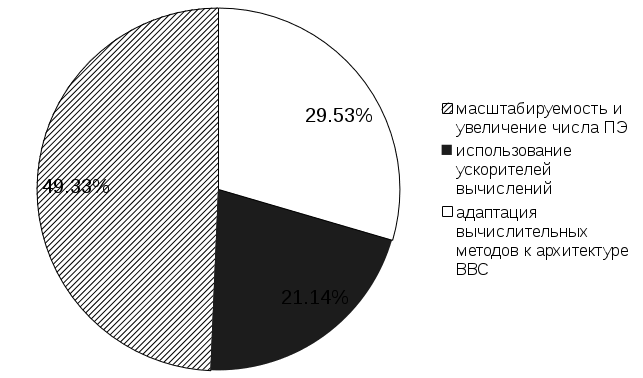
\includegraphics[height=7cm,keepaspectratio]{images/exaflops_topics_15.png}
 		\caption{Распределение по направлениям статей относящихся к тематике <<экзафлопсные вычисления>>}
 		\label{exaflops_topics_fig}
 		 \end{center}
 	\end{figure}
 %\end{center}




\begin{table}[ht]
\caption{Распределение по направлениям статей относящихся к тематике <<экзафлопсные вычисления>>}
\begin{center}
\begin{tabular}{|c|c|c|}
\hline
Условное наименование направления      & Число статей & В \%  от     \\
                                       &              & общего числа \\ \hline
масштабируемость и увеличение числа ПЭ & 147 &          49 \\  \hline
использование ускорителей вычислений   & 63  &          21 \\  \hline
адаптация вычислительных методов       & 88  &          30  \\ 
к архитектуре ВС                       &     &              \\ \hline  
\end{tabular}
\end{center}
\label{exaflops_topics_tab}
\end{table}

\section{Масштабируемость и увеличение числа ПЭ}

 \begin{table}[ht]
 	\caption{Распределение по темам статей относящихся к направлению
 		<<масштабируемость и увеличение числа ПЭ>>}
 	\begin{center}
 		\begin{tabular}{|c|c|c|}
 			\hline
 			Тема                       & Количество          & В \%           \\
 			& статей в обзоре     & от общего числа (от 298 статей)  \\ \hline 
 			масштабируемые                 & 27 & 7.04  \\    
 			архитектуры                    &    &       \\   \hline
 			программные средства           &    &       \\
 			для повышения                  &    &       \\
 			масштабируемости              & 18 & 6.04  \\ \hline 
 			Ускорители и                   &    &      \\
 			специальное оборудование       &    &      \\
 			для повышения                  &    &      \\
 			масштабируемости              & 14 &  1.37 \\ \hline 
 			Моделирование                  &    &     \\
 			функционирования               &    &     \\
 			экзафлопсных систем            & 19 & 6.38  \\ \hline 
 			Упрощение работы с             &    &          \\
 			экзафлопсными системами       & 11 & 3.69 \\ \hline 
 			Декомпозиция                   &    &	      \\
 			расчетной области             & 10 &  3.36 \\ \hline 
 			Динамическая                   &    &       \\
 			балансировка загрузки          & 24 &  8.05 \\ \hline 
 			Отказоустойчивость             & 20 & 6.71  \\ \hline 
 			Уменьшение                     &    &        \\
 			количества коммуникаций        & 10 & 3.36   \\ \hline 
 		\end{tabular}
 	\end{center}
 	\label{topic_maxPE}
 \end{table}
 
 
 Первое направление, названное условно <<масштабируемость и увеличение числа ПЭ>> было, в свою очередь, разделено
 на несколько тем, как показано в таблице \ref{topic_maxPE}. Смысл этой таблицы заключается в том, чтобы очертить круг задач, которые должны решаться с помощью разрабатываемого в данной работе тестового приложения для высокопроизводительных вычислительных систем. Таким образом, если некоторому вопросу уделяется существенное внимание при разработке программного обеспечения для перспективных ВС, например, динамической балансировке загрузки, то создаваемый тест должен быть способен в том или ином виде ответить на вопрос, насколько эффективно может быть реализована динамическая балансировка на конкретной ВС, чья производительность анализируется в помощью разработанного в данной работе теста.
 При этом количество статей или их доля в обзоре, указанная в таблице  \ref{topic_maxPE}, является приближенным наукометрическим показателем важность конкретной тематики.
 
  При этом значение имеет только лишь сам факт наличия публикаций по некоторой теме, количество их не имеет принципиального значения, если только оно не очень велико, в силу того что статистическая погрешность приведенных показателей в процента равна $1/\sqrt{300} \approx 6 \%$.
  Таким образом лишь в том случае можно говорить, что по некоторой теме опубликовано больше статей, чем по какой-то другой, когда разница по количеству статей не менее чем 18-20 работ. 
  
  Это же относится и к другим таблицам 2-й главы: важен во-первых, сам факт упоминания некоторой тематики в исследованиях по достижению экзафлопсной производительности, и во вторых, имеет значения лишь значительная разница по количеству статей, написанных на ту или другую тему (более чем на 6 \%).
 \clearpage
 
 К теме <<масштабируемые архитектуры>> были отнесены такие работы, как, например, алгоритм привязки процессов к узлам на коммуникационной сети ВВС в виде трехмерного тора \cite{Kodama2014362},
 метаматематические основы проектирования бесконечно расширяемых машин на основе идеальной модельной архитектуры \cite{Anderson20151828}, опыт эксплуатации и решения задач на машине K computer (№ 4 в списке Top500 за ноябрь 2015), имеющей хорошие характеристики масштабируемости и, в отличие от № 1 и № 2, построенной не на основе ускорителей вычислений \cite{Yamamoto2014576}. Также к этой теме отнесена работа, посвященная использованию большого количества ядер в программах, написанных для старых компьютерных архитектур: несмотря на то, что работа посвящена программированию, основные вопросы, которые там решаются - это архитектурные вопросы, точнее преодоление архитектурных различий программными средствами \cite{Lohner201353}.
 
 К теме <<программные средства для повышения масштабируемости>> отнесены разработки коммуникационного программного обеспечения, например, MPI, специально предназначенного для работы с очень большим количеством процессов \cite{Zounmevo2014265}, или механизмы снижения задержки сообщений в MPI \cite{Khunjush2009430}. Также к этой теме относится создание высокомасштабируемых пакетов программ для решения конкретных задач \cite{Valiev20101477,Peng20131469}.
 
 Следующая тема, <<Ускорители и специальное оборудование для повышения масштабируемости>>, образована такими работами, как исследование масштабируемого ввода-вывода на кластере из ПЛИС (программируемых логических интегральных схем) \cite{Schmidt2012344}. Следует отметить, что к этой теме не относятся вопросы конструирования кластеров на ПЛИС и соответствующие проблемы программирования, а только лишь влияние необычного оборудования (в частности ПЛИС) на масштабируемость. Кроме того, к этой теме отнесены исследование поведения закона Амдала \cite{Amdahl} на многоядерных системах \cite{Yavits2014} и разработка специализированного сетевого оборудования типа <<сеть на кристалле>>  \cite{Khanjari2015403}, а также создание
 сопроцессоров для диспетчеризации потоков \cite{Giorgi2015100}.
 
 В связи с отсутствием реально функционирующих ВС экзафлопсного класса, а также в связи с предполагаемой исключительной дороговизной вычислительного времени на этих системах, особенную важность приобретает тема  <<Моделирование функционирования экзафлопсных систем>>, включающая в себя также	 и моделирование работы прикладных программ на этих системах. К этой теме относятся анализ расхода времени на коммуникации \cite{Siegel20123119} и подбор с помощью моделирования оптимального (по коммуникациям) варианта декомпозиции расчетной области \cite{Hag2015400}, а также моделирование и предсказание аварийных ситуаций \cite{Aupy20142048}.

 В докладе профессора Н.Н.Миренкова на конференции Parallel Computing Technologies-2009 (PaCT-2009) \cite{Watanobe2009} была высказана точка зрения о том, что на новые поколения ВВС (гигафлопсные, терафлопсные, петафлопсные,...) раз за разом возлагались очень серьезные надежды на прогресс в решении реальных физических задач, тем не менее реальные успехи могут быть охарактеризованы лишь как очень скромные. Причина этого, по мнению Н.Н.Миренкова \cite{Watanobe2009} заключается в том, что специалисты в конкретной предметной области не понимают, как можно использовать ВВС, и не видят смысла в их использовании. Возможный выход заключается в создании удобных, интуитивно понятных инструментов для создания программ на ВВС. Такие работы активно ведутся, и в рамках настоящего обзора они выделены в тему <<Упрощение работы с  экзафлопсными системами>>. Сюда относятся создание учебников по конструированию и эксплуатации кластеров \cite{Georgi20111917}, разработка средств отладки параллельных приложений \cite{Jin20131774,Huenich20151383}, а также создание новых средств администрирования \cite{Gallard2012136}.
 
 Важнейшим вопросом для обеспечения высокой масштабируемости при решении конкретных задач является декомпозиция расчетной области. К этой теме отнесены работы, в которых основное внимание уделяется изначальному распределению загрузки, т.е. без динамики, а также те работы, в которых предлагается оптимизация доступа к данным независимо от их распределения в рамках вычислительной системы \cite{Srinivasa2012256},\cite{Lieb2014246}, или разрешение конфликтов при распределении различных видов данных, с различными вариантами доступа к ним, например, \cite{Sitaraman2016,Balzuweit201667}.

В отличие от предыдущего пункта, к теме <<Динамическая балансировка загрузки>> отнесены вопросы оптимизации загрузки процессорных элементов, проводимой во время работы программы, например, исследование воздействия несбалансированности загрузки на производительность методов Монте-Карло \cite{Siegel2013901} или реализация метода частиц в ячейках с динамической балансировкой загрузки на языке parallel C \cite{Verleye201310}, а также вопросы, связанные с балансировкой загрузки не только прикладной программы, но и вычислительной системы в целом, что особенно важно с точки зрения перспективы экзафлопсных вычислений \cite{Dong20121254}.



Следующая тема, <<отказоустойчивость>>, исключительно важна для подготовки к вычислениям на экзафлопсных машинах,
с учетом того, что различного сорта ошибки будут происходит на системах, состоящих из миллионов процессоров практически каждую секунду. Кроме того, стоимость проведения таких расчетов, как ожидается, будет очень высокой (сейчас расчет продолжительностью в 10 млн. процессоро-часов с использованием метода частиц в ячейках оценивается в 0.5 млн. евро \cite{Vieira}). К этой теме относятся
обработка контрольных точек, оптимизация и ускорение их чтения и записи \cite{Nicolae2013698,Casanova20157}, диспетчеризация процессов с учетом наличия поврежденных или вышедших из строя процессорных элементов \cite{Defour20161},
а также анализ производительности реализации MPI, работающей с учетом наличия в системе сбоев \cite{Hursey201215}.

К последней теме (<<уменьшение количества коммуникаций>>) в рамках направления <<масштабируемость и увеличение числа ПЭ>> отнесены статьи, посвященные созданию параллельных алгоритмов, стремящихся к минимуму коммуникаций (англ. communication-avoiding \cite{Dongarra2013212}). Важность этой темы очевидна для экзафлопсных вычислений: при наличии миллионов процессорных элементов, обменивающихся сообщениями, количество сообщений оценивается (минимально), как $O(N)$, где $N$ - число процессоров, поэтому очень важна разработка алгоритмов, способных или вовсе обойтись без коммуникаций или снизить их количество до $O(1)$. К таким алгоритмам относятся: метод решёточных уравнений Больцмана \cite{Wittmann2013924,Safi2016170}, а также, разработка модели свободной поверхности океана с минимизацией объема коммуникаций\cite{Newman2016877} или решение уравнений типа уравнения Пуассона алгебраическим многосеточным методом, масштабируемым в том смысле, что время решения пропорционально количеству неизвестных (а не количеству ПЭ) \cite{Notay2015237}.

\section{Адаптация вычислительных методов к архитектуре ВВС}

Второе направление работ над экзафлопсными вычислениями, выделенное в рамках обзора, названо <<адаптация вычислительных методов к архитектуре ВВС>>. 

Сюда относятся численные методы, разработанные специально для экзафлопсных машин (методика локального сгущения шага при решении уравнений реакции-диффузии \cite{Krause2016164}, решение дифференциальных уравнений в частных производных с пониженным объемом коммуникаций \cite{Norman2015}).
Другая тема  - адаптация имеющихся численных методов для работы на очень большом количестве ПЭ (например, вариант итерационного метода Якоби с ускорением Андерсона \cite{Pratapa201643} или масштабируемые алгоритмы Монте-Карло для финансового моделирования \cite{Alexandrov20111708}). Здесь необходимо ответить на вопрос: где проходить грань между алгоритмами, специально разработанными для экзафлопсных машин, и алгоритмами, адаптированными для экзафлопса. Казалось бы, разница незначительна, и более того, поскольку то, что разрабатывается специально для экзафлопсных ВВС, также разрабатывается не на ровном месте, то можно сказать, что разницы нет вовсе, что это просто одно и то же. Тем не менее  разница здесь фундаментальна, разница та же, что между свойством и определением. Алгоритмы, разработанные специально для экзафлопсных вычислений - это те алгоритмы, разработка которых изначально проводилась с целью минимизировать или свести к нулю коммуникации и обеспечить высокую энергоэффективность  (с достижением физической корректности результатов). С другой стороны, алгоритмы к экзафлопсным вычислениям адаптированные -  это те алгоритмы, которые разрабатывались для параллельных вычислений на десятках или сотнях ПЭ, и которые случайно оказались достаточно хорошо масштабируемыми для их эксплуатации на пета- и экзафлопсных системах. Фундаментальный характер имеющихся различий заключается еще и в том, 
что энергоэффективными эти алгоритмы почти никогда оказаться не могут по той причине, что разрабатывались они для процессоров общего назначения, и изменить это в процессе адаптации невозможно без принципиальных изменений самого алгоритма.

Также к направлению <<адаптация вычислительных методов к архитектуре ВВС>> отнесены статьи, посвященные работе с данными большого размера. Это один из важнейших вопросов при подготовке к счету на экзафлопсных ВВС, вызванный очевидной необходимостью сохранить результаты счета объемом в сотни петабайт \cite{Abramson20141} и передавать их для обработки. Разделение направления по темам показано в таблице \ref{topic_special}.	

Под названием темы <<со-дизайн и комплексная разработка программ>> подразумеваются подходы к разработке параллельных 
вычислительных приложений с учетом особенностей вычислительной системы \cite{Poghosyan2015167}, 
многоуровневый параллелизм \cite{Jacobsen20131,Liu2011261}, реализация параллельного алгоритма с учетом особенностей решаемой физической задачи \cite{Rycerz20131116}, 
сочетанием различных подходов к параллельной реализации \cite{Chakroun20131563,Jin2011562} и др.      
В работе \cite{Emad2016} представлен подход, названный <<объединяй и властвуй>>, который заключается в следующем: параллельная программа, реализующая некоторую математическую модель, разбивается на три элемента, а именно вычисления, работу с данными и коммуникации. При этом все три элемента тесно взаимодействуют между собой, но  разрабатываются различным образом и могут быть представлены каждый несколькими компонентами, что обеспечивает адаптацию к структуре ВВС и выбор оптимальных численных методов. 
В статье \cite{Dosanjh2014} излагаются различные возможные подходы аппаратной точки зрения к построению экзафлопсной ВВС с  на примере нескольких действующих машин-прототипов с аналогичной архитектурой, но меньшей мощности. Моделирование расчетов на экзафлопсных системах проводится на машинах-прототипах с помощью так называемых мини-приложений. 
В работе \cite{Subotic2013450} разработана методoлогия упрощения создания и улучшения переносимости приложений для экзафлопсных ВВС, которая называется <<разработка сверху вниз>> (top down methodology). Данная методология основывается на следующем: разработка кода проводится так, чтобы он не был привязан к типу параллелизма или используемому оборудованию. Доработка под реально имеющееся оборудование  проводится на следующей стадии разработки и таким образом код может быть перенесен и запущен на любом типе ВВС.




\begin{table}[ht]
	\caption{Распределение по темам статей относящихся к направлению
		<<адаптация вычислительных методов к архитектуре ВВС>>}
	\begin{center}
		\begin{tabular}{|c|c|c|}
			\hline
			Тема                       & Количество          & В \%           \\
			& статей в обзоре     & от общего числа  \\ \hline 
			адаптация вычислительных методов   &   & \\
			к экзафлопсу                       & 19 & 6.38  \\ \hline 
			Вычислительные методы, специально & & \\
			разработанные для экзафлопса & 17 & 5.70 \\ \hline 
			Обработка данных  & & \\
			большого размера  & 30 & 10.07 \\ \hline 
			Со-дизайн и комплексная        &    &     \\      
			разработка программы           & 13 & 4.36   \\  \hline 
			
		\end{tabular}
	\end{center}
	\label{topic_special}
\end{table}

\clearpage

\section{Использование ускорителей вычислений}

Третье направление работ над экзафлопсными вычислениями, названное условно <<использование ускорителей вычислений>>, было также разделено на несколько тем, как показано в таблице \ref{topic_GPU}.

Наиболее очевидное применение ускорителей - ускорение расчетов (первая строка в таблице \ref{topic_GPU}), например, вопрос о том, как получить на методе частиц в ячейках заявленную для ускорителя Intel Xeon Phi производительность в 1 Teraflops \cite{Nakashima2015}, или расчеты в области микроволновой томографии для обнаружения рака груди с использованием процессоров IBM Cell \cite{Xu20121106}. Также рассматриваются затруднения, возникающие при работе с памятью при реализации методов Монте-Карло на многоядерных системах \cite{Tramm2015195}, и проблемы эффективной реализации метода частиц в ячейках на GPU \cite{Gong2012588,Kong2011,Safi20151290}.

Несмотря на то, что использование ускорителей вычислений, как графических, так и Intel Xeon Phi и ПЛИС, обещает
очень серьезные преимущества как по производительности, так и по энергоэффективности, реализация вычислительных алгоритмов на  ускорителях остается очень сложным вопросом по сравнению с реализацией их на процессорах общего назначения. В связи с этим актуальной является тема <<упрощение использования ускорителей>>.
В частности, предложен набор программных инструментов для упрощения разработки \cite{Dongarra2015}.
Кроме того, рассматриваются вопросы переноса программ между различными ускорителями вычислений \cite{Subotic2013450} и 
создание настраиваемых алгоритмов для GPU на примере метода частиц \cite{Decyk2011}. 	 

Следующая тема названа <<новые типы ускорителей>>. При формулировке такой темы этом необходимо ответить на вопрос, какие ускорители вычислений, и почему считаются новыми. В настоящее время для построения ВВС в основном используются в основном два типа ускорителей: ускорители Intel Xeon Phi и графические ускорители Nvidia Kepler и Nvidia Tesla. Несмотря на то, что и ПЛИС, и графические ускорители корпорации AMD (например, AMD Firestream), и многоядерный процессор IBM Cell существуют достаточно давно, они используются значительно реже. Это дает определенные основания считать все эти ускорители, кроме 
Intel Xeon Phi, а также Nvidia Kepler и Nvidia Tesla новыми (или нетрадиционными) типами ускорителей вычислений. К этой теме отнесено сравнение высокоуровневых инструментов реализации численных алгоритмов на ПЛИС \cite{Warne201495} и опыт создания и эксплуатации кластера на процессорах ARM с пониженным энергoпотреблением \cite{Rajovic2014}. Следует особенно отметить, что последняя работа посвящена именно вычислениям на таком кластере и проблемам достижения вычислительной производительности.

\begin{table}[ht]
	\caption{Распределение по темам статей, относящихся к направлению
		<<использование ускорителей вычислений>>}
	\begin{center}
		\begin{tabular}{|c|c|c|}
			\hline
			Тема                       & Количество          & В \%           \\
			& статей в обзоре     & от общего числа  \\ \hline 
			
			ускорение расчетов    &    &       \\ 
			с помощью ускорителей & 16 & 5.37  \\ \hline 
			упрощение использования  & & \\
			ускорителей & 8  & 2.68   \\ \hline 
			новые типы ускорителей & 8 & 2.68    \\ \hline 
			энергоэффективность &  31  & 10.40     \\ \hline 
		\end{tabular}
	\end{center}
	\label{topic_GPU}
\end{table}

Естественным образом отсюда можно перейти к следующей теме: <<энергоэффективность>>. Эта тема особенно важна для экзафлопсных вычислений, в силу того что если ВВС будут строится также, как сейчас, то экзафлопсная ВВС будет иметь слишком высокое энергопотребление. Это можно проиллюстрировать следующим образом: производительность 2-го по мощности компьютера в мире (Tianhe-2) в 30 раз меньше, чем 1 экзафлопс, однако если его энергопотребление (17.8 МВт) умножить на 30, получится 534 МВт, что превышает мощность большинства ядерных реакторов. 
Аналогично для суперкомпьютера № 1, Sunway TaihuLight, эти показатели составляют 125 Петафлопс и 15 МВт соответственно. Разница с экзафлопсом в 8 раз, оценочное энергопотребление такой системы с экзафлопсной производительностью 120 МВт, что значительно меньше, но тем не менее, очень много, при том, что базовые элементы суперкомпьютера Sunway TaihuLight пока не используются массово при производстве ВВС - поэтому ориентироваться на них, т.е. на процессоры Sunway SW26010 260C при прогнозировании перспективных 
архитектур ВВС нельзя.

Так или иначе это означает необходимость радикального понижения энергопотребления ВВС. К теме <<энергоэффективность>> в рамках настоящего обзора отнесены следующие работы: исследование производительности методов Монте-Карло с учетом энергопотребления \cite{Atanassov20152719}, методы измерения, моделирования и управления энергопотреблением \cite{Goel20127} и стратегия создания энергоэффективных программ \cite{Trefethen2013}. 





Таким образом, по материалам обзора можно сказать, что наиболее актуальными вопросами с точки зрения экзафлопсных вычислений являются энергоэффективность (10.4 \% статей в обзоре, таблица \ref{topic_GPU}),
обработка данных большого размера (10.07 \% статей, таблица \ref{topic_special}) и  разработка масштабируемых архитектур ВВС (9.73 \% статей, таблица \ref{topic_maxPE}).

С другой стороны недостаточное внимание по результатам обзора в научной литературе, по крайней мере в рассмотренных журналах, уделяется созданию вычислительных методов специально предназначенных для экзафлопсных ВВС (5.7 \% в таблице \ref{topic_special}), и даже вопросам адаптации вычислительных методов к экзафлопсным вычислительным системам (там же, 6.38 \%). Более того, в основном рассматриваются варианты методов Монте-Карло и методы решения больших СЛАУ, преимущественно на основе методов подпространства Крылова. Остальные методы и технологии математического моделирования в применении к экзафлопсным ВВС изучаются значительно реже.

Также сравнительно небольшое внимание (4.36 \%, таблица \ref{topic_special}) уделяется такому важному вопросу как со-дизайн  и комплексная разработка программ. При этом важно отметить, что лишь две работы из представленного списка (\cite{Emad2016,Subotic2013450}) используют подход со-дизайна полностью, остальные ограничиваются лишь отдельными его элементами, в частности, не производится переработка самого численного метода под архитектуру ВВС (хотя возможность такая рассматривается).

Исключительная важность именно со-дизайна для экзафлопсных вычислений связана с тем, что при разработке вычислительных программ для ВВС экзафлопсного класса невозможно ограничиться только лишь программированием и методами вычислений. Игнорирование архитектуры, коммуникационной структуры ВВС, организации ввода-вывода и пр. приведет к падению эффективности на терафлопсных и петафлопсных ВВС и полному отсутствия эффективности на ВВС экзафлопсного класса.
           % Глава 2
\chapter{Комплексная оценка производительности ВС}

В настоящий момент списки Top50 и Top500
выстроены в порядке убывания пиковой производительности и производительности на тесте LinPack что, разумеется, дает определенную информацию
о сравнительной скорости работы представленных там машин. Но очень многие факторы, такие как скорость работы и объем дисков, пропускная 
способность шины памяти и коммуникационной сети, неоднородность оборудования и т.д. - остаются за пределами рассмотрения. А это именно те 
проблемы, с которыми придется столкнуться при попытке посчитать на кластере большую задачу. По этой причине тестирование продится с помощью измерения времени, затрачитваемого на различные этапы программы, решающей реальную физическую задачу.

В \textbf{третьей главе} описана методика измерения характеристик ВС с помощью программы, реализующей метод частиц в ячейках.


\textbf{везде написать пиковые знач. - Курносов 
}


Предложена методика комплексной оценки тестируемой ВС с точки зрения возможности эффективной реализзации математических моделей на основе определения баланса между скоростью счета и скоростью пересылки данных между узлами ВС. Баланс определяется на основе усреднения данных расчетов по методу частиц в ячейках, который используется в качестве оценки снизу по скорости счета и оценки сверху по памяти для большинства существующих математических методов.

Кроме того, на основе проведенных расчетов измерена скорость счета и скорость перемещения данных для нескольких протестированных ВС.   

		
\textbf{сделать общий список всех расчетов, упоминающихся в..., для каждого укказать флопсы, в сравнениии с пиком, место в топ50 (с обясненнеим, почему наше лучше), для кого можно, производительность сети и общую оценку}

\textbf{Таблицу прогнозовов составляйт не только для гибридных, но и для всех, кого можно}





\section{О влиянии организации данных на результат измерения производительности процессоров}
\label{procs_influence}

Модельные частицы расположены внутри расчетной области случайным образом. Если даже модельные частицы расположены рядом в массиве, где хранятся их координаты,  то сами значения координат будут близкими только вначале. В дальнейшем модельные частицы перемешиваются. Это означает, что обращения к трехмерным массивам, содержащим электрическое и магнитное поля, являются неупорядоченными,  и использование кэш-памяти в данном случае не позволяет сократить время счета. 

Использование кэш-памяти было бы более эффективным, если бы частицы были упорядочены. Тогда значения полей, загруженных в кэш при расчете движения некоторой частицы, могли бы быть использованы и для следующей частицы, если она расположена близко. 

Для этого достаточно упорядочить частицы по ячейкам сетки, то есть, хранить каким-то образом вместе все частицы, которые расположены внутри каждой ячейки. Это означает, что полная сортировка массива частиц не нужна, так как с точки зрения использования кэш-памяти не имеет значения, как частицы расположены внутри ячейки. 

Модельные частицы, принадлежащие некоторой ячейке сетки, можно хранить в виде связанного списка или в виде массива. Преимущества списка очевидны: нет ограничения на число частиц в ячейке, простота добавления/удаления, но есть и недостатки, а именно большее по сравнению с массивом время доступа. Если же частицы каждой ячейки хранятся в виде массива (статического массива), то применительно к трехмерной задаче для двух сортов частиц это даст 5-мерный массив для одной только координаты X всех частиц (напомним, что модельная частица в данном случае характеризуется шестью признаками). 

Но основная проблема в случае статического массива - это максимальное число частиц в ячейке. Это означает, что заранее неизвестно, какой длины массив потребуется для хранения всех частиц в каждой ячейке. Из проведенных расчетов известно, что максимальное значение плотности электронов было равно 5 (в единицах начальной плотности). Таким образом, можно было бы задать длину массива частиц в каждой ячейке 5N, где N - число частиц в ячейке в начальный момент времени. Но в этом случае размер массива частиц увеличится в 5 раз, а его размер составляет 70 Гб, например, для сетки 512х64х64 и N = 150. 

Использование для этой цели динамических массивов решает проблему перерасхода памяти, но создает другую: необходимость иметь внутри программы свой эффективный менеджер динамической памяти, что, возможно, является решаемой задачей, но едва ли приведет к существенному уменьшению времени работы программы в целом. 

Поэтому был реализован компромиссный вариант: для каждого сорта частиц (в данном случае 2 сорта: электроны и ионы) в каждой ячейке в целочисленном массиве длины 5N хранить номера частиц, находящихся в данный момент в данной ячейке. Номер задает позицию частицы в больших (порядка 100 млн. элементов) вещественных массивах, в которых хранятся координаты и импульсы модельных частиц. Таким образом, при перемещении частицы из одной ячейки в другую (обязательно в соседнюю - это определяется соображениями устойчивости метода частиц) перемещается только номер частицы: он удаляется из массива номеров, описывающих текущую ячейку, и добавляется в массив номеров одной из соседних ячеек. Внутри самих массивов координат и импульсов частицы никогда не перемещаются. 

Также был реализован вариант с хранением частиц каждой ячейки в виде связанного списка. В этом случае имеется 4-мерный массив указателей, задающий первый элемент списка в каждой ячейке, и отсутствуют большие массивы: вся информация по частицам хранится только в списках. 

В обоих вариантах на вход процедуры интегрирования уравнений движения модельных частиц подаются шесть небольших (размером не более 5N) массивов, хранящих координаты и импульсф частиц для каждой конкретной ячейки. Эти массивы формируются либо на основе списка частиц, либо на основе массива номеров частиц этой ячейки. 

Таким образом, имеются следующие варианты организации частиц в программе:
\begin{enumerate}
	\item Исходный неоптимизированный вариант; 
	\item Хранение значений поля в 4-мерном массиве; 
	\item Упорядочивание частиц с помощью массивов номеров; 
	\item Упорядочивание частиц с помощью связанного списка; 
\end{enumerate}

Далее рассмотрим результаты тестов, показывающих эффективность выполненной оптимизации. Тестовые расчеты проводились на рабочей станции с процессором AMD Phenom (Phenom II X6 1055T),  производительность\footnote{https://www.techpowerup.com/forums/threads/processor-gflops-compilation.94721/} 41.9 GFLOPS), и на кластере Новосибирского Государственного Университета, оснащенного процессорами процессор Intel Xeon  E5540 (производительность\footnote{http://browser.geekbench.com/geekbench2/413456} на LU-разложении 2.5 GFLOPS). В обоих случая была выбрана сетка такого размера, что даже один трехмерный массив, содержащий, например, одну из компонент поля, заведомо не помещается в кэш. 
Размер сетки для рабочей станции на базе процессора Phenom  $64\times32\times32$ узла, 150 частиц в ячейке, всего 9.8 млн. частиц. Размер сетки для кластера на базе процессора Intel Xeon  E5540 в расчете на одно ядро, $512\times2\times64$ узла, 150 частиц в ячейке, те же 9.8 млн. частиц на ядро. С учетом определенного в главе 1 количества операций в расчете на одну частицу (около 500) можно рассчитать производительность в единицах GFLOPS.

\begin{table}[ht]
	\label{part_optim}
	\begin{center}
		\caption{Время вычислений,  в секундах, и производительность, GFLOPS.}
		\begin{tabular}{|c|c|c|c|c|c|}
\hline			

&& \multicolumn{2}{|c|}{Время} &	
   \multicolumn{2}{|c|}{Производительность}		\\		\cline{3-4} \cline{5-6}
№ &		 Вариант оптимизации                      & Phenom & Xeon  E5540  & Phenom & Xeon  E5540\\ \hline   	
1&Исходный                                          &        &            &        &            \\ 
 &неоптимизированный вариант                        & 13.25  & 7.22       &  0.369 & 0.67           \\ \hline  
2&Хранение значений поля                            &        &            &        &            \\
 & в 4-мерном массиве                               & 8.8    & 6.72       &  0.55  & 0.72       \\ \hline
3&Упорядочивание частиц                             &        &            &        &            \\ 
 & с помощью массивов номеров                       & 12.51  & 5.67       &  0.39  & 0.86           \\ \hline
4 &Упорядочивание частиц                             &        &           &        &            \\   
  & с помощью связанного списка                      & 10.5   & 10.3      &  0.46  & 0.475           \\ \hline
5 &                                                  &        &           &        &            \\
  &Сочетание вариантов 2 и 3			              & 10.92  & 3.67     &  0.44  & 1.33       \\ \hline 
		
\end{tabular}
\end{center}
\end{table}			



Отсюда можно сделать вывод, что сочетание упорядочивания модельных частиц и хранения значений поля в одном 4-мерном массиве приводит к значительному сокращению времени вычислений с частицами, в данном случае, почти в 2 раза. Хранение частиц в виде связанных списков оказалось неэффективным для процессора Xeon  E5540, но, возможно, окажется полезным на других архитектурах (так позволяют думать измерения времени на процессоре Phenom)или в тех случаях, когда установить максимальное число частиц в ячейке невозможно.

Относительно небольшая доля от пиковой производительности, полученная в этих тестах, показывает значительную разницу между расчетом по методу частиц в ячейках, и например, методами решения линейных уравнений, которые являются наиболее распространенным тестом производительности ВС. Это подчеркивает необходиость отдельного тестирования также и на методе частиц в ячейках, и кроме того, подчеркивает важность также и проверки в рамках тестов не только производительности, но и скорости доступа к оперативной памяти, что будет предметом рассмотрения в одном из следующих разделов (раздел \ref{perfRAM}). 

Основная ценность этих экспериментов в том, что установлено влияние, которое способ организации частиц в памяти оказывает на производительность, а значит и на результаты работы создаеваемой программы-теста, например, какое влияние на результат тестирования может оказать более или менее эффективно работающий кэш: по результатам, показанным в таблице \ref{part_optim}, производительность может измениться н более чем в 1.5-2 раза.

\section{Оценка возможности выполнения крупномасштабных трехмерных расчетов}
\ref{Big3D}

Проведены тестовые расчеты с целью эффективности распараллеливания и масштабируемости разработанных алгоритмов для моделирования взаимодействия электронного пучка с плазмой, а также с целью выяснения реальных возможностей суперЭВМ по проведению физических расчетов. Показано, что текущая версия программы позволяет проводить расчет на трехмерной сетке размером 350$^3$ узлов при 100 частицах в ячейке за 1 сутки на 10 ядрах суперкомпьютера «Ломоносов», или 42 млн.узлов. Эффективность распараллеливания составила 92 \% для максимального использованного числа ядер: 100 для кластера НГУ и 200 для кластера «Политехник».  Таким образом раработанная программа может считаться готовой к проведению запланированных расчетов на сетках размерностью свыше 100 млн. узлов.















Целью расчетов,  является ответ на вопрос, какие расчеты (т.е. какой размерности) могут бытть проведены на доступных суперЭВМ, на каком количестве процессоров (или процессорных ядер) и за какое время. 
Для того, чтобы получить ответ на этот вопрос, было запущено большое количество тестовых расчетов, параметры которых приведены в отчете прошлого месяца. Эти тестовые расчеты носят предварительный характер, и проводятся также с целью выяснения реальных возможностей суперЭВМ для проведения физически содержательных расчетов, выполнение которых запланировано   на июль 2017. 	Расчеты проводились на следующих суперЭВМ: кластер СпбПУ “Политехник”, кластер НКС-1П (ССКЦ СО РАН), кластер НГУ,  суперкомпьютер НИВЦ МГУ “Ломоносов”. 

Основные параметры использованных ВС перечислены в таблице \ref{top50_2018}. Для тех ВС в составе которых имеются различные типы процессоров, указаны те, которые реально использовались в расчетах. Также указана полная пиковая производительность ВС с учетом тех узлов, которые не использовались в данном случае.

\begin{table}[ht]
\caption{
		Основные характеристики ВС, на которых производились расчеты,рассмотренные в разделах \ref{Big3D} и \ref{complex}, Номера даны по списку Top50 от 03.04.2018 года, В колонке TFLOPS указана пиковая производительность в терафлопсах.}
\begin{center}
\begin{tabular}{|c|c|c|c|c|}
\hline

№ & Название       & Процессор                & Сеть                &  TFlOPS\\
\hline 
3 & <<Ломоносов>>  &  2xIntel Xeon 5570       &  Infiniband QDR/   &   1,700.21 \\
  &                &                          &  Gigabit Ethernet/ &            \\
  &                &                          &  Gigabit Ethernet  &            \\ \hline
   
5 & <<Политехник>> & 2xIntel Xeon CPU E5-2697 &  Infiniband FDR/   &   1,015.10 \\
  &                & 3 GHz                    &  Gigabit Ethernet/ &            \\
  &                & 8.192 GB RAM             &  Gigabit Ethernet  &            \\ \hline
  
38& НКС-1П         & 2xIntel Xeon E5-2697Av4  & OmniPath           & 91.24      \\
  &                 &                          & Gigabit Ethernet/  &            \\
  &                 &                          & Fast Ethernet      &            \\ \hline
                   
- & Кластер НГУ    & 2xIntel Xeon 5355,       &  Infiniband 4x DDR/& 5.4 \\ 
  &			       &                          &   Gigabit Ethernet/&  \\
  &			       &                          &   Gigabit Ethernet &  \\ \hline                    
                   
\end{tabular}
\end{center}
\label{top50_2018}
\end{table}


В ходе проведения тестовых расчетов было получено большое количество числовых характеристик – время расчета для различных сеток (таблица \ref{modern_PIC_params} ), продолжительность коммуникационных операций (рис. 2, 3), эффективность в сильном и слабом смысле (рис.3, 4), причем все это как для лагранжевой, так и для эйлеровой и декомпозиции и для четырех различных суперЭВМ. 






Однако с точки зрения проекта (с точки зрения проведения реальных физических расчетов) имеет смысл только один параметр – оценка размерности расчета продолжительностью 10 тыс. временных шагов,  который можно провести за сутки в данной параллельной конфигурации (при заданном числе процессорных ядер и заданном числе подобластей, на которые разделяется расчетная область), т.е. без увеличения времени коммуникаций. Под размерностью расчета понимается количество узлов N трехмерной кубической сетки (полный размер сетки N*N*N узлов) (одинаковое количество узлов по каждому направлению?) вдоль одного измерения, рис.1. Число частиц во всех тестовых расчетах 100 в ячейке, соответственно и при проведении оценок будем исходить из этого. Размерность расчета оценивается следующим образом:
за основу берется продолжительность временного шага, реально измеренная в ходе тестового расчета
вычисляется отношение времени 8.64 сек. (один шаг из 10 тыс., проводимых за сутки) к измеренной продолжительности временного шага, обозначим это отношение k
размер сетки, реально имеющийся в данном тестовом расчете, умножается на k, и из произведения извлекается кубический корень
в том случае, когда сетка вычисленного размера (вместе с частицами) не помещается в память узла, указывается максимально возможный по объему памяти размер (в основном это касается “Ломоносова”)
Вычисленная таким образом размерность задачи приведена в таблице 1 в выделенной колонке. Кроме того, приведены основные параметры и числовые характеристики тестовых расчетов, обозначенные следующим образом:
\begin{itemize}
\item $N_X, N_Y, N_Z$  - размер сетки по каждому из измерений
\item $P_{ALL}$  - общее количество процессорных ядер
\item $P_{SUB}$  - число подобластей
\item $T$ – длительность тестового расчета (50 временных шагов), сек.
\item $\Delta t$  - длительность временного шага, сек.
\item $T_{A}$ - длительность операции MPI\_Allreduce (суммирование токов по всей области), сек.
\item $T_{S,B}$ - длительность операции MPI\_Sendrecv (обмен граничными значениями), сек.
\item $T_{S,PIC}$ - длительность операции MPI\_Sendrecv (пересылка модельных частиц), сек.
\end{itemize}
	


\begin{table}[ht]
\begin{center}
\caption{Время вычислений и время комуникаций в зависимости от числа  процессов.}
\begin{tabular}{|c|c|c|c|c|c|c|c|c|c|c|c|}
\hline			
Кластер & $N_X$ & $N_Y$ & $N_Z$ &$P_{ALL}$  & $P_{SUB}$ & $T$ & $\Delta$ & $T_{A}$ &  $T_{S,B}$ & T_{S,PIC} \\\hline
НГУ     & 100   & 100   & 20    &  1        & 1         & 39.1  & 0.78 & 0.004         & 0      &    \\\hline
НГУ     & 100   & 100   & 20    &  2        & 1         & 21.49 & 0.42 & 0.0029         & 0     &    \\\hline
НГУ     & 100   & 100   & 20    &  2        & 2         & 40.37 & 0.8 & 0.097         & 0.022   &    \\\hline
НГУ     & 100   & 100   & 20    &  4        & 1         & 9.9 & 0.19 & 0.0036         & 0       &    \\\hline
НГУ     & 100   & 100   & 20    &  4        & 2         & 16.1 & 0.32 & 0.004         & 0.0094  &    \\\hline
НГУ     & 100   & 100   & 20    &  10       & 1         & 6.7 & 0.13 & 0.0026         & 0       &    \\\hline
НГУ     & 100   & 100   & 20    &  100      & 1         & 4.0   & 0.08 & 0.0059         & 0     &    \\\hline
НГУ     & 500   & 500   & 20    &  20       & 1         & 714.9 & 14.2 & 6.89         & 0       &    \\\hline
<<Политехник>> & 100   & 100   & 20    &  4       & 2         & 13.8 & 0.27 & 0.0069  & 0.0035  &    \\\hline
<<Политехник>> & 100   & 100   & 20    &  100     & 10        & 2.4 & 0.048 & 0.00223 & 0.001   &    \\\hline
<<Политехник>> & 500   & 500   & 20    &  50       & 5        & 70.7 & 1.4 & 0.0014   & 0.006   &    \\\hline
<<Политехник>> & 500   & 500   & 20    &  100       & 10      & 64.0 & 1.28 & 0.054   & 0.029   &    \\\hline
<<Политехник>> & 500   & 500   & 20    &  200       & 20      & 70.2 & 1.4 & 0.096    & 0.009   &    \\\hline
<<Ломоносов>> & 100   & 100   & 20    &  10       & 1         & 2.0 & 0.04 & 0.003    & 0       &    \\\hline
<<Ломоносов>> & 100   & 100   & 20    &  100       & 1        & 2.5 & 0.05 & 0.005    & 0       &    \\\hline
НКС-1П        & 100   & 100   & 20    &  100       & 1        & 28.9 & 0.57 & 0.0075  & 0       &    \\\hline
НКС-1П        & 100   & 100   & 20    &  200       & 1        & 35.1 & 0.7 & 0.069    & 0       &    \\\hline

\end{tabular}
\end{center}
\label{modern_PIC_params}
\end{table}
\textbf{добавить комплексную оценку по формуле сюда, места по топ50 и по нашему топ50, прогноз эффективности на лин. ур, сравнениес топ50 - должны совпасть б/м}

Рис. 2. Эффективность параллельного выполнения на кластере НКС-1П. На рисунке видно, что доля времени, расходуемого на коллективные операции незначительно уменьшается с ростом числа процессоров.


Рис. 3. Уменьшение времени счета одного временного шага с увеличением числа ядер на кластере НГУ.


Рис.4. Эффективность распараллеливания, вычисляемая как отношение времени вычислений к полному времени расчета, кластер НГУ.

Рис.5. Эффективность распараллеливания, вычисляемая как отношение времени вычислений к полному времени расчета, кластер 





\section{Расчет производительности системы памяти}
\label{perfRAM}
Во \textit{втором разделе} описано измерение производительности системы памяти, основанное на измерении времени расчета движения модельных частиц, при этом благодаря алгоритмически особенностям метода частиц в ячейках удается исключить использование кэш-памяти и производить измерение скорости доступа именно к оперативной памяти.

\begin{table}[ht]
\caption{
Основные характеристики кластеров, на которых производились расчеты,рассмотренные в разделах \ref{perfRAM},\ref{calc_PE} и \ref{perfCommNet}, Номера даны по списку Top50 от 2009 года, В колонке TFLOPS указана пиковая производительность в терафлопсах.}
	\begin{center}
		\begin{tabular}{|c|c|c|c|c|}
			\hline
			№                 & Название & Узлы               & Сеть                                   &  TFlOPS\\
		          \hline 
			1                & МВС-100К & 4xXeon E5450,      &  Infiniband 4x DDR/                    & 95.04 \\
			&          & 3 GHz              &  2xGigabit Ethernet/                   &       \\
			&          & 8.192 GB RAM       &  Gigabit Ethernet                      &    \\ \hline 
			2                 & СКИФ-МГУ & 2xXeon E5472,      & InfiniBand/                             & 60   \\
			&          &   3 GHz            & Gigabit Ethernet/                       &      \\
			&          &  8.192 GB RAM      & СКИФ-ServNet + IPMI                    &   \\ \hline 
			14                & СКИФ-Cyberia & 2xXeon 5150,   &  QLogic InfiniPath/                     & 12.002 \\
			&              &  2.667 GHz,    & Gigabit Ethernet/                       &   \\
			&           &     4.096 GB RAM  & СКИФ-ServNet                            & \\ \hline 
			20                & Кластер НГУ & 2xXeon 5355,    &  Infiniband 4x DDR/                    & 5.4 \\ 
			&           & 2.66 GHz          &   Gigabit Ethernet/                    &  \\
			&           &                   &   Gigabit Ethernet                     &  \\ \hline 
			
		\end{tabular}
	\end{center}

	\label{top50_2010}
\end{table}

Переход от фактически измеренной величины, времени выполнения расчета движения модельных частиц выполнялся из следующих соображений: на каждое из используемых ядер приходится 2.5 млн. модельных частиц, каждая частица занимает 48 байт, кроме того, для расчета движения частицы необходимы значения электрического и магнитного полей в той ячейке сетки, где находится частица. Это означает, что для каждой из 6 компонент электромагнитного поля загружается 8 значений, соответствующих вершинам параллелепипеда, то есть ячейки сетки. 

Более того, по результатам расчета движения модельной частицы вычисляется вклад данной частицы в ток. Для каждой из трех меняются значения в 4 узлах сетки компоненты тока, которые вместе с новыми значениями координаты и импульса модельной частицы сохраняются в оперативную память.

Таким образом для каждой модельной частицы загружается из памяти 432 байта и сохраняется 144 байта, общий поток данных составляет 576 байт на одну частицу.

В итоге, для вычисления пропускной способности памяти (в GB/sec) при расчете движения модельных частиц $W_{PIC,GB/sec}$ использовалась следующая формула:
$$
W_{PIC,GB/sec} = \frac{W_P\times N_P }{\Delta t}
$$
здесь:
\begin{itemize}
	\item $W_P$ - количество байт на одну модельную частицу, $W_P = 576$;
	\item $N_P$ - количество модельных частиц на одно процессорное ядро (в рассмотренном случае $2.5\times 10^6$);  
	\item $\Delta t$  - длительность временного шага, сек.
\end{itemize}	




\begin{figure}[htb]
	\begin{center}
		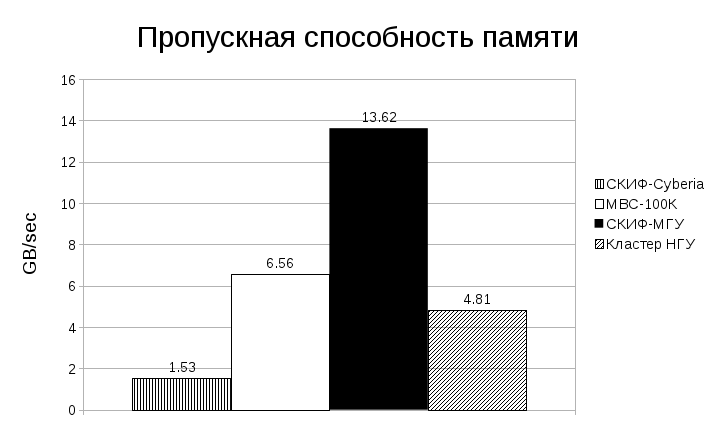
\includegraphics[height=7cm,keepaspectratio]{images/data_proc_throughput_GBsec.png}
	\end{center}
	\caption{Пропускная способность памяти на этапе расчета движения модельных частиц на некоторых кластерах. Количество модельных частиц: 2.5 млн. на каждое процессорное ядро. Основные параметры ВС, использованных в эксперименте, показаны в таблице \ref{top50_2010}.}
	\label{PIC_RAM}
\end{figure}
Следует отметить, что вопрос о сравнении чисел на рис. \ref{PIC_RAM} с заявленной максимальной пропускной способностью 
является второстепенным, тем не менее, сравнение показано в таблице \ref{PIC_vs_PROC_RAM}. Основной вопрос в данном случае - это измерение пропускной способности памяти,  фактически доступной для расчетного приложения.

\begin{table}[ht]
\caption{Сравнение пропускной способности памяти, измеренной с помощью теста на основе метода частиц с характеристиками процессора.}
\label{PIC_vs_PROC_RAM}
\begin{tabular}{|c|c|c|c|}
	\hline
             &            & \multicolumn{2}{|c|}{Пропускная способность памяти, GB/sec} \\ \cline{3-4}  	
Название ВС  & Процессор  & Данные теста MANAS & Максимум \\ \hline
МВС-100К     & Xeon E5450 &     6.02           & 21       \\ \hline 
СКИФ-МГУ     & Xeon E5472 &     12.47          & 21       \\ \hline     
СКИФ-Cyberia & Xeon 5150  &     1.45           & 10.6     \\ \hline
Кластер НГУ  & Xeon 5355  &     4.47           & 21       \\ \hline
\end{tabular}	
\end{table}

\section{Расчет производительности процессорных элементов}
\label{calc_PE}
В \textit{первом разделе} описана методика измерения производительности процессорных элементов.
Для того, чтобы отделить время счета от времени обращения к оперативной памяти было рассмотрено время работы процедуры,
реализующей одномерное преобразование Фурье, которая является частью физической диагностики, используемой в при моделировании динамики плазмы. Измереннное время с учетом известного размера данных и и количества операций в БПФ , переводится во флопсы. Сравнительная производительность процессорных элементов некоторых из рассмотренных в диссертационной работе ВС выглядит как показано на рисунке  \ref{procs_flops}:

\begin{figure}[htb]
	\begin{center}
		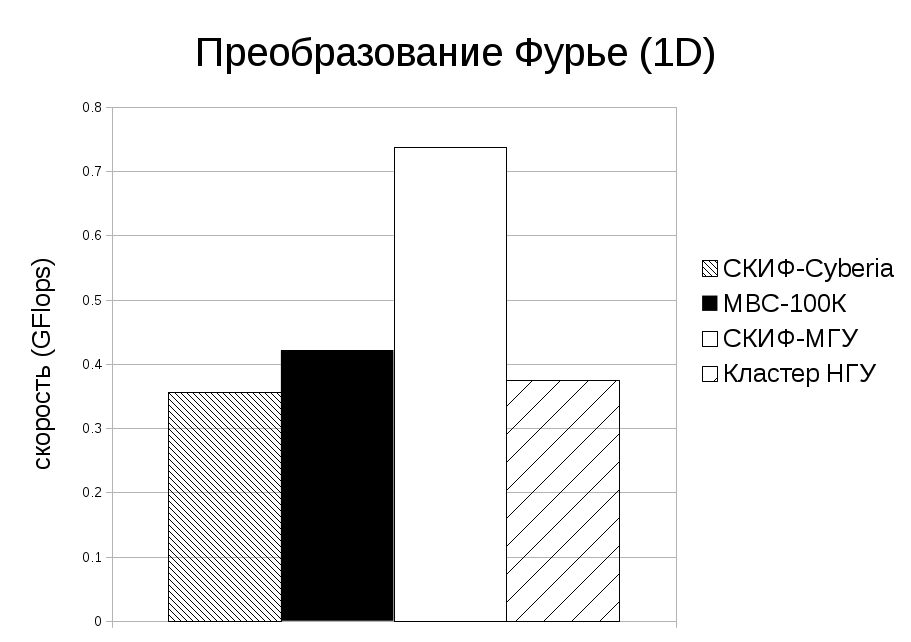
\includegraphics[height=7cm,keepaspectratio]{images/processor_FLOPS.png}
	\end{center}
	\caption{Производительность процессоров Intel Xeon, измеренная в ходе выполнения одномерного преобразования Фурье на некоторых кластерах. Размерность преобразования $N=64$. Измерения выполнены в 2010 г.}
	\label{procs_flops}
\end{figure} 


\section{Расчет производительности процессорных элементов на основе движения модельных частиц}
\label{calc_PE}
В \textit{первом разделе} описана методика измерения производительности процессорных элементов.
Для того, чтобы отделить время счета от времени обращения к оперативной памяти было рассмотрено время работы процедуры,
реализующей одномерное преобразование Фурье, которая является частью физической диагностики, используемой в при моделировании динамики плазмы. Измереннное время с учетом известного размера данных и и количества операций в БПФ , переводится во флопсы. Сравнительная производительность процессорных элементов некоторых из рассмотренных в диссертационной работе ВС выглядит как показано на рисунке  \ref{procs_flops_pic}:

\begin{figure}[htb]
	\begin{center}
		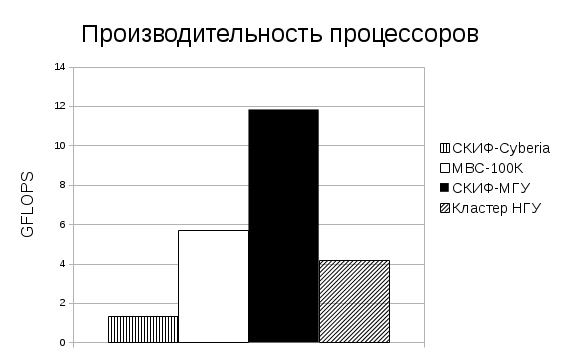
\includegraphics[height=10cm,keepaspectratio]{images/processor_FLOPS_PIC.png}
	\end{center}
	\caption{Производительность процессоров Intel Xeon, измеренная на основе времени вычисления движения модельных частиц. Измерения выполнены в 2010 г.}
	\label{procs_flops_pic}
\end{figure} 

Расчет количества операций с плавающей точкой в секунду (FLOPS) при расчете движения модельных частиц $N_{PIC,FLOPS}$ производился следующим образом:
$$
N_{PIC,FLOPS} = \frac{F_P\times N_P \times P_{core}}{\Delta t}
$$
здесь:
\begin{itemize}
	\item $F_P$ - количество операций на одну модельную частицу, $F_P = 500$;
	\item $N_P$ - количество модельных частиц на одно процессорное ядро (в рассмотренном случае $2.5\times 10^6$);  
	\item $P_{core}$ - количество ядер процессора;
	\item $\Delta t$  - длительность временного шага, сек.
\end{itemize}	

\begin{table}[ht]
	\caption{Производительность процессоров Intel Xeon, измеренная на основе времени вычисления движения модельных частиц.}
	\label{PIC_vs_PROC_RAM}
	\begin{tabular}{|c|c|c|c|c|c|}
		\hline
		&            &            &             &       \multicolumn{2}{|c|}{Производительность, GFLOPS} \\ \cline{5-6}  	
		Название ВС  & Процессор  &  $\Delta t$ &$P_{core}$ & Данные теста  &  \\
		             &            &             &           & PIC-MANAS     & LU-разложение \\ \hline
		МВС-100К     & Xeon E5450 &  0.878      & 4     & 5.69           & 4.6     \\ \hline 
		СКИФ-МГУ     & Xeon E5472 &  0.423      & 4     & 11.83          & 2.37       \\ \hline     
		СКИФ-Cyberia & Xeon 5150  &  1.882      & 2     &  1.33          & 4.65    \\ \hline
		Кластер НГУ  & Xeon 5355  &  1.196      & 4     & 4.18           & 1.82       \\ \hline
	\end{tabular}	
\end{table}






\subsubsection{Расчет производительности коммуникационной сети}
\label{perfCommNet}
В \textit{третьем разделе} приведена методика измерения быстродействия коммуникационной сети на основе анализа времени работы MPI-процедур, осуществляющих обмен граничными значениями между отдельными подобластями при решении уравнений Максвелла и при пересылке модельных частиц. В силу того, что при этом используются различные виды коммуникационных функций  - как блокирующие, так и не блокирующие, как парные, так и коллективные, при использовании эйлерово-лагранжевой декомпозиции - это позволяет набрать в течение одного расчета большую базу данных для получения знаний о структуре коммуникационной сети, времени прохождения сообщений в зависимости от размера, системных таймаутах и пр. 

В данном случае показан более простой и более ограниченный тест, полученный на основе измерения времени пересылки модельных частиц, перелетающих из одной подобласти в другую (эйлерова или эйлерово-лагранжева декопозиция). Эмпирические факты таковы, что из подобласти в подобласть перелетает около 5 \% имеющихся частиц. В принципе, может перемещается и больше, если выполняется моделирование плазменной турбулентности, приводящей к возникновению больших потоков вещества, в таком случае просто измеряется количество перемещенных частиц. Но это уже другая физическая постановка задачи.

Далее, количество частиц в данном расчете составляет 2.5 млн. на одно процессорное ядро, каждая частица занимает 48 байт (три координаты и три компоненты имульса в двойной точности), всего 114.4 Мб на ядро. Если перемещается около 5\%, то это 5.72 Мб в течение каждого временного шага в методе частиц в ячейках. В таблице \ref{tab_net_gb_sec} показано время работы процедуры, выполняющей передачу модельных частиц, и вычисленная на основе этого производительность коммуникационной сети.


Вычисление производительности коммуникационной сети $U_{PIC,GB/sec}$ на основе данных о пересылке модельных частиц между  производится по следующией формуле:
$$
U_{PIC,GB/sec} = \frac{U_P\times \nu N_P \times P_{core}}{T_{S,PIC}}
$$
здесь:
\begin{itemize}
	\item $U_P$ - количество байт на одну модельную частицу, $U_P = 48$;
	\item $N_P$ - количество модельных частиц на одно процессорное ядро (в рассмотренном случае $2.5\times 10^6$);  
	\item $P_{core}$ - количество ядер процессора;
	\item $\nu$ - доля пересылаемых частиц (напомним, что обычно $\nu \approx 0.05$);
	\item $T_{S,PIC}$  - время пересылки частиц, сек.
\end{itemize}	



\begin{figure}[htb]
	\begin{center}
		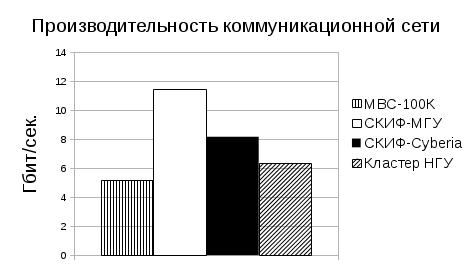
\includegraphics[height=10cm,keepaspectratio]{images/PIC_RAM_Gb_sec.png}
	\end{center}
	\caption{Производительность коммуникационной сети, измеренная на основе скорости пересылки модельных частиц. Измерения выполнены в 2010 г.}
	\label{plot_net_gb_sec}
\end{figure} 

Измеренные данные необходимо сравнивать с заявленными показателями производительности оборудования. Так, производительность сети Infiniband 4x составляла до 32.96 Гбит/с на 2010 г.,  а для Gigabit Ethernet - 10 Гбит/с  

\begin{table}[ht]
	\caption{Сравнение производительности коммуникационной сети, измеренной с помощью теста на основе метода частиц (используются операции MPI\_Send/MPI\_Recv) с характеристиками оборудования.}
	\label{tab_net_gb_sec}
	\begin{tabular}{|c|c|c|c|c|}
		\hline
		             &                     &        &    \multicolumn{2}{|c|}{Производительность,} \\ 
		             &                     & Время            &    \multicolumn{2}{|c|}{Гбит/с} \\ \cline{4-5}              
		Название ВС  & Сеть                & пересылки   & Данные теста       & Максимум  \\
		             &                     & частиц, сек.&   PIC-MANAS        &           \\  \hline
		МВС-100К     &  Infiniband 4x DDR/ &  0.011           &     5.2           & 32       \\ 
		             &  2xGigabit Ethernet/&             &                    &          \\
		             &                     &             &                    &          \\ \hline  
		СКИФ-МГУ     & InfiniBand/         &  0.005           &     11.44          & 32       \\   
		             &  Gigabit Ethernet/  &              &                    &          \\
		             &  СКИФ-ServNet       &              &                    &          \\   
		             &   + IPMI            &             &                     &          \\ \hline  
		СКИФ-Cyberia &  QLogic InfiniPath/ &  0.007           &      8.17              & 10    \\ 
		             &  Gigabit Ethernet/  &             &                    &          \\
		             &  СКИФ-ServNet       &             &                    &          \\ \hline
		Кластер НГУ  & Infiniband 4x DDR/  &  0.009        &     6.35           & 32       \\ 
		             &   Gigabit Ethernet/ &           &                    &          \\
		             &   Gigabit Ethernet  &           &                    &          \\ \hline
	\end{tabular}	
\end{table}

\clearpage



%		На  рисунке приведено скорость обмена данными между процессами (график из статьи в Мб/сек) 
%		\textbf{перерисовать графики МВС-100К и Ломоносов в общей части}	
%		
%		
%		Сравнение графиков ускорения, полученных на МВС-100К, Ломоносов НГУ и пр.

\section{Формула для комплексной оценки ВС}
\label{complex_evaluation}
В \textit{четвертом разделе} приведено обоснование формулы, на основании которой выносится оценка ВС по материалам проведенных тестов. При этом важно отметить, что оценка является не сравнительной - относительно других ВС, а абсолютной - с точки зрения математического моделирования. 

В частности, для того, чтобы параллельная ВС могла быть признана адаптированной к задачам математического моделирования, она должна соответвовать следующим требованиям:
\begin{enumerate}
	\item Относительно высокая производительность коммуникационной сети, позволяющая пересылать все необходимые для расчета данные, не задерживая вычислений
	\item Очень высокая пропускная способность дисковой подсистемы, обеспечивающая сохранение больших объемов данных, полученных в результате счета  	
\end{enumerate}

Важно отметить, что названы относительные показатели, обеспечивающие возможность пересылать и сохранять данные, без ущерба для скорости вычислений. Именно это и означает  комплексную пригодность ВС к решению задач математического моделирования, т.е. результаты счета сохраняются на диск с той же скоростью, с которой пересылаются данные между узлами данной ВС, и более того, эта скорость не намного меньше скорости вычислений.

Для того, чтобы все три упомянутые величины могли быть использованы в одной формуле, необходимо 
\begin{itemize}
	\item привести эти величины к одной размерности (скорость вычислений выражается во флопсах, скорость обмена данными - в гигабайтах в секунду)
	\item представить обобщенные коэффициенты, позволяющие сравнивать объем данных, сохраняемых на диск и объем данных, пересылаемых по коммуникационной сети ВС  
\end{itemize}


Для решения обоих этих задач использованы усредненные данные расчетов по методу частиц в ячейках на различных ВС. Данный метод может быть использован как оценка снизу, т.е. пригодность некоторой ВС для проведения расчетов по методу частиц в ячейках может трактоваться как возможность проведения расчетов по широкому спектру вычислительных методов, причем, как правило, с большей эффективностью.

Итак, коэффициент перевода из флопсов в байты в секунду для расчетов с частицами равен
$k_{f2b} = 500/576$ = 0.86   
и коээфициент для перевода объема данных, сохраняемых на диск к объему данных, пересылаемых по коммуникационной сети, аналогично, для частиц равен (усредненно):
$k_{MPI} = 0.05$ 
Это объясняется тем, что в среднем не более 5\% частиц пересылается между подобластями.
В итоге формула оценки $\xi$ имеет вид:
$$
\xi = \frac{W_{MPI}} {k_{f2b} W_{PIC}}, 
$$
при условии, что $W_{disc} \approx W_{MPI}$,
здесь $W_{disc}$ - скорость работы дисковой подсистемы (байт/сек), $W_{MPI}$
- скорость пересылки данных по сети - (байт/сек) и $W_{PIC}$ - скорость расчета по частицам (во флопсах).	

           % Глава 3
\chapter{Анализ масштабируемости, параллельной эффективности и ускорения параллельной ВС}
			%	ОБЩЕЕ ПРАВИЛО ДЛЯ ВТОРОЙ ГЛАВЫ: НЕ ПЛАНРИРОВАТЬ ЧТО_ТО НОВОЕ И ОЧЕНЬ ХОРОШЕЕ ЧЕГТО НЕТ, А ПОДКРЕЛЯТЬ И УИСИЛВАТЬ ТО, ЧТО РЕАЛЬНО ЕСТЬ.
			%	ЕСЛИ У НАС СЛАСБОСТЬ В ОБЛАСТИ АНАЛИЗА КОММ СТРУКТУРЫ - НУ И ЛАДНО, И ПУСТЬ ОНА БУДЕТ. ГОВОРИТЬ БОЛЬШЕ О МАСШТАБИРУЕМОСТИ. А КОРММ СТРУКТУРУ АНАЛИЗИРПОВАТЬ ЧЕРЕЗ ПЕРЕСЫЛКИ ЧАСТИЦ
			%	НАША ИДЕЯ не ПОДМЕНЯТЬ СОБОЙ ДИАГНОСТИКУ АРХИТЕКТУРЫ, а мерять И ОПРЕДЕЛЯТЬ ВСЕ ЧЕРЕЗ ИЗМЕРЕНИЯ ВРЕМЕН ПО PIC
				В четвертой главе предложена методика интегральной оценки тестируемой ВС с помощью измерения масштабируемости с расчетах по методу частиц в ячейках и определения на основе измерений возрастания потока данных в коммуникационной сети ВС.
%				На основе данных о пересылке модельных частиц измерена производительность коммуникационной сети ВС, при этом важно отметить преимущества использованного метода измерений: пересылка данных имеет высокую степень нерегулярности, а также большой объем, что означает проведение тестирования на большой нагрузке, и возможность широкого применения полученных таким образом данных.
%				Также предложена и апробирована методика определения фактически соседних (с точки зрения MPI) узлов ВС.  
							
			\section{Определение понятий эффективности, масштабируемости и ускорения}
			%\textbf{Степаненко, книжка"высокопроизводительные вычисления", учебник Воеводина}
			
			Выписано определение эффективности параллельной реализации программ, сильной и слабой масштабируемости, ускорения при распараллеливании.
			
			В частности, ускорение параллельного алгоритма для $N$ процессоров, определяется как:
			$$
			S_N = \frac{T_1(n)}{T_N(n)}
			$$  
			здесь $T_1$ - время исполнения алгоритма на одном процессоре, $T_N$ - на $N$ процессорах, величина $n$ характеризует вычислительную сложность решаемой задачи, для определения ускорения существенно, что задачи, решаемые на 1 и на $N$ процессорах имеют одинаковую сложность.
			Далее, эффективность распараллеливания вычисляется как
			$$
			\eta_N = \frac{1}{N}\frac{T_1(n)}{T_N(n)}
			$$  
			эта величина иногда называется эффективностью в сильном смысле (англ. strong efficiency). Кроме того, часто используется эффективность в слабом смысле (англ. weak efficiency):
			\begin{equation}
			\label{weak_eff}
			\eta^{weak}_N = \frac{T_1(1)}{T_N(N)}
			\end{equation}
			здесь, в отличие от определения ускорения, задачи, решаемые на одном и на $N$ процессорах, имеют различную сложность, т.е. при увеличении количества процессоров в $N$ раз сложность задачи такжэе увеличивается в $N$ раз, и таким образом определяемая эффективность будет 100 \% в том случае, если время вычислений не возрастает при увеличении сложности задачи пропорциональном увеличению количества процессоров.   
			
			Приведены различные используемые варианты этих определений, перечислены факторы, влияющие на  значения этих величин для конкретной ВС, а именно скорость обмена данными и структура коммуникационной сети ВВС, алгоритмы реализации MPI-процедур, в особенности коллективных, настройки коммуникационной системы (таймауты, размер системных буферов, и др.).
			%\textbf{написать формулы} 
			%\textbf{привести формулы из статьи в СибЖВМ}
			Для последующего анализа измереннного времени работы метода частиц в ячейках на параллельной ВС, и для прояснения зависимости этого времени от параметров расчета можно привести следующую схематическую формулу для длительности одного временного шага, аналогично статье (Вшивков В.А. и др., СибЖВМ, 2003):
			
			\begin{equation}
			\label{PIC-timestep}
			T=T_{F} \left ( \frac{N_x N_y N_z }{P_E}\right )+ T_{F,S}\left (N_y N_z\right ) + T_P\left(\frac{N_p}{P_E\times P_L}\right) +T_{P,S}\left (\frac{N_p*T_p}{P_E\times P_L}\right)
		\end{equation}
			 
		здесь $T_{F}$ - время вычисления электромагнитного поля, $N_x, N_y, N_z$ - размер расчетной сетки соответственно, по координатам $X$ $Y$ и $Z$, $P_E$ - количество процессоров для эйлеровой декомпозиции, т.е. для разделения расчетной области на подобласти, $T_{F,S}$ - время, затрачиваемое на персылку граничных значений полей и токов между подобластями, которое зависит только от $N_y$ и $N_z$ в силу того что на данный момент используется одномерная декомпозиция,  $T_P$ - время расчета движения частиц, $P_L$ - количество процессов (или потоков) для лагранжевой декомпозиции, т.е. для дополнительного разделения частиц подобласти на группы, вычисляемые на отдельных ядрах.
		
		

		
		
		\section{Анализ масштабируемости как интегральной характеристики ВС.}
		
		Во втором разделе приведены фактически измеренные на различных высокопроизводительных ВС графики масштабируемости и параллельной эффективности и на основе этих данных проведен анлиз коммуникационной сети данных ВС, в частности, для МВС-100К, рис. \ref{eff2}. 
		
		\begin{figure}[h]
			\begin{center}
				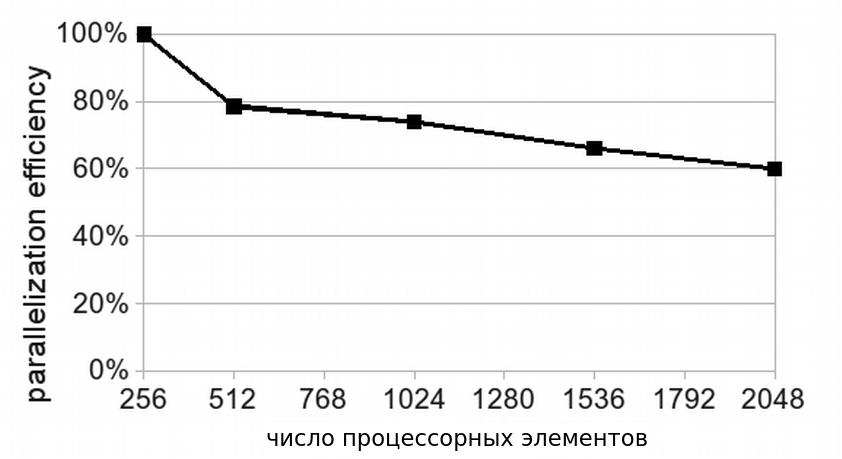
\includegraphics[height=5cm,keepaspectratio]{images/eff_weak_JSCC.png}
				\caption{
					Эффективность распараллеливания в слабом смысле, для МВС-100К, МСЦ РАН.
				}
				\label{eff2}
			\end{center} 
		\end{figure}
		
		Возможность проведения анализа коммуникационной сети с помщью расчетов по методу частиц в ячейках основана на известной информации о количестве пересылаемых данных и о виртуальной топологии, используемой в программе.
		
		Размер данных, перемещаемых между двумя соседними MPI-процессами равен $144 \times N_y N_z  $ байт. При этом в идеальном случае, когда соседние MPI-процессы находятся на соседних узлах, коммуникации происходят только между соседними узлами, и поток данных в системе в целом не возрастает с ростом количества используемых в расчете узлов.
		
		В частности, в расчете показанном на рис. \ref{eff2} использована эйлерова декомпозиция. Это означает, что используются только парные пересылки MPI, коллективные пересылки не используются, и поток данных через коммуникационную систему ВС в целом возрастать не должен. Если, тем не менее, он возрастает, что видно на рис. \ref{eff2} в виде снижения эффективности распараллеливания, то это может (при отсутствии коллективных операций), означать, что соседние с точки зрения MPI процессы находятся на физически удаленных друг от друга узлах параллельной ВС.
		
		Обозначая $k_{||}$ зависимость коэффициента при времени пересылок граничных условий от количества процессоров в формуле \ref{PIC-timestep}, так что 
		\begin{equation}
		T_{F,S} = k_{||} (P_E) \frac{N_y N_z}{P_E}
		\end{equation} 
		и подставляя формулу \ref{PIC-timestep} d \ref{weak_eff}, рассматривая только лишь время расчета и пересылок электромагнитного поля, можно получить 
		\begin{equation}
		k_{||} (P_E) = \frac{1}{\eta^{weak}(P_E)} - 1
		\end{equation}	  
		Таким образом величина $k_{||} (P_E)$  - \textbf{степень нелинейности} коммуникационной структуры параллельной ВС. Фактически она представляет собой отклонение от линейной функции для зависимости времени пересылок от количества процессоров. Он показывает предел возрастания потока данных через коммуникационную структуру ВС при увеличении количества процессоров, используемых в расчете. Эта величина характеризует, в какой степени при передаче информации между соседними процессами в MPI используются узлы параллельной ВС, не являющиеся ближайшими соседями. В силу того, что на значение эффективности оказывает влияние не только свойства оборудования, но и особенност реализации MPI, возникает необходимость разделить эти факторы. Это достигается с помощью привязки процессорв к узлам. 
		
		В итоге, такимобразом определенная  величина $k_{||} $ может быть использована как характеристика параллельной ВС, показывающая реально достижимую с помощью данной ВС эффективность и масштабируемость   
		
		\subsection{Измерение продолжительности параллельных коммуникаций и анализ характеристик и топологии коммуникационного оборудования}
		Здесь описано решение задачи об определении соседства процессов по реальным узлам. Это исключительно важно для производительности реальных задач, чтобы виртуально близкие (т.е. по номеру MPI-процесса) процессы исполнялись бы на соседних узлах многопроцессорной ВС. Для этого проводится обмен сообщениями между узлами, выделенными 
		для исполнения программы по топологии полного графа, и проводится анализ времени прохождения сообщений, рис. \ref{poly_all2all}.  
		
		Следует отметить, что такого этапа, с обменом сообщениями между всеми процессами в рамках метода частиц нет, поэтому, такой анализ проводится предварительно, перед запуском основной части программы.

		
		\begin{figure}[htb]
			\begin{center}
				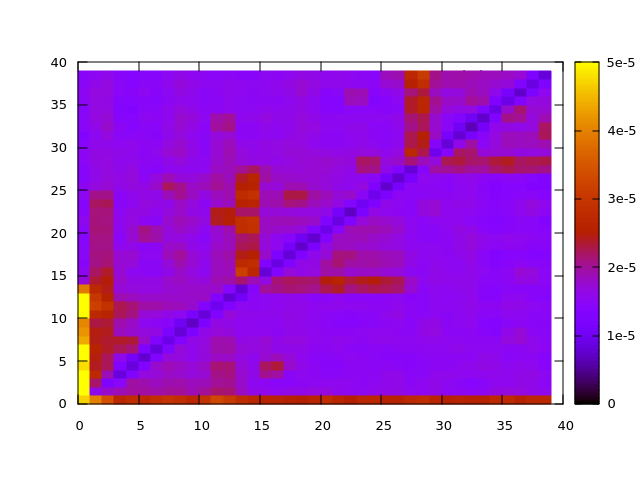
\includegraphics[height=7cm,keepaspectratio]{images/polytech_all_to_all.png}
			\end{center}
			\caption{Время пересылок для 40 MPI-процессов, расположенных на 10 узлах по 4 процесса, кластер «Политехник», СПбПУ. По осям X и Y отложены номера процессов, цветовая шкала показывает время пересылок в секундах.}
			\label{poly_all2all}
		\end{figure} 
		Узлы с минимальным временем считаются близкими, т.е. выясняется фактическая топология ВС. Это сопоставляется с известной информацией о размещении процессов по узлам.	Для повышения производительности приложения в дальнейшем целесообразно передвинуть соседние процессы на те узлы, где по факту меньше задержка по коммуникациям.
		
		%	\textbf{картинку из стьатьи все-со-всеми, (с Политеха)}. 
		%	1.измерение всех видов MPI-коммуникаций, сравнение одного с другим (Send, Isend, Bsend) - и увязатиь это с алгоритмом
		%	2. варьирование размера сообщений и пр. параметров
		
	%	\textbf{материал статьи НГУ ИТ  с более аакуратным анализом}
        \section{Оценки параллельной масштабируемости на основе измерений времени прохождения сообщений}
        
        С этим связан основные вопросы настоящей статьи: 
        что, если группа процессов, которые должны осуществлять коллективные пересылки, окажется размещенной на узлах суперЭВМ, расположенных физически далеко друг от друга, так что время выполнения этих пересылок будет велико?
        Как можно избежать такой ситуации, как объединять в группы для коллективных пересылок близко расположенные процессы, при том что MPI (или система очередей) размещает процессы на узлах фактически случайным образом? 
        Как можно заранее оценить трудоемкость коммуникационных операций и выработать оптимальную схему размещения процессов? 
        На основании чего можно принимать решение о перемещении процессов с одного узла на другой, или о перенумерации процессов? 
        В некоторых случаях эти вопросы решаются специально созданными внешними инструментами [10, 11], но для рассматриваемой в данной работе программы целесообразным является иметь собственные средства для решения проблемы неудачного размещения на узлах.
        Для того, чтобы частично ответить на эти вопросы, были проведены вычислительные эксперименты на нескольких суперЭВМ с измерением производительности различных коммуникационных операций, построены оценки трудоемкости этих операций и предложен метод выделения групп близко расположенных процессов. Создать правильное представление о реальной длительности коммуникаций между процессами в программе важно также для того, чтобы решить вопрос о целесообразности использования динамической балансировки и для выбора конкретного ее варианта [12-14], и о применении форм-факторов высокого порядка [15-16] в методе частиц в ячейках [17,18, 19]. 
        
        Краткое описание вычислительных экспериментов
        
        Задавались следующие основные параметры и числовые характеристики тестовых расчетов:
        
        NX, NY, NZ,  - размер сетки по каждому из измерений (NX, NY – от 100 до 500, NZ = 20)
        PALL  - общее количество процессорных ядер (до 1000)
        PSUB  - число подобластей (до 20)
        
        Измерялись кроме физических величин, следующие времена (с помощью Intel Trace Analyzer &Collector, https://software.intel.com/en-us/intel-trace-analyzer):
        
        T – длительность тестового расчета (50 временных шагов), сек.
        t  - длительность временного шага, сек.
        TMPI_All - длительность операции MPI_Allreduce (суммирование токов по всей области), сек.
        TMPI_Send - длительность операции MPI_Sendrecv (обмен граничными значениями), сек.
        
        \textbf{посмотреть отчеты РНФ - графики и описания}
        
        Расчеты проводились на следующих суперЭВМ:
        Кластер НГУ. Из различных имеющихся типов узлов использовались только узлы  HP BL2x220c G6, каждый из которых содержит две материнские платы, на каждой из которых: два 4-ядерных процессора Intel Xeon E5540 с тактовой частотой 2530 МГц и 16 ГБ ОЗУ
        Кластер СПбПУ «Политехник». Использовались узлы с двумя 28-ядерными процессорами  Intel®Xeon® E5-2600 v3
        Кластер «Ломоносов» в НИВЦ МГУ. Использовались узлы основного раздела, содержащие 2 4-ядерных процессора Intel Xeon  X5570 
        Физические параметры проводимых в данной работе расчетов соответствуют кинетическому режиму развития двухпотоковой неустойчивости, рассмотренному в [20].
        Верификация формул для оценки времени работы коммуникационных процедур
        Для оценки времени работы коммуникационных процедур, в первую очередь MPI_Allreduce и MPI_Send/MPI_Recv с целью выработки оптимальной схемы размещения процессов исходя из реально выделенных (системой очередей) вычислительных ресурсов, можно использовать следующие простые формулы:
        
        
        ,
        где T- время пересылки данных, N – количество процессов (ядер), a и b – константы, зависящие от архитектуры суперЭВМ, количества пересылаемых данных, реализации MPI и др. На рисунках 2-4 и 5-7 показаны результаты аппроксимации реальных данных о продолжительности пересылок, полученных в ходе вычислительных экспериментов, описанных в предыдущем разделе. На рисунках приведены аппроксимирующие формулы, и указано значение среднеквадратической ошибки, позволяющее определить наилучший тип аппроксимации. На рисунках 2-4 и 5-7 показаны данные, измеренные на всех кластерах, на которых проводились расчеты, т.е. особенности архитектуры здесь не учитываются.
        Каждая точка на рисунках 2-4 и 5-7 представляет собой отдельный расчет. Все расчеты проведены на разных архитектурах, количество ядер соответствует количеству MPI-процессов. Возможно, что запуски на 50, 150 ядер аннулируют все догадки и предположения, а может наоборот вычертят кривую, т.е. полученные результаты имеют предварительный характер.
        
        Рис.2. Продолжительность операции MPI_Allreduce. Линейная аппроксимация.
        
        Рис.3. Продолжительность операции MPI_Allreduce. Степенная аппроксимация.
        
        Рис.4. Продолжительность операции MPI_Allreduce. Экспоненциальная аппроксимация.
        Из рисунков 2-4 видно, что наименьшее значение среднеквадратической ошибки достигнуто при степенной аппроксимации:
        T = 0.0056*N0.214
        Далее рассмотрим парные пересылки. Зависимость от числа ядер в данном случае возникает потому, что в таких пересылках задействованы все ядра, между которыми разделена область: MPI-процесс, работающий на каждом ядре пересылает данные обоим своим соседям. Фактически речь идет о длительности эйлерова этапа параллельного алгоритма.
        
        Рис.5. Продолжительность операции MPI_Send. Линейная аппроксимация.
        
        Рис.6. Продолжительность операции MPI_Send. Степенная аппроксимация. 
        
        Рис.7. Продолжительность операции MPI_Send. Экспоненциальная аппроксимация. 
        В этом случае наименьшая ошибка оказалась достигнута при экспоненциальной аппроксимации:
        T = 0.0077*exp(-0.00562*N)
        
        
        
        Полученные формулы не является зависимостями, работающими всегда, на любых суперЭВМ, любых реализациях MPI и т.д. Их назначение в том, чтобы в ходе реального крупномасштабного расчета, без повторных запусков, не прерывая счет, ответить на вопрос, что будет, если увеличить количество процессоров (ядер), вовлеченных в коллективные взаимодействия. Т.е. в данном случае предполагается динамическое дозапускание MPI процессов, допустимое стандартом MPI2.
        Например, программа, использующая 40 MPI-процессов  получила для счета 40 ядер. Эти ядра можно по-разному распределить между эйлерой и лагранжевой декомпозицией области: можно поделить область на 10 частей, и затем распределить все частицы каждой подобласти между  4 MPI-процессами, а можно наоборот. Даже для 40 процессов есть несколько вариантов, в то время как речь идет о расчетах на нескольких тысячах ядер, где невозможно будет просто перебрать все варианты и выбрать оптимальный.
        Для того, чтобы сделать правильный выбор, предлагается после выделения узлов для счета провести несколько тестовых запусков коллективных операций, построить для данного конкретного расчета аппроксимацию, подобную полученной выше, и на ее основе принимать решение.
        
        
        
        
        
        
        
        \section{Определение коммуникационной структуры ВС}
        
        MPI предоставляет пользователю возможность создания собственных виртуальных топологий, в том числе декартовых (двумерных, трехмерных  и пр.). При этом в соответствии со стандартом процессы, расположенные на физически близких узлах, должны иметь близкие номера в рамках топологии, однако все зависит от конкретной реализации MPI.  
        Для решения этого вопроса в описанной программе реализован специальный диагностический модуль, выполняющий пересылки типа «точка-точка» (MPI_Send/MPI_Recv) между всеми процессами (all-to-all, «каждый с каждым»). При этом рассматривались разные варианты размещения процессов по узлам. В каждом случае измерялось время пересылки с помощью функции MPI_Wtime. На рисунках 8-13 показано время пересылок во всех парах взаимодействующих процессов.
        
        Рис.8. Время пересылок для 4 MPI-процессов, расположенных на двух узлах попарно, кластер НГУ.
        На рисунке 2 видно, что время пересылок внутри узла (0-й процесс и 1-й, или 3-й и 4-й) меньше, чем время пересылок между узлами. Для того, чтобы аналогичным образом рассмотреть более сложные конфигурации, необходимо перейти от трехмерной столбчатой диаграммы к двумерным картам плотности, например, рис.9. 
        
        Рис.9. Время пересылок для 16 MPI-процессов, расположенных на двух узлах по 8 процессов, кластер НГУ. По осям X и Y отложены номера процессов, цветовая шкала показывает время пересылок в секундах.
        Рисунок 9 естественным образом разбивается на 4 зоны, соответствующих размещению процессов по узлам, несмотря на то, что принципиальной разницы по времени пересылок между узлами и внутри узлов в данном случае нет.
        
        Рис.10. Время пересылок для 40 MPI-процессов, расположенных на 10 узлах по 4 процесса, кластер НГУ. По осям X и Y отложены номера процессов, цветовая шкала показывает время пересылок в секундах.
        На рисунке 10 не удается зрительно выделить 10 зон, соответствующих 10 узлам, на которые проводился расчет. Тем не менее видно, что участки с наименьшими временами пересылок расположены вдоль диагонали матрицы, как и на предыдущих рисунках.
        Следует отметить, что такая задача безусловно и не должна решаться «на глаз», в дальнейшем планируется применить здесь известные методы выделения сообществ в полном графе. Задача данной работы только в том, чтобы проверить обмен сообщениями у попарно между всеми процессами как метод тестирования архитектуры кластера: позволяет ли он выявлять отличие между близко и далеко расположенными процессами. Для этого обратимся к суперЭВМ существенно отличной архитектуры, а именно кластеру «Политехник» в СПбПУ.
        
        Рис.11. Время пересылок для 40 MPI-процессов, расположенных на 10 узлах по 4 процесса, кластер «Политехник», СПбПУ. По осям X и Y отложены номера процессов, цветовая шкала показывает время пересылок в секундах.
        В первую очередь важно отметить, что на рисунке 11 все времена на порядок меньше, чем на рис. 10, показывающем ту же конфигурацию для кластера НГУ. Далее, на рис.11 видны прямоугольные участки с большим временем пересылок (красного цвета), шириной в 4 процесса, расположенные как горизонтально, так и вертикально. Это говорит о том, что возможна ситуация, когда близко по номеру расположенные процессы будут иметь большее время обмена сообщениями по сравнению с более удаленными (в данном случае 13-15 процессы при обмене с  16-20 процессами). 
        
        Рис.12. Время пересылок для 40 MPI-процессов, расположенных на 4 узлах по 10 процессов, кластер «Политехник», СПбПУ. По осям X и Y отложены номера процессов, цветовая шкала показывает время пересылок в секундах.
        На рис. 12 показан расчет также с использованием 40 процессов, но размещенных на 4 узлах. Видно, что красные зоны (с большим временем пересылок) имеют больший размер и преимущественно локализованы в левой верхней и правой нижней четвертях квадрата, что соответствует обмену сообщениями между процессами, расположенными на разных узлах.
        
        Рис.13. Время пересылок для 100 MPI-процессов, расположенных на 10 узлах по 10 процессов, кластер «Политехник», СПбПУ. По осям X и Y отложены номера процессов, цветовая шкала показывает время пересылок в секундах.
        На рисунке 13 видны группы размером 5 процессов, время обмена между которыми заметно меньше, чем со всеми остальными. Это также коррелирует с их размещением по узлам.
        По итогам анализа рисунков 2-7 можно сделать вывод, что использованный метод анализа архитектуры суперЭВМ позволяет обнаружить группы близко расположенных процессов.
        
        
        
        
        
        
        
        \textbf{Заключение}
        
        
        В заключение можно дать следующие рекомендации для использования конкретного варианта декомпозиции в зависимости от реально доступной коммуникационной структуры суперЭВМ:
        Использовать для лагранжевой декомпозиции только близко (внутри одного узла, или на соседних узлах) расположенные процессы, или в рамках узла использовать OpenMP.
        Не назначать соседние подобласти в рамках эйлеровой декомпозиции на далеко разнесенные узлы
        Приоритетной считать эйлерову декомпозицию в том случае, если память узла позволяет разместить соответствующий фрагмент данных
        
        
		\subsubsection{Измерение производительности коммуникационной сети на основе данных о пересылке модельных частиц}
		В \textit{четвертом разделе} приведены результаты измерения скорости пересылок модельных частиц в методе частиц в ячейках и проведенный на основе этого сравнительный анализ скорости работы коммуникационной сети ВС.
		
		На нескольких параллельных ВС были измерены времена, затраченные на пересылку модельных частиц между соседними узлами. Из статитики расчетов по методу частиц в ячейках известно, что пересылается, как правило, не более 5\% модельных частиц. В рассматриваемых расчетах размер сетки $512\times 64 \times 64$ узла  при 150 модельных частицах в ячейке, т.е.  на каждом временном шаге в среднем пересылается 15.7 млн. модельных частиц, что при размере одной частицы в 48 байт означает 720 Мб на каждый временной шаг, что при известном времени пересылки позволяет вычислить скорость. Таким образом была экспериментально измерена величина $T_{P,S}$, входящая в формулу \ref{PIC-timestep}   
			
			\begin{figure}[htb]
				\begin{center}
					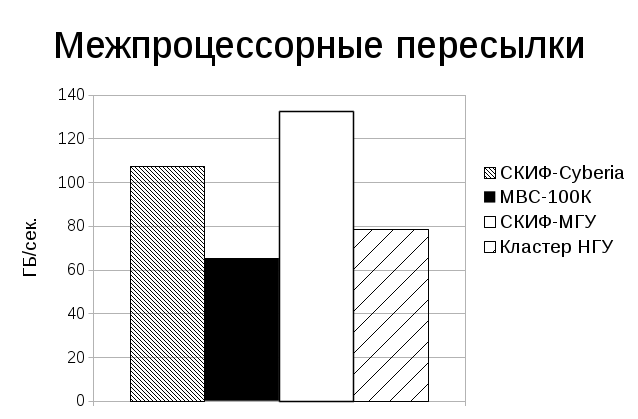
\includegraphics[height=7cm,keepaspectratio]{images/particle_send_GBsec.png}
				\end{center}
				\caption{Скорость пересылки данных на некоторых кластерах. Количество модельных частиц: 2.5 млн. на каждое процессорное ядро. Измерения выполнены в 2010 г.}
				\label{procs_flops}
			\end{figure}
			
			Измеренная таким образом скорость пересылки данных показывает фактический предел этой величины, реально достижимый для вычислительного приложения с использованием имеющегося оборудования и коммуникационного программного обеспечения. Это подтверждается следующими соображениями:
			\begin{itemize}
				\item Объем пересылаемых данных мал: в среднем 6 Мб на процесс
				\item Соседние MPI-процессы, как правило, расположены на близких узлах.
			\end{itemize}  	 
			
		%	\subsubsection{Экстраполяция результатов тестирования ускорения и эффективности распараллеливания}
			%%	формулы из статьи НГУ-ИТ'17, адаптированные и улучшенные, сравнение со Степаненко
			%%	выводы по большой системе на тех же принципах, совпадение с реальностью
			%%	
			%	В \textit{четвертом разделе} описана оригинальная методика экстраполяции результатов на системы большой размерности и ее сравнение с аналогиными работами.Проведено большое количество физических расчетов с использованием программы в трехмерной расчетной области, использующей двухступенчатую эйлерово-лагранжеву декомпозицию расчетной области.На основании тестовых расчетов на небольшом количестве процессорных ядер измереятся время коллективных и парных коммуникаций MPI и строится аппроксимацию времени пересылок для произвольного количества процессов.
			
			%	Основным вопросом является соответствие реально измеряемого времени выполнения коммуникационных операций для определенного количества процессоров, 
			%	 По результатам вырабатываются рекомендации по выбору оптимального сочетания эйлеровой и лагранжевой декомпозиции.
			%	\textbf{формулы}
			
			%	\subsection{Глава 3: Анализ производительности системы памяти}
			%	\subsubsection{Кэш-память}    
			%	Статьи PACO (кэш, списки и пр.), BOE (данны исполения на Sun Sparc Opteron)
			%	\subsubsection{Оперативная память}
			%	 PAVT10, Абрау7 PACO           % Глава 4
%\chapter{Анализ производительности узлов мультиархитектурной ВС} \label{chapt3}
Описаны методы, позволяющие определять скорость счета на ускорителях вычислений и скорость перемещения данных между ускорителем вычислений и хост-машиной, а также давать прогнозы о скорости счета нереализованных еще алгоритмов на тестируемой ВС.

Кроме того, предложена методика оценки качества узлов мультиархитектурной ВС на основе графических ( или других) ускорителей, при этом качество понимается как сбалнсированность средней оценочной скорости счета на ускорителе и скорости пермещения данных между ускорителем и хостом
\cite{MohographyTarkov,VestnikNNSU,VestnikNSUadapt,VychMethProgExa,SuperFrI,astroCoDesign,integrApproach}.

CUDA Cores
4992


\section{Анализ производительности узлов с графическими ускорителями} \label{sect3_1}

\begin{table}[ht]
	\begin{center}
		\caption{Основные параметры GPU, использованных в тестах}
		\begin{tabular}{|c|c|c|c|c|c|}
			\hline
			Название          &GeForce  & M2090  & K40m    & K80    & P100  \\ \hline
			                  & GTX 850M&        &         &        &
			Объем             &         &        &         &        &       \\
			глобальной памяти & 4 GB    & 5.3GB  & 11.5GB  & 16 GB  & 16 GB \\ \hline
			Количество        &         &        &         &        &       \\
			мультипроцессоров & 5       &  16    & 15      & 26     &  56   \\ \hline
			Количество        &         &        &         &        &       \\
			ядер CUDA         & 640     & 512    & 2880    &  4992  & 3584  \\ \hline
			Тактовая частота  &         &        &         &        &        \\
			GPU               & 902 MHz &1301 MHz& 745 MHz & 560 MHz&  1328 MHz \\ \hline
			Ширина            &         &        &         &        &         \\
			шины памяти       & 128-bit & 384-bit& 384-bit & 384-bit&  4096-bit\\ \hline
		\end{tabular}
		\label{GPUs-params}
	\end{center}
\end{table}





В таблице \ref {PerfGPUs} приведены времена для различных частей алгоритма на трех разных GPU, параметры которых приведены в таблице \ref{GPUs-params}. Все упомянутые в таблице \ref {PerfGPUs}, кроме GeForce GTX 850M, являются представителями продуктовой линейки Tesla, и полное название выглядело бы например, так: Tesla P100. Тем не менее название Tesla не приводится в таблице для экономии места.

  Здесь важны столько сами числа, но и возможность проанализировать различия и предложить новую стратегию оптимизации. Во-первых, видно, что вычисление полей работает быстрее с K40. Это означает, что регулярный доступ к памяти должен быть обеспечен везде, чтобы достигнуть высокой производительности. Во-вторых, сдвиг частиц выполняется почти в 10 раз медленнее на  GeForce, у которого больше ядер, чем у M2090. Это означает, что программа зависит, главным образом, от ширины шины памяти
и числа мультипроцессоров. В-третьих, времена присваивания токов  близки для M2090 и K40. Это означает, что не все ядра используются (на K40 их в 5 раз больше!).

\begin{table}[ht]
	\begin{center}
		\caption{Время выполнения основных процедур на различных GPU (оптимизированный вариант), в миллисекундах}
		\begin{tabular}{|c|c|c|c|}
			\hline
			Марка GPU        &  GeForce GTX 850M & M2090 & K40 \\ \hline
			Сдвиг частиц       &  2000           &  211.082    & 285.839 \\ \hline
			Вычисление поля    &  1.004          &  1.195      & 0.353   \\ \hline
			Переупорядочивание  &                 &             &         \\
			частиц            &  2226           &  220.623    & 191.298  \\ \hline
			Присваивание токов &  316            &  22.67      & 44 \\ \hline
			Присвавание полей   &  169            &  11.983     & 8.066 \\ \hline
		\end{tabular}
		\label{PerfGPUs}
	\end{center}
\end{table}



В таблице \ref{tabP100} приведено время работы основных частей алгоритма на K40, K80 (использован 1 GPU) по сравнению с P100.

Обращает на себя внимание тот факт, что движение модельных частиц на P100 вычисляется даже немного медленнее, чем на K80, впрочем, разницу (10 мкс) можно отнести на счет погрешности измерений. В то же время значительно ускорен расчет магнитного поля и, что наиболее важно, накладные расходы, связанные с переупорядочиванием модельных частиц, стали намного меньше. Это означает, что  переход на P100 может значительно ускорить расчеты с использованием метода частиц.

\begin{table}[ht]
	\caption{ Основные части вычислительного алгоритма на различных GPU, в миллисекундах.}
	\begin{center}
		\begin{tabular}{|c|c|c|c|}
			\hline
			Название GPU & K40 & K80 & P100\\\hline
			Вычисление электрического поля      & 6    & 4.6     & 2.5    \\\hline
			Движение частиц                     &10500 & 294.24  & 306.9  \\\hline
			Вычисление магнитного поля (1 этап) & 190  & 67.3    & 14.7   \\\hline
			Вычисление магнитного поля (2 этап) & 112  & 40.277  & 10.4   \\ \hline
			Переупорядочивание частиц (1 этап)  & 16   & 33.72   & 10.24  \\ \hline
			Переупорядочивание частиц (2 этап)  & 1.13 & 444.7   & 81.6       \\ \hline
		\end{tabular}
	\end{center}
	\label{tabP100}
\end{table}


Основной вопрос данного раздела, как и всей работы - что можно узнать о данной ВС путем запуска программы, реализующей метод частиц в ячейках? В отличие от 	большинства других разделов информация о характеристиках оборудования в данном случае доступна через стандартный интерфейс, соответственно фактически измеренную скорость счета и скорость пересылки данных между хостом и GPU можно сравнивать с номинальными показателями.

Аналогично разделу \ref{calc_PE} определяется производительность GPU во флопсах как для этапа расчета частиц, так и для этапа расчета электромагнитного поля.

Важнейшей интегральной характеристикой ВС, оснащенной графическими ускорителями, является возможность их полноценно использовать. Эта возможность
может быть измерена с помощью сопоставления вычисленной скорости счета и скорости пересылок данных между хостом и GPU с использованием описанного 
в разделе \ref{complex_evaluation} переводного множителя $k_{f2b}$, формула \ref{kf2b}. Этот множитель отражает принципиальную возможность переслать необходимые данные с GPU на хост и далее по коммуникационной сети ВС на соседние узлы раньше, чем они понадобятся для счета на соседнем узле, и таким образом счет может продолжать без задержек, вызванных комммуникациями.

Вместе с тем вопрос, который наиболее часто задают специалисты по математическому моделированию применительно к мультиархитектурной ВС, оснащенной графическими ускорителями - это возможность \textit{эффективной} реализации конкретного вычислительного алгоритма на даннной мультиархитектурной ВС.
Для ответа на данный вопрос предлагается интерполяционная формула:
\begin{equation}
v_{pre} = v_{PIC} k + (1-k) v_{B,E}
\end{equation} 
здесь $ v_{pre}$ - оценка скорости вычислений на GPU для рассматриваемого алгоритма, $v_{PIC}$ - скорость вычислений с на этапе сдвига модельных частиц, $v_{B,E}$ - на этапе расчета электромагнитного поля, а $k$ - интерполяционный множитель, получаемый из следующих соображений.

Как уже говорилось выше, большинство численных методов используемых в математическом моделировании находятся в промежуточном положении по отношению к используемым в методе частиц в ячейках алгоритму вычисления поля и алгоритму расчета движения частиц по следующим показателям:
\begin{itemize}
	\item вычислительной интенсивности (равномерное распределение вычислительно сложных фрагментов по тексту или отдельные высоконагруженные участки);
	\item характеру доступа к оперативнной памяти (регулярный или нерегулярный);
	\item объему используемых данных (большой или маленький).
\end{itemize}
Ориентировочное распределение вычислительных алгоритмов по рассмотренным показателям и соответствующие значения коэффициента $k$ показаны в таблице \ref{tab-interp-koef}


\begin{table}[ht]
	\begin{center}
		\caption{Определение интерполяционного коэффициента для некоторых типов вычислительных алгоритмов}
		\begin{tabular}{|c|c|c|c|c|}
			%	        &   &  &  & k \\ \hline
			\hline
			Вычислительный & Интенсивность &  Доступ к     & Объем  & $k$  \\ 
		    	алгоритм   &               &   оперативной   & данных&  \\
		                   &               &   памяти        &       &  \\ \hline
			
			
			Расчет движения  &  низкая & нерегулярный & большой &
			1.0 \\ 
			модельных частиц                            &         &             &          & \\\hline
			Метод Монте-Карло                &  низкая & нерегулярный & средний & 0.9 \\ \hline
			Метод SPH    &  низкая & нерегулярный & небольшой & 0.6 \\ \hline
			Метод              &  высокая & нерегулярный & большой & 0.5  \\
			конечных элементов &          &              &         & \\ \hline
			Конечно-разностные &  высокая  & регулярный & большой & 0.2 \\ 		
			схемы (явные)      &           &            &         &     \\\hline
			Конечно-разностные &  высокая  & регулярный & большой & 0.1 \\ 		
			схемы (явные)-2    &           &            &         &     \\\hline
			
			Вычисление         &  высокая  & регулярный & большой & 0.0 \\ 		
			электромагнитного поля      &           &            &         &     \\\hline
			
			
		\end{tabular} 
		\label{tab-interp-koef}              
	\end{center}
\end{table}

Здесь необходимо дать конкретизацию слов <<большой>>, <<средний>>, <<высокая>>, <<низкая>>. На основе опыта работы с различными классами приложений, можно сказать, что высокая интенсивность доступа к памяти - это 10 и более ГБ/сек., большой объем оперативной памяти - десятки терабайт и выше, средний - от 10 ГБ.  

\section{Механизм реализации переносимой программы}

Технология переноса программ численного моделирования с GPU на Intel Xeon Phi
будет показана на примере программы для моделирования динамики плазмы методом частиц в ячейках.

Вначале необходимо ответить на вопрос, для чего нужна такая методика?

Во-первых, необходимо иметь возможность использовать наиболее мощные гибридные суперЭВМ, а такие сейчас строятся (в том числе) на базе Intel Xeon Phi. Кроме того, в
докладе А.О.Лациса “Что же делать с этим многообразием суперкомпьютерных миров?” на конференции “Научный сервис в сети Интернет-2014” \cite{Lacis2014} была предложена методика создания единого переносимого программного обеспечения для решения вычислительных задач, которое могло бы использоваться на многих суперкомпьтерных архитектурах. Эта методика основана на использовании библиотеки BLAS, которая так или иначе существует на всех машинах.

Большое количество различных суперкомпьютерных архитектур приводит к необходимости разрабатывать отдельный вариант программы под каждую из них.
В то же время наиболее распространенные в настоящее время суперкомпьютерные архитектуры строятся на основе одних и тех же принципов, т.е. кластеры с использованием ускорителей вычислений или просто кластеры.
Это означает, что задача создания инструмента для облегченного (упрощенного), хотя и не автоматического перехода между двумя разными  суперкомпьютерными архитектурами
представляется осуществимой.

Вопросы портирования программ на Intel Xeon Phi, в частности, рассматриваются в \cite{Rosales2Phi}. Кроме того, в работе \cite{Nakashima2015} изучается проблема достижения максимальной заявленной производительности в 1 Teraflops с помощью ускорителя Intel Xeon Phi. Сравнение производительности ускорителей Intel Xeon Phi и графических ускорителей на различных задачах проведено в \cite{Lyakh201584,Liu2015230,Bernaschi20142495}.

Новизна методики переноса, созданной в диссертации заключается в разработке полуавтоматического средства переноса программ,
которое с одной стороны, было бы эффективным,
с другой стороны, обеспечивало бы полный контроль над процессом переноса для прикладного программиста.

\subsection{Постановка задачи}

Необходимо решить вопрос о переносе между наиболее распространенными (как в России, так и в мире) типами суперкомпьютерных архитектур:
\begin{enumerate}
	\item Кластера на основе Nvidia Kepler; 
	\item Кластера на основе Intel Xeon Phi;
	\item Кластера на основе Intel Xeon;
\end{enumerate}
Рассматривается перенос программы с GPU на Intel Xeon Phi (не наоборот!!!) и не рассматривается на данный момент вопрос оптимизации под ту или иную архитектуру.

Основные проблемы переноса с архитектуры CUDA\cite{CUDAweb,Boreskov,Sanders} на архитектуру MIC\cite{MorganPhi,FangPhi2014}.
\begin{enumerate}
	\item Компиляция ядер CUDA 
	и в особенности вызовов ядер CUDA без компилятора Nvidia;
	\item Пропуск операций копирования между различными видами памяти в CUDA;
	\item Определение типов данных и ключевых слов, входящих в расширение языка C, используемое в CUDA.
\end{enumerate}


\begin{itemize}
	\item Архитектурно-зависимые участки кода: 
	\begin{itemize}
		\item Сводятся к минимуму;
		\item Оформляются в виде процедур; 
		\item Выносятся во внешнюю подключаемую библиотеку.
	\end{itemize}
	\item Таким образом в тексте программы присутствует некий обобщенный вызов процедуры, который приобретает конкретную форму при компиляции в зависимости:
	\begin{itemize}
		\item От компилятора;
		\item От архитектуры.
	\end{itemize}
\end{itemize}

Сведение к минимуму архитектурно-зависимых участков кода выполняется следующим образом. 
В коде имеется 15-20 вызовов небольших вычислительных процедур, 
выполняющих обработку:
\begin{itemize}
	\item узлов сетки;
	\item модельных частиц;
	\item границ расчетной области.
\end{itemize}
Эти процедуры оформлены в виде ядер CUDA. Таким образом, эти процедуры не могут быть скомпилированы с помощью компилятора Intel и пр.
Основной принцип предлагаемой методики переноса программ: \textbf{сделать такой участок кода по крайней мере единственным}.

\subsection{Универсальная процедура запуска}

В качестве реализации сформулированного выше принципа (вынести все непереносимые элементы кода в одну процедуру) предлагается универсальная процедура запуска, которая показана на листинге \ref{universal-launcher}. На вход этой процедуре в качестве параметра подаются процедуры, которые запускаются из-под ядер CUDA. Далее в том случае, если этот код компилируется компилятором CUDA C/C++ и исполняется на машине с GPU, то процедурный параметр передается универсальному ядру (GPU\_Universal\_Kernel на рисунке) и запускается на GPU внутри ядра. Если же этот код компилируется компилятором Intel (например) и исполняется
на ускорителе Intel Xeon Phi (в режиме native) или просто на многоядерном процессоре под OpenMP, то переданная в качестве параметра процедура будет просто вызываться в цикле. Цикл в данном случае имеет шестикратную степень вложенности (соответствующую шести размерностям сетки потоковых блоков, используемой в CUDA - три размерности сетки и три размерности потокового блока).
\begin{ListingEnv}[!h]
	\captiondelim{ } % разделитель идентификатора с номером от наименования
	\caption{Универсальная процедура запуска}
	\label{universal-launcher}	
	\begin{lstlisting}[language={[ISO]C++}]
	
	int Kernel_Launcher(
	Cell<Particle>  **cells,KernelParams *params,
	unsigned int grid_size_x,unsigned int grid_size_y,unsigned int grid_size_z,
	unsigned int block_size_x,unsigned int block_size_y,unsigned int block_size_z,
	int shmem_size,
	SingleNodeFunctionType h_snf,char *name)
	{
	struct timeval tv1,tv2;
	#ifdef __CUDACC__
	dim3 blocks(grid_size_x,grid_size_y,grid_size_z),threads(block_size_x,block_size_y,block_size_z);
	
	gettimeofday(&tv1,NULL);
	GPU_Universal_Kernel<<<blocks,threads,shmem_size>>>(cells,params,h_snf);
	DeviceSynchronize();
	gettimeofday(&tv2,NULL);
	#else
	char hostname[1000];
	gethostname(hostname,1000);
	
	#ifdef OMP_OUTPUT
	printf("function %s executed on %s \n",name,hostname);
	#endif
	
	gettimeofday(&tv1,NULL);
	
	omp_set_num_threads(OMP_NUM_THREADS);
	
	#pragma omp parallel for
	for(int i = 0;i < grid_size_x;i++)
	{
	//      ....              
	h_snf(cells,params,i,j,k,i1,j1,k1);
	// ....
	}
	}
	\end{lstlisting}
\end{ListingEnv}

\subsection{Унифицированная сигнатура расчетных процедур}
Все расчетные процедуры, которые ранее запускались как ядра CUDA, должны быть оформлены в виде процедур с единой сигнатурой (одинаковый тип возвращаемого значения и одинаковый набор параметров), показанной на листинге \ref{listing-signature}.

Далее необходимо отработать расширения языка C, используемые в CUDA С/С++, как-то специальные типы данных
(int3, double3, dim3, и пр.). Их можно либо доопределить, либо при возможности скопировать файл cuda.h. Специальные ключевые слова: \_\_global\_\_ ,         \_\_device\_\_, и др. можно 
замаскировать с помощью директив условной компиляции.

Остаются функции CUDA API: копирование из одного типа памяти в другой, обработка ошибок и пр. Эти функции должны вызываться не напрямую, как CUDA API, а через функции-обертки, вынесенные в отдельный заголовочный файл.

\begin{ListingEnv}[!h]
	\captiondelim{ } % разделитель идентификатора с номером от наименования
\caption{Тип универсальной счетной процедуры}
\label{listing-signature}
	\begin{lstlisting}[language={[ISO]C++}]
	typedef void (*SingleNodeFunctionType)(GPUCell<Particle>  **cells,KernelParams *params,
	unsigned int bk_nx,unsigned int bk_ny,unsigned int bk_nz,
	unsigned int nx,unsigned int ny,unsigned int nz
	);
	
	\end{lstlisting}
\end{ListingEnv}

Этот процесс будет показан на примере процедуры расчета электрического поля из класса GPU-пространство моделирования, листинг \ref{listing-GPU-plasma-class}. На листинге \ref{Original-function} показано первоначально имеющееся ядро CUDA, предназначенное для вычисления электрического поля в одном узле сетки. При этом реальные вычисления проводятся процедурой emeElement. Само ядро только лишь определяет узел сетки с помощью внутренних индексов CUDA, передает параметры (шаги сетки, временной шаг, магнитное поле, соответсвующую компоненту тока, как описано в разделе \ref{beam-plasma-methods}) и вызывает процедуру emeElement.


\begin{ListingEnv}[!h]
	\captiondelim{ } % разделитель идентификатора с номером от наименования
\caption{Первоначально имеющееся ядро CUDA, предназначенное для вычисления электрического поля.}
\label{Original-function}	
	\begin{lstlisting}[language={[ISO]C++}]
	template <template <class Particle> class Cell >
	__global__ void GPU_eme(
	
	Cell<Particle>  **cells,
	int i_s,int l_s,int k_s,
	double *E,double *H1, double *H2,
	double *J,double c1,double c2, double tau,
	int dx1,int dy1,int dz1,int dx2,int dy2,int dz2
	)
	{
	unsigned int nx = blockIdx.x*blockDim.x + threadIdx.x;
	unsigned int ny = blockIdx.y*blockDim.y + threadIdx.y;
	unsigned int nz = blockIdx.z*blockDim.z + threadIdx.z;
	Cell<Particle>  *c0 = cells[0];
	
	
	
	
	emeElement(c0,i_s+nx,l_s+ny,k_s+nz,E,H1,H2,
	J,c1,c2,tau,
	dx1,dy1,dz1,dx2,dy2,dz2);
	}
	
	\end{lstlisting}
	\label{listing-GPU-plasma-class}
\end{ListingEnv}

\begin{ListingEnv}[!h]
	\captiondelim{ } % разделитель идентификатора с номером от наименования
	\caption{Процедура, реально выполняющая вычисление электрического поля в узле сетки, реализует формулу \ref{FDTD},2 из раздела \ref{beam-plasma-methods}}
	% далее метка для ссылки:
	\label{listing-real-computer}	
	\begin{lstlisting}[language={[ISO]C++}]

	__host__ __device__                                                                                                    
	void emeElement(Cell<Particle> *c,int i,int l,int k,double *E,double *H1, double *H2,                          
	double *J,double c1,double c2, double tau,                                                     
	int dx1,int dy1,int dz1,int dx2,int dy2,int dz2                                                
	)                                                                                              
	{                                                                                                              
	int n  = c->getGlobalCellNumber(i,l,k);                                                                     
	int n1 = c->getGlobalCellNumber(i+dx1,l+dy1,k+dz1);                                                          
	int n2 = c->getGlobalCellNumber(i+dx2,l+dy2,k+dz2);                                                          
	
	E[n] += c1*(H1[n] - H1[n1]) - c2*(H2[n] - H2[n2]) - tau*J[n];                                                
	}   
	\end{lstlisting}
\end{ListingEnv}




\begin{ListingEnv}[!h]
	\captiondelim{ } % разделитель идентификатора с номером от наименования
	\caption{Ядро CUDA, предназначенное для вычисления электрического поля, адаптированное под универсальный формат вызова.}
	% далее метка для ссылки:
	\label{parameter-struct1}	
	\begin{lstlisting}[language={[ISO]C++}]
	
		template <template <class Particle> class Cell >
		__device__ void GPU_eme_SingleNode(
		
		Cell<Particle>  **cells,
		KernelParams *params,
		unsigned int bk_nx,unsigned int bk_ny,unsigned int bk_nz,
		unsigned int tnx,unsigned int tny,unsigned int tnz
		)
		{
		unsigned int nx = bk_nx*params->blockDim_x + tnx;
		unsigned int ny = bk_ny*params->blockDim_y + tny;
		unsigned int nz = bk_nz*params->blockDim_z + tnz;
		Cell<Particle>  *c0 = cells[0];
		
		emeElement(c0,params->i_s+nx,params->l_s+ny,params->k_s+nz,params->E,params->H1,params->H2,
		params->J,params->c1,params->c2,params->tau,
		params->dx1,params->dy1,params->dz1,
		params->dx2,params->dy2,params->dz2);
		}
	
	\end{lstlisting}
	\label{listing-computer-universal-format}
\end{ListingEnv}

\subsection{Механизм передачи параметров расчетных процедур}


Из рисунка \ref{listing-real-computer} видно, что процедура emeElement имеет некий набор параметров, более того, ясно, что у всех расчетных процедур набор параметров будет различным. Для
того, чтобы привести все такие процедуры к единому формату, так чтобы можно было передавать эти процедуры через параметр типа SingleNodeFunctionType (листинг \ref{listing-signature}), была введена структура KernelParams, включающая в себя все возможные наборы параметров для всех расчетных процедур, листинг \ref{parameter-struct}. Задача упрощается за счет того, что наборы параметров различных процедур имеют много общего. 

Образец приведения расчетной процедуры к универсальному формату показан на листинге \ref{listing-computer-universal-format}. Здесь наиболее важное отличие от \ref{Original-function} состоит в том что, что координаты обрабатываемого узла \textit{nx, ny, nz} вычисляются на основе параметров процедуры, а не на основе внутренних переменных CUDA (\textit{blockId,blockDim.x,threadIdx}).

Таким образом, перед каждым запуском расчетной процедуры (того, что прежде было запуском ядра CUDA), заполняются те поля структуры \textit{KernelParams}, которые нужны именно для данной процедуры.
Далее вызывается процедура \textit{Kernel\_Launcher}, листинг \ref{universal-launcher}, которой передаются массив всех ячеек сетки \textit{cells}, указатель на структуру, содержащую набор параметров \textit{params}, размерности сетки и блока  и вызываемая расчетная процедура \textit{h\_snf}.


\begingroup
\captiondelim{ } % разделитель идентификатора с номером от наименования
\lstinputlisting[lastline=49,language={[ISO]C++},caption={Структура, включающая в себя все возможные наборы параметров для всех расчетных процедур},label={parameter-struct}]{listings/kernel_params.cxx}
\endgroup 

\clearpage





\section{Анализ производительности узлов с многоядерными процессорами и ускорителями вычислений} 
В этом разделе представлены результаты анализа производительности узлов с многоядерными процессорами разных типов и ускорителями вычислений, построенными по технологии, совместимой с x86 (Intel Xeon Phi различных поколений)

Основные вопросы те же, что и в разделе, посвященном графическим ускорителям: возможность полноценного использования вычислительной мощности 
ускорителей типа Intel Phi без задержек на перемещение данных и возможность эффективной реализации вычислительных алгоритмов на параллельной ВС, оснащенной ускорителями такого типа. Можно привести таблицу, аналогичную таблице \ref{tab-interp-koef} с той поправкой, что эффективность многопоточного доступа к памяти на Intel Phi несколько ниже, поэтому значения интерполяционного коэффициента будут меньше для алгоритмов, использующих большой объем памяти.

В 2017, в связи с появлением в широком доступе, в том числе в ИВМиМГ гибридных систем, т.е. ВВС с узлами на основе Intel Xeon Phi, т.е. с общей памятью, становится актуальным распараллеливание также и с использованием технологии OpenMP. Такая модель распараллеливания (мелкозернистое распараллеливание) также была реализована. Были использованы директивы OpenMP в наиболее времяемком фрагменте программы, в цикле движения модельных частиц. Таким образом, речь идет об улучшении (оптимизации) мелкозернистого распараллеливания, которая заключается в подборе оптимального варианта использования средств OpenMP. 

В таблице \ref{tab-ompXeon} показано время расчета для одного, двух и четырех MPI-процессов, частицы в котором дополнительно разделены между несколькими потоками OpenMP. Здесь важно заметить, что разделение частиц между более чем четырьмя процессами над общей памятью, безусловно, возможно и средствами MPI, без привлечения дополнительных программных средств, и с той же или чуть меньшей эффективностью. Также в таблице \ref{tab-ompXeon} видно, что дальнейшее увеличение числа потоков и процессов не имеет смысла, и дальнейшее повышение скорости счета возможно лишь при использовании новых технологий. Показанные расчеты проведены на процессоре Intel Xeon X5560. Тестирование проводилось на задаче взаимодействия электронного пучка с плазмой после вхождения пучка в область, т.е. при максимальной нагрузке по частицам.

Основной целью данного раздела является создание возможности эффективного использования ускорителей Intel Xeon Phi, что невозможно иначе как с помощью OpenMP. В таблице \ref{tab-ompXeonPhi} показано время расчета на ускорителе Intel Xeon Phi  для различного количества потоков. Процессор Intel Xeon X5560 имеет 4 ядра, что обеспечивает эффективный запуск не более чем 6-8 потоков одновременно. Ускоритель Intel Xeon Phi является супер-многоядерным вычислительным устройством (в текущем варианте 72 ядра, или 288 одновременно исполняемых потоков.


\begin{table} [htbp]
	\centering
	\changecaptionwidth\captionwidth{15cm}
	\caption{Время расчета движения частиц (32 тыс.) для нескольких MPI-процессов, частицы в которых дополнительно разделены между несколькими потоками OpenMP на процессоре Intel Xeon, в секундах}
	\label{tabXeon}%
	\begin{tabular}{| c | c | c| c|}
		\hline
          &  1 MPI-процесс & 2 MPI-процесса & 4 MPI-процесса \\ \hline
1 поток   & 0.028          & 0.014          & 0.011          \\ \hline
2 потока  & 0.015          & 0.086          & 0.090           \\ \hline
4 потока  & 0.012          & 0.008          & 0.015          \\ \hline
	\end{tabular}
	\abel{tab-ompXeon}
\end{table}

Из таблицы \ref{tabXeon} видно, что несмотря на то, что программу, реализующую метод частиц в ячейках можно запускать в несколько MPI-процессов на один узел, это не имеет практического смысла, так как ускорени является почти линейным по потокам внутри процесса, и таким образом, нормальный режим запуска - один MPI-процесс на один процессор, или один ускоритель.


Необходимо отдельно охарактеризовать работу созданного тестового приложения на ускорителе вычислений Intel Xeon Phi. Вопрос заключается в том, можно ли ускоритель рассматривать в данном случае как такой же процессор, только с очень большим количеством ядер, или нужен какой-то особый подход к тестированию ВС на основе Intel Xeon Phi?

Для того, чтобы ответить на этот вопрос, были проведены аналогичные тестовые расчеты на Intel Xeon Phi. 
В свете описанного выше различия между Intel Xeon и Intel Xeon Phi (по возможному количеству запускаемых потоков) запустить и там, и там одинаковое количество потоков нельзя:
\begin{itemize}
\item 4 потока на Intel Xeon и 4 потока на Intel Xeon Phi запускать нет смысла, известно, что на Intel Xeon Phi ядра более слабые,
\item  40 потоков на Intel Xeon запустить нельзя, 
\end{itemize}
можно сравнивать только в целом, процессор Intel Xeon и ускоритель Intel Xeon Phi). Сравнение в данном случае можно проводить только по итоговому времени, результат показан в таблице \ref{tab-ompXeonPhi}. 

В таблице видно, что ускорение в зависимости от числа потоков присутствует так же как и на процессоре Intel Xeon, и также близко к линейному, из чего следует, что в рамках тестового приложения ускоритель Intel Xeon Phi может рассматриваться как процессор с очень большим числом ядер.


\begin{table} [htbp]
	\centering
	\changecaptionwidth\captionwidth{15cm}
	\caption{Время расчета движения частиц (32 тыс.) на ускорителе Intel Xeon Phi.}
	\label{tabXeonPhi}%
	\begin{tabular}{| c | c |}
		\hline
		            & время, сек.  \\ \hline
		10 потоков  & 0.0078    \\ \hline
		20 потоков  & 0.0022      \\ \hline
		40 потоков  & 0.0013        \\ \hline
	\end{tabular}
	\label{tab-ompXeonPhi}
\end{table}


Выводы по второму разделу: проведена оптимизация мелкозернистого распараллеливания, показана возможность повышения скорости расчета разработанного кода с использованием ускорителей Intel Xeon Phi. 0.01 сек. в таблице (Intel Xeon) против 0.001 сек. на графике (Intel Xeon Phi) т.е. на порядок.
Подбор оптимального набора директив OpenMP и опций компилятора

Проведенная в данном разделе работа преследует две цели: повысить скорость работы без изменения кода и снять ограничения на размер массивов (частиц и сетки), которые накладывает использование OpenMP. В таблице \ref{tabOMPoptions} показаны использованные опции и результат подбора, а именно время работы наиболее затратной части (движения модельных частиц).  Оптимизация проводилась на задаче взаимодействия электронного пуска с плазмой после вхождения пучка в область. Цель проведения оптимизации: с максимальной эффективностью задействовать ускорители Intel Xeon Phi, являющиеся в данный момент наиболее эффективным (из доступных) инструментов решения вычислительных задач.

\begin{table} [htbp]
	\centering
	\changecaptionwidth\captionwidth{15cm}
	\caption{Время работы (в мс) процедуры расчета движения модельных частиц.}\label{tabOMPoptions}%
	\begin{tabular}{| c | c |}
		\hline
	
		Основной вариант (-О1 включен по умолчанию)   &  155.3 \\ \hline
		-O2 &  80.01   \\ \hline
		-O3 &  128.029   \\ \hline
		O2 -xCORE-AVX2 & 76 \\ 
		\hline
	\end{tabular}
\end{table}


Наиболее оптимальным является сочетание опций -O2 -xCORE-AVX2 (для Intel Xeon Phi эта опция имеет вид -xCORE-AVX512).

На основании данных, приведенных в этом разделе, а именно того, что компиляция с различными опциями не меняет принципиально время счета, можно сделать следующий вывод: возможность тестирования ВС на основе метода частиц не зависит от тонких настроек компилятора, операционной системы и пр.  

           % Глава 5
\chapter*{Заключение}                       % Заголовок
\addcontentsline{toc}{chapter}{Заключение}  % Добавляем его в оглавление

%% Согласно ГОСТ Р 7.0.11-2011:
%% 5.3.3 В заключении диссертации излагают итоги выполненного исследования, рекомендации, перспективы дальнейшей разработки темы.
%% 9.2.3 В заключении автореферата диссертации излагают итоги данного исследования, рекомендации и перспективы дальнейшей разработки темы.
%% Поэтому имеет смысл сделать эту часть общей и загрузить из одного файла в автореферат и в диссертацию:


%% Согласно ГОСТ Р 7.0.11-2011:
%% 5.3.3 В заключении диссертации излагают итоги выполненного исследования, рекомендации, перспективы дальнейшей разработки темы.
%% 9.2.3 В заключении автореферата диссертации излагают итоги данного исследования, рекомендации и перспективы дальнейшей разработки темы.
%\begin{enumerate}
 В работе предложена и реализована оригинальная методика комплексного тестирования мультиархитектурных параллельных вычислительных систем, основанная на используемой в реальных расчетах программе для математического моделирования. а именно на реализации метода частиц в ячейках.
 
 Особенностями предложенной методики комплексного тестирования являются возможность определения для конкретной ВС абсолютной оценки, основанной на степени пригодности данной ВС для решения задач математического моделирования, метод измерения возрастания потока данных в коммуникационной сети ВС, а также оценка эффективности реализации вычислительных алгоритмов для мультиархитектурных ВС.
 
 \textbf{Рекомендации и перспективы дальнейшей разработки темы.}
 Основным направлением совершенствования разработанного теста является автоматическая выработка рекомедаций по оптимизации кода, охватывающих не только методом частиц в ячейках но и остальные наиболее часто используемые в математическом моделировании методы,  под конкретную протестированную ВС.
 
 Одним из наиболее важных вариантов дальнейшего развития программы-теста, созданного в диссертационной работе является перенос на не охваченные в текущем варианте платформы, такие как Android, процессоры архитектуры Sunway.
 
 Кроме того, необходимостью является апробация теста на крупных высокопроизводительных ВС мощностью более петафлопса, а также - возможно, после специальной адаптации схемы расчета движения частиц - на ВС векторной архитектуры.
 
 
 
 
 
  
 
 
%\end{enumerate}


      % Заключение
\chapter*{Список сокращений и условных обозначений} % Заголовок
\addcontentsline{toc}{chapter}{Список сокращений и условных обозначений}  % Добавляем его в оглавление
\noindent
%\begin{longtabu} to \dimexpr \textwidth-5\tabcolsep {r X}
\begin{longtabu} to \textwidth {r X}
% Жирное начертание для математических символов может иметь
% дополнительный смысл, поэтому они приводятся как в тексте
% диссертации


\textbf{FDTD} & finite difference time domain, метод конечных
разностей во~временной области\\
\textbf{PIC} & Particle-In-Cell,  метод частиц в ячейках\\
\textbf{GPU} & Graphical Processor Unit, графический процессор\\
\textbf{PE} & Processor Element, процессорный элемент\\
\textbf{ВС} & Вычислительная система\\
\textbf{ВВС} & Высокопроизводительная вычислительная система\\
\textbf{ПЭ} & процессорный элемент\\

\end{longtabu}
\addtocounter{table}{-1}% Нужно откатить на единицу счетчик номеров таблиц, так как предыдующая таблица сделана для удобства представления информации по ГОСТ
        % Список сокращений и условных обозначений
\include{Dissertation/dictionary}      % Словарь терминов
\include{Dissertation/references}      % Список литературы
\clearpage
\ifdefmacro{\microtypesetup}{\microtypesetup{protrusion=false}}{} % не рекомендуется применять пакет микротипографики к автоматически генерируемым спискам
\listoffigures  % Список изображений
иии
%%% Список таблиц %%%
% (ГОСТ Р 7.0.11-2011, 5.3.10)
\clearpage
\listoftables   % Список таблиц
\ifdefmacro{\microtypesetup}{\microtypesetup{protrusion=true}}{}
\newpage           % Списки таблиц и изображений (иллюстративный материал)

%%% Настройки для приложений
\appendix
% Оформление заголовков приложений ближе к ГОСТ:
\setlength{\midchapskip}{20pt}
\renewcommand*{\afterchapternum}{\par\nobreak\vskip \midchapskip}
\renewcommand\thechapter{\Asbuk{chapter}} % Чтобы приложения русскими буквами нумеровались

%\chapter{Основные характеристики процессоров и GPU, использованных в тестовых расчетах} \label{AppendixA}

\section{Процессоры семейства Intel Xeon}
\subsection{Устаревшие процессоры семейства Intel Xeon}
Раздел в основном сформирован на базе открытых интернет-источников, в частности, Wikipedia 

\begin{center}
\begin{table}[ht]
\caption{Процессоры Intel Xeon с индексами E}
	\begin{tabular}{|c|c|c|c|c|c|c|}
		\hline
		Номер процессора & E5502 & E5504 & E5506 & E5520 & E5530 & E5540 \\ \hline
		Количество ядер  & 2 & \multicolumn{5}{c|}{4} \\ \hline
		Количество потоков & 2 & \multicolumn{2}{c|}{4} & \multicolumn{3}{c|}{8} \\ \hline
		Тактовая частота   &          &       &          &          &          &  \\
		процессора, ГГц    & 1,86  & 2  & 2,13 & 2,26 & 2,5 & 2,53 \\ \hline
		Кэш-память         & \multicolumn{3}{c|}{4 МБ «умный» кэш} & \multicolumn{3}{c|}{8 МБ «умный» кэш} \\ \hline
		Производительность &  \multicolumn{3}{c|}{}          & \multicolumn{3}{c|}{} \\   
		системной шины     & \multicolumn{3}{c|}{4,8 ГТ/сек} & \multicolumn{3}{c|}{5,86 ГТ/сек} \\ \hline
		Набор команд       &\multicolumn{6}{c|}{64-битный} \\ \hline
		Тепловыделение     & \multicolumn{6}{c|}{80 Вт} \\ \hline
		Диапазон напряжения & \multicolumn{6}{c|}{}  \\
		питания, VID        & \multicolumn{6}{c|}{0,75—1,35 В} \\ \hline
		Макс. объём памяти  & \multicolumn{6}{c|}{}  \\
		(зависит от типа памяти) & \multicolumn{6}{c|}{144 ГБ} \\ \hline
		Типы памяти & \multicolumn{2}{c|}{DDR3-800} & \multicolumn{2}{c|}{DDR3-800/1066} & \multicolumn{2}{c|}{DDR3-800/1066} \\ \hline
		Количество каналов & \multicolumn{6}{c|}{} \\
		памяти & \multicolumn{6}{c|}{3} \\ \hline
		Макс. пропускная & \multicolumn{6}{c|}{} \\ \hline
		способность памяти & \multicolumn{3}{c|}{19,2 ГБ/сек} & \multicolumn{3}{c|}{25,6 ГБ/сек }\\ \hline
		Расширение         & \multicolumn{6}{c|}{} \\ 
		физического адреса & \multicolumn{6}{c|}{40-битовое} \\ \hline
		\multicolumn{7}{|c|}{Применяемые технологии} \\ \hline
		Turbo Boost & \multicolumn{3}{c|}{Нет} & \multicolumn{3}{c|}{Да} \\ \hline
		Hyper-Threading & Нет & Нет & Нет & Да & Да & Да \\ \hline
		Виртуализация (VT-x) & \multicolumn{6}{c|}{Да} \\ \hline
		Виртуализации прямого & \multicolumn{6}{c|}{} \\
		ввода-вывода (VT-d)   & \multicolumn{6}{c|}{ Да} \\ \hline
		Trusted Execution &   \multicolumn{6}{c|}{ Нет} \\ \hline
	\end{tabular}
\end{table}
\end{center}

\clearpage



\subsubsection{Процессор Intel Xeon  E5540}
\label{app_E5540}


\begin{table}[ht]
\begin{center}
\caption{Основные характеристики процессора Intel Xeon  E5540}
\begin{tabular}{|c|c|}
\hline	
Тактовая частота & 2.53GHz   \\ \hline
Количество ядер & 4 	     \\ \hline
кэш команд, L1 &  64 KB      \\ \hline
кэш данных, L1 &  64 KB       \\ \hline
кэш L2         &  512 KB      \\ \hline
кэш L3         &  0 KB        \\ \hline
\end{tabular}
\end{center} 	
\end{table} 	

\begin{table}[ht]
\begin{center}
\caption{Производительность процессора Intel Xeon  E5540 на операциях с плавающей точкой}
\begin{tabular}{|c|c|}
\hline	
Вычислительный алгоритм &  Производительность, GFLOPS \\ 
                 & в режиме многоядерных скалярных вычислений \\ \hline
Алгоритм Мандельброта  &  1.54 	\\ \hline
Скалярное произведение &  5.44   \\ \hline
LU-разложение          &  2.38   \\ \hline
Проверка простоты      & 0.568  \\ \hline 


		\end{tabular}
	\end{center} 	
\end{table} 	

\begin{table}[ht]
	\begin{center}
		\caption{Производительность памяти процессора Intel Xeon  E5540}
		\begin{tabular}{|c|c|}
			\hline	
			Операция  &  Производительность, GB/sec \\ \hline
			Последовательное чтение &  6.5 	\\  \hline
			Последовательная запись &  6.16   \\  \hline
			Выделение памяти средствами stdlib &  15.9 операций malloc в секунду  \\  \hline
			Запись средствами stdlib  & 7.64  \\ \hline
			Чтение средствами stdlib  & 7.53  \\ \hline 
		\end{tabular}
	\end{center} 	
\end{table} 	

\clearpage

\subsubsection{Процессор Intel Xeon  E5450}
\label{app_E5540}


\begin{table}[ht]
	\begin{center}
		\caption{Основные характеристики процессора Intel Xeon  E5450}
		\begin{tabular}{|c|c|}
			\hline	
			Тактовая частота & 2.53GHz   \\ \hline
			Количество ядер & 4 	     \\ \hline
			кэш команд, L1 &  32$\times$4  KB      \\ \hline
			кэш данных, L1 &  32$\times$4 KB       \\ \hline
			кэш L2         &  6144$\times$2 KB      \\ \hline
			кэш L3         &  0 KB        \\ \hline
		\end{tabular}
	\end{center} 	
\end{table} 	

\begin{table}[ht]
	\begin{center}
		\caption{Производительность процессора Intel Xeon  E5450 на операциях с плавающей точкой}
		\begin{tabular}{|c|c|}
			\hline	
			Вычислительный алгоритм &  Производительность, GFLOPS \\ 
			& в режиме многоядерных скалярных вычислений \\ \hline
			Алгоритм Мандельброта  &  2.72 	\\ \hline
			Скалярное произведение &  8.84   \\ \hline
			LU-разложение          &  2.42   \\ \hline
			Проверка простоты      & 1.78  \\ \hline 
			
			
		\end{tabular}
	\end{center} 	
\end{table} 	

\begin{table}[ht]
	\begin{center}
		\caption{Производительность памяти процессора Intel Xeon  E5450}
		\begin{tabular}{|c|c|}
			\hline	
			Операция  &  Производительность, GB/sec \\ \hline
			Последовательное чтение &  4.03 	\\  \hline
			Последовательная запись &  4.19   \\  \hline
		
		\end{tabular}
	\end{center} 	
\end{table} 	


\subsubsection{Процессор Intel Xeon  5150}
\label{app_5150}


\begin{table}[ht]
	\begin{center}
		\caption{Основные характеристики процессора Intel Xeon  5150}
		\begin{tabular}{|c|c|}
			\hline	
			Тактовая частота & 2.72GHz   \\ \hline
			Кэш L2          & 4096 KB
			Количество ядер & 2 	     \\ \hline
		\end{tabular}
	\end{center} 	
\end{table} 	

\begin{table}[ht]
	\begin{center}
		\caption{Производительность процессора Intel Xeon  5150 на операциях с плавающей точкой}
		\begin{tabular}{|c|c|}
			\hline	
			Вычислительный алгоритм &  Производительность, GFLOPS \\ 
			& в режиме многоядерных скалярных вычислений \\ \hline
			Алгоритм Мандельброта  &  1.34 	\\ \hline
			Скалярное произведение &  2.12   \\ \hline
			LU-разложение          &  2.05   \\ \hline
			Проверка простоты      &  464  \\ \hline 
			
			
		\end{tabular}
	\end{center} 	
\end{table} 	

\begin{table}[ht]
	\begin{center}
		\caption{Производительность памяти процессора Intel Xeon 5150}
		\begin{tabular}{|c|c|}
			\hline	
			Операция  &  Производительность, GB/sec \\ \hline
			Последовательное чтение &  2.93 	\\  \hline
			Последовательная запись &  1.9   \\  \hline
			Выделение памяти средствами stdlib &  6.78 операций malloc в секунду  \\  \hline
			Запись средствами stdlib  & 2.03  \\ \hline
			Чтение средствами stdlib  & 1.96  \\ \hline 
		\end{tabular}
	\end{center} 	
\end{table} 	

\clearpage

\subsubsection{Процессор Intel Xeon E5472}
\begin{table}[ht]
	\begin{center}
		\caption{Основные характеристики процессора Intel Xeon  E5472}
		\begin{tabular}{|c|c|}
			\hline	
			Тактовая частота & 3.00GHz   \\ \hline
			Количество ядер & 4 	     \\ \hline
			кэш L2         &  6144 KB      \\ \hline
			кэш L3         &  0 KB        \\ \hline
		\end{tabular}
	\end{center} 	
\end{table} 	

\begin{table}[ht]
	\begin{center}
		\caption{Производительность процессора Intel Xeon  E5472 на операциях с плавающей точкой}
		\begin{tabular}{|c|c|}
			\hline	
			Вычислительный алгоритм &  Производительность, GFLOPS \\ 
			& в режиме многоядерных скалярных вычислений \\ \hline
			Алгоритм Мандельброта  &  6.203 	\\ \hline
			Скалярное произведение &  3.05   \\ \hline
			LU-разложение          &  2.7   \\ \hline
			Проверка простоты      &  13.9  \\ \hline 
			
			
		\end{tabular}
	\end{center} 	
\end{table} 	

\begin{table}[ht]
	\begin{center}
		\caption{Производительность памяти процессора Intel Xeon E5472}
		\begin{tabular}{|c|c|}
			\hline	
			Операция  &  Производительность, GB/sec \\ \hline
			Последовательное чтение &  2.7 	\\  \hline
			Последовательная запись &  3.4   \\  \hline
			Выделение памяти средствами stdlib &  6.78 операций malloc в секунду  \\  \hline
			Запись средствами stdlib  & 1.6  \\ \hline
			Чтение средствами stdlib  & 1.7  \\ \hline 
		\end{tabular}
	\end{center} 	
\end{table} 	

\clearpage

\subsubsection{Процессор Intel Xeon 5355}

\begin{table}[ht]
	\begin{center}
		\caption{Основные характеристики процессора Intel Xeon  5355}
		\begin{tabular}{|c|c|}
			\hline	
			Тактовая частота & 3.00GHz   \\ \hline
			Количество ядер & 4 	     \\ \hline
			кэш L2         &  4096 KB      \\ \hline
			кэш L3         &  0 KB        \\ \hline
		\end{tabular}
	\end{center} 	
\end{table} 	

\begin{table}[ht]
	\begin{center}
		\caption{Производительность процессора Intel Xeon  5355 на операциях с плавающей точкой}
		\begin{tabular}{|c|c|}
			\hline	
			Вычислительный алгоритм &  Производительность, GFLOPS \\ 
			& в режиме многоядерных скалярных вычислений \\ \hline
			Алгоритм Мандельброта  &  5.2 	\\ \hline
			Скалярное произведение &  2.6   \\ \hline
			LU-разложение          &  2.08   \\ \hline
			Проверка простоты      &  6.4  \\ \hline 
			
			
		\end{tabular}
	\end{center} 	
\end{table} 	

\begin{table}[ht]
	\begin{center}
		\caption{Производительность памяти процессора Intel Xeon 5355}
		\begin{tabular}{|c|c|}
			\hline	
			Операция  &  Производительность, GB/sec \\ \hline
			Последовательное чтение &  2.1 	\\  \hline
			Последовательная запись &  2.5   \\  \hline
			Выделение памяти средствами stdlib &  6.78 операций malloc в секунду  \\  \hline
			Запись средствами stdlib  & 1.36  \\ \hline
			Чтение средствами stdlib  & 1.4 \\ \hline 
		\end{tabular}
	\end{center} 	
\end{table} 	

\clearpage
\subsubsection{Intel Xeon 5570}

\begin{table}[ht]
	\begin{center}
		\caption{Основные характеристики процессора Intel Xeon  5570}
		\begin{tabular}{|c|c|}
			\hline	
			Тактовая частота & 2.93GHz   \\ \hline
			Количество ядер & 4 	     \\ \hline
			кэш L2         &  256 KB      \\ \hline
			кэш L3         &  0 KB        \\ \hline
		\end{tabular}
	\end{center} 	
\end{table} 	

\begin{table}[ht]
	\begin{center}
		\caption{Производительность процессора Intel Xeon  5570 на операциях с плавающей точкой}
		\begin{tabular}{|c|c|}
			\hline	
			Вычислительный алгоритм &  Производительность, GFLOPS \\ 
			& в режиме многоядерных скалярных вычислений \\ \hline
			Алгоритм Мандельброта  &  17.9 	\\ \hline
			Скалярное произведение &  29.2   \\ \hline
			LU-разложение          &  3.8  \\ \hline
			Проверка простоты      &  23.9  \\ \hline 
			
			
		\end{tabular}
	\end{center} 	
\end{table} 	

\begin{table}[ht]
	\begin{center}
		\caption{Производительность памяти процессора Intel Xeon 5570}
		\begin{tabular}{|c|c|}
			\hline	
			Операция  &  Производительность, GB/sec \\ \hline
			Последовательное чтение &  5.5 	\\  \hline
			Последовательная запись &  5.2   \\  \hline
			Выделение памяти средствами stdlib &  -  \\  \hline
			Запись средствами stdlib  & 3.9  \\ \hline
			Чтение средствами stdlib  & 8.1  \\ \hline 
		\end{tabular}
	\end{center} 	
\end{table} 	

\clearpage

\subsection{Современные процессоры семейства Intel Xeon}
Раздел в основном сформирован на базе открытых интернет-источников, в частности, Wikipedia 

\subsubsection{Intel Xeon E5-2697 v3}
\begin{table}[ht]
	\begin{center}
		\caption{Основные характеристики процессора Intel Xeon  E5-2697 v3}
		\begin{tabular}{|c|c|}
			\hline	
			Тактовая частота & 2.6GHz   \\ \hline
			Количество ядер & 28 	    \\ \hline
			кэш команд, L1 &  32 KB     \\ \hline
			кэш данных, L1 &  32 KB     \\ \hline
			кэш L2         &  256 KB    \\ \hline
			кэш L3         &  35 MB     \\ \hline
		\end{tabular}
	\end{center} 	
\end{table} 	

\begin{table}[ht]
	\begin{center}
		\caption{Производительность процессора Intel Xeon  5570 на операциях с плавающей точкой}
		\begin{tabular}{|c|c|}
			\hline	
			Вычислительный алгоритм &  Производительность, GFLOPS \\ 
			& в режиме многоядерных скалярных вычислений \\ \hline
		    LinPACK  &  2.99 	\\ \hline
			Теоретическая пиковая &  700   \\ \hline
		\end{tabular}
	\end{center} 	
\end{table} 

\clearpage	

\subsubsection{Intel XeonE5-2697Av4}

\begin{table}[ht]
	\begin{center}
		\caption{Основные характеристики процессора Intel Xeon  E5-2697Av4}
		\begin{tabular}{|c|c|}
			\hline	
			Тактовая частота & 2.6GHz   \\ \hline
			Количество ядер & 16 	     \\ \hline
			Мощность        &  145 W      \\ \hline
			Происводительность (пиковая) &  700 GFLOPS       \\ \hline
			<<умный>> кэш   &  45 MB      \\ \hline
			кэш L3          &  0 KB        \\ \hline
		\end{tabular}
	\end{center} 	
\end{table} 	




\clearpage
\section{Процессор Phenom II X6 1055T}
\label{app_phenom}
\begin{table}[ht]
	\begin{center}
		\caption{Основные характеристики процессора Phenom II X6 1055T}
Раздел в основном сформирован на базе открытых интернет-источников\footnote{http://browser.geekbench.com/geekbench2/318251}.		
		
		\begin{tabular}{|c|c|}
			\hline	
			Тактовая частота & 2.80GHz   \\ \hline
			Количество ядер & 6 	     \\ \hline
			кэш, L1 &  6\times 128      \\ \hline
			кэш, L2 &  512\times 6 KB       \\ \hline
			кэш, L3         &  6144 KB      \\ \hline
			кэш L3         &  6144 KB        \\ \hline
		\end{tabular}
	\end{center} 	
\end{table} 	

\begin{table}[ht]
	\begin{center}
		\caption{Производительность процессора Phenom II X6 1055T}
		\begin{tabular}{|c|c|}
			\hline	
			Вычислительный алгоритм &  Производительность, GFLOPS \\ 
			& в режиме многоядерных скалярных вычислений \\ \hline
			Алгоритм Мандельброта  &  9.31 	\\ \hline
			Скалярное произведение &  8.29   \\ \hline
			LU-разложение          &  10.8  \\ \hline
			Проверка простоты      &  2.7  \\ \hline 
						
			
		\end{tabular}
	\end{center} 	
\end{table} 	

\clearpage
\section{Графические ускорители (GPU)}

\begin{table}[ht]
	\begin{center}
		\caption{Основные параметры GPU, использованных в тестах}
		\begin{tabular}{|c|c|c|c|}
			\hline
			Название                &  GeForce GTX 850M & Tesla M2090 & Tesla K40m \\ \hline
			Объем                  &                   &             &             \\
			глобальной памяти       & 4096 MB           & 5375 MB     & 11520 MB \\ \hline
			Количество              &             &               &     \\
			мультипроцессоров       & 5           &  16           & 15  \\ \hline
			Количество              &             &               &     \\
			ядер CUDA               & 640         & 512         & 2880  \\ \hline
			Тактовая частота        &             &             &         \\
			GPU                     & 902 MHz     & 1301 MHz    & 745 MHz \\ \hline
			Ширина                  &             &             &         \\
			шины памяти             & 128-bit     & 384-bit     & 384-bit \\ \hline
		\end{tabular}
		\label{GPUs}
	\end{center}
\end{table}



\chapter{Краткое описание основных свойств сетевого оборудования и сетевых протоколов, использованных в тестовых расчетах} \label{AppendixB}

\section{Gigabit Ethernet}
Раздел в основном сформирован на базе открытых интернет-источников, в частности, Wikipedia 

Gigabit Ethernet (GE, GbE, или 1 GigE) в компьютерных сетях — термин, описывающий различные технологии передачи Ethernet-кадров со скоростью 1 гигабит в секунду, определяемые рядом стандартов группы IEEE 802.3. Используется для построения проводных локальных сетей с 1999 года, постепенно вытесняя Fast Ethernet благодаря значительно более высокой скорости передачи данных. При этом необходимые кабели и часть сетевого оборудования мало отличаются от используемых в предыдущих стандартах, широко распространены и обладают низкой стоимостью.

Ранее в стандарте описывались полудуплексные гигабитные соединения с использованием сетевых концентраторов[1], но эта спецификация больше не обновляется, и сейчас используется исключительно полнодуплексный режим с соединением через коммутаторы. 


Всего существует пять стандартов физического уровня для гигабитного Ethernet, использующих оптоволоконный кабель (1000BASE-X), витую пару (1000BASE-T) или экранированный сбалансированный медный кабель (1000BASE-CX).

Стандарт IEEE 802.3z включает в себя 1000BASE-SX для передачи сигнала по многомодовому оптоволокну, 1000BASE-LX — по одномодовому оптоволокну, и почти вышедший из употребления 1000BASE-CX — по экранированному сбалансированному медному кабелю. Эти стандарты используют кодирование 8b/10b, которое повышает скорость передачи линии на 25 %, с 1000 Мбит/с до 1250 Мбит/с. Символы затем отправляются с использованием кода NRZ.

IEEE 802.3ab, в котором описан широко распространённый тип интерфейса 1000BASE-T, использует другую схему кодирования, чтобы поддерживать скорость передачи символов на как можно более низком уровне для отправки данных по витой паре.

IEEE 802.3ap определяет работу Ethernet на электронных объединительных платах при различных скоростях.

Ethernet in the First Mile позднее добавил стандарты 1000BASE-LX10 и -BX10. 

\section{Infiniband}
Раздел в основном сформирован на базе открытых интернет-источников, в частности, Wikipedia 

Infiniband (иногда сокр. IB) — высокоскоростная коммутируемая компьютерная сеть, используемая в высокопроизводительных вычислениях, имеющая очень большую пропускную способность и низкую задержку. Также используется для внутренних соединений в некоторых вычислительных комплексах. По состоянию на 2014 год Infiniband являлся наиболее популярной сетью для суперкомпьютеров. Контроллеры Infiniband (host bus adapter) и сетевые коммутаторы производятся компаниями Mellanox и Intel. При создании Infiniband в него закладывалась масштабируемость, сеть использует сетевую топологию на основе коммутаторов (Switched fabric).

В качестве коммуникационной сети кластеров Infiniband конкурирует с группой стандартов Ethernet и проприетарными технологиями, например, компаний Cray и IBM. При построении компьютерных сетей IB конкурирует с Gigabit Ethernet, 10 Gigabit Ethernet, и 40/100 Gigabit Ethernet. Также IB используется для подключения накопителей информации DAS. 

Подобно многим современным шинам, например, PCI Express, SATA, USB 3.0, в Infiniband используются дифференциальные пары для передачи последовательных сигналов. Две пары вместе составляют одну базовую двунаправленную последовательную шину (англ. lane), обозначаемую 1х. Базовая скорость — 2,5 Гбит/с в каждом направлении. Порты Infiniband состоят из одной шины или агрегированных групп 4x или 12x базовых двунаправленных шин. Чаще всего применяются порты 4x.

Для портов существует несколько режимов передачи данных по шинам. Более ранние режимы использовали для балансировки сигнала кодирование 8B/10B (каждые 8 бит данных передаются по шине как 10 бит) с накладными расходами в 20 %:






\section{Omnipath}
Раздел в основном сформирован на базе открытых интернет-источников, в частности, Wikipedia 

Intel Omni-Path (иногда сокр. Intel OPA) — высокопроизводительная коммуникационная архитектура от компании Intel, предназначенная для высокопроизводительных вычислительных кластеров. Первая реализация Omni-Path с пропускной способностью 100 Гбит/с, согласно заявлениям Intel, обеспечивает меньший уровень задержки и более высокую практическую пропускную способность в сравнении с сетью Infiniband EDR. Новая архитектура предлагается в качестве замены основанной на InfiniBand архитектуры Intel True Scale Fabric[2]. Компания Intel планирует развитие технологий высокопроизводительных вычислений на основе данной архитектуры вплоть до создания кластеров, преодолеющих экзафлопсный барьер к 2018–2020 гг.

Первые продукты на базе Omni-Path — адаптеры с пропускной способностью 100 Гбит/с, использующие разъемы QSFP28, и коммутаторы, построенные на базе 48-портовой ASIC Prairie River — были выпущены в ноябре 2015 года[5][6], массовые поставки начались в первом квартале 2016 года.

Архитектура Omni-Path появилась в лабораториях корпорации Intel после целого ряда приобретений компаний, связанных с высокопроизводительными коммуникациями: NetEffect (разработчик Ethernet-адаптеров с iWARP (англ.)русск., 2008 год)[8], Fulcrum Microsystems (чипы FocalPoint для Ethernet-коммутаторов, 2011 год), активы, связанные с технологией InfiniBand компании QLogic (линейка TruScale, 2012 год).


    



        % Приложения

\end{document}
